%
% This is an example LaTeX file which uses the SANDreport class file.
% It shows how a SAND report should be formatted, what sections and
% elements it should contain, and how to use the SANDreport class.
% It uses the LaTeX article class, but not the strict option.
% ItINLreport uses .eps logos and files to show how pdflatex can be used
%
% Get the latest version of the class file and more at
%    http://www.cs.sandia.gov/~rolf/SANDreport
%
% This file and the SANDreport.cls file are based on information
% contained in "Guide to Preparing {SAND} Reports", Sand98-0730, edited
% by Tamara K. Locke, and the newer "Guide to Preparing SAND Reports and
% Other Communication Products", SAND2002-2068P.
% Please send corrections and suggestions for improvements to
% Rolf Riesen, Org. 9223, MS 1110, rolf@cs.sandia.gov
%
\documentclass[pdf,12pt]{INLreport}
% pslatex is really old (1994).  It attempts to merge the times and mathptm packages.
% My opinion is that it produces a really bad looking math font.  So why are we using it?
% If you just want to change the text font, you should just \usepackage{times}.
% \usepackage{pslatex}
\usepackage{times}
\usepackage{longtable}
\usepackage[FIGBOTCAP,normal,bf,tight]{subfigure}
\usepackage{amsmath}
\usepackage{amssymb}
\usepackage[labelfont=bf]{caption}
\usepackage{pifont}
\usepackage{enumerate}
\usepackage{listings}
\usepackage{fullpage}
\usepackage{xcolor}          % Using xcolor for more robust color specification
\usepackage{ifthen}          % For simple checking in newcommand blocks
\usepackage{textcomp}
\usepackage{graphicx}
\usepackage{tabularx}
%\usepackage{authblk}         % For making the author list look prettier
%\renewcommand\Authsep{,~\,}

% Custom colors
\definecolor{deepblue}{rgb}{0,0,0.5}
\definecolor{deepred}{rgb}{0.6,0,0}
\definecolor{deepgreen}{rgb}{0,0.5,0}
\definecolor{forestgreen}{RGB}{34,139,34}
\definecolor{orangered}{RGB}{239,134,64}
\definecolor{darkblue}{rgb}{0.0,0.0,0.6}
\definecolor{gray}{rgb}{0.4,0.4,0.4}

\lstset {
  basicstyle=\ttfamily,
  frame=single
}

\setcounter{secnumdepth}{5}
\lstdefinestyle{XML} {
    language=XML,
    extendedchars=true,
    breaklines=true,
    breakatwhitespace=true,
%    emph={name,dim,interactive,overwrite},
    emphstyle=\color{red},
    basicstyle=\ttfamily,
%    columns=fullflexible,
    commentstyle=\color{gray}\upshape,
    morestring=[b]",
    morecomment=[s]{<?}{?>},
    morecomment=[s][\color{forestgreen}]{<!--}{-->},
    keywordstyle=\color{cyan},
    stringstyle=\ttfamily\color{black},
    tagstyle=\color{darkblue}\bf\ttfamily,
    morekeywords={name,type},
%    morekeywords={name,attribute,source,variables,version,type,release,x,z,y,xlabel,ylabel,how,text,param1,param2,color,label},
}
\lstset{language=python,upquote=true}

\usepackage{titlesec}
\newcommand{\sectionbreak}{\clearpage}
\setcounter{secnumdepth}{4}

%\titleformat{\paragraph}
%{\normalfont\normalsize\bfseries}{\theparagraph}{1em}{}
%\titlespacing*{\paragraph}
%{0pt}{3.25ex plus 1ex minus .2ex}{1.5ex plus .2ex}

%%%%%%%% Begin comands definition to input python code into document
\usepackage[utf8]{inputenc}

% Default fixed font does not support bold face
\DeclareFixedFont{\ttb}{T1}{txtt}{bx}{n}{9} % for bold
\DeclareFixedFont{\ttm}{T1}{txtt}{m}{n}{9}  % for normal

\usepackage{listings}

% Python style for highlighting
\newcommand\pythonstyle{\lstset{
language=Python,
basicstyle=\ttm,
otherkeywords={self, none, return},             % Add keywords here
keywordstyle=\ttb\color{deepblue},
emph={MyClass,__init__},          % Custom highlighting
emphstyle=\ttb\color{deepred},    % Custom highlighting style
stringstyle=\color{deepgreen},
frame=tb,                         % Any extra options here
showstringspaces=false            %
}}


% Python environment
\lstnewenvironment{python}[1][]
{
\pythonstyle
\lstset{#1}
}
{}

% Python for external files
\newcommand\pythonexternal[2][]{{
\pythonstyle
\lstinputlisting[#1]{#2}}}

\lstnewenvironment{xml}
{}
{}

% Python for inline
\newcommand\pythoninline[1]{{\pythonstyle\lstinline!#1!}}

% Named Colors for the comments below (Attempted to match git symbol colors)

\def\DRAFT{} % Uncomment this if you want to see the notes people have been adding
% Comment command for developers (Should only be used under active development)
\ifdefined\DRAFT
  \newcommand{\nameLabeler}[3]{\textcolor{#2}{[[#1: #3]]}}
\else
  \newcommand{\nameLabeler}[3]{}
\fi
% Commands for making the LaTeX a bit more uniform and cleaner
\newcommand{\TODO}[1]    {\textcolor{red}{\textit{(#1)}}}
\newcommand{\xmlAttrRequired}[1] {\textcolor{red}{\textbf{\texttt{#1}}}}
\newcommand{\xmlAttr}[1] {\textcolor{cyan}{\textbf{\texttt{#1}}}}
\newcommand{\xmlNodeRequired}[1] {\textcolor{deepblue}{\textbf{\texttt{<#1>}}}}
\newcommand{\xmlNode}[1] {\textcolor{darkblue}{\textbf{\texttt{<#1>}}}}
\newcommand{\xmlString}[1] {\textcolor{black}{\textbf{\texttt{'#1'}}}}
\newcommand{\xmlDesc}[1] {\textbf{\textit{#1}}} % Maybe a misnomer, but I am
                                                % using this to detail the data
                                                % type and necessity of an XML
                                                % node or attribute,
                                                % xmlDesc = XML description
\newcommand{\default}[1]{~\\*\textit{Default: #1}}
\newcommand{\nb} {\textcolor{deepgreen}{\textbf{~Note:}}~}

%%%%%%%% End comands definition to input python code into document

%\usepackage[dvips,light,first,bottomafter]{draftcopy}
%\draftcopyName{Sample, contains no OUO}{70}
%\draftcopyName{Draft}{300}

% The bm package provides \bm for bold math fonts.  Apparently
% \boldsymbol, which I used to always use, is now considered
% obsolete.  Also, \boldsymbol doesn't even seem to work with
% the fonts used in this particular document...
\usepackage{bm}

% Define tensors to be in bold math font.
\newcommand{\tensor}[1]{{\bm{#1}}}

% Override the formatting used by \vec.  Instead of a little arrow
% over the letter, this creates a bold character.
\renewcommand{\vec}{\bm}

% Define unit vector notation.  If you don't override the
% behavior of \vec, you probably want to use the second one.
\newcommand{\unit}[1]{\hat{\bm{#1}}}
% \newcommand{\unit}[1]{\hat{#1}}

% Use this to refer to a single component of a unit vector.
\newcommand{\scalarunit}[1]{\hat{#1}}

% \toprule, \midrule, \bottomrule for tables
\usepackage{booktabs}

% \llbracket, \rrbracket
\usepackage{stmaryrd}

\usepackage{hyperref}
\hypersetup{
    colorlinks,
    citecolor=black,
    filecolor=black,
    linkcolor=black,
    urlcolor=black
}

\newcommand{\wiki}{\href{https://github.com/idaholab/raven/wiki}{RAVEN wiki}}

% Compress lists of citations like [33,34,35,36,37] to [33-37]
\usepackage{cite}

% If you want to relax some of the SAND98-0730 requirements, use the "relax"
% option. It adds spaces and boldface in the table of contents, and does not
% force the page layout sizes.
% e.g. \documentclass[relax,12pt]{SANDreport}
%
% You can also use the "strict" option, which applies even more of the
% SAND98-0730 guidelines. It gets rid of section numbers which are often
% useful; e.g. \documentclass[strict]{SANDreport}

% The INLreport class uses \flushbottom formatting by default (since
% it's intended to be two-sided document).  \flushbottom causes
% additional space to be inserted both before and after paragraphs so
% that no matter how much text is actually available, it fills up the
% page from top to bottom.  My feeling is that \raggedbottom looks much
% better, primarily because most people will view the report
% electronically and not in a two-sided printed format where some argue
% \raggedbottom looks worse.  If we really want to have the original
% behavior, we can comment out this line...
\raggedbottom
\setcounter{secnumdepth}{5} % show 5 levels of subsection
\setcounter{tocdepth}{5} % include 5 levels of subsection in table of contents

% ---------------------------------------------------------------------------- %
%
% Set the title, author, and date
%
\title{HYBRID User Manual}
%\author{%
%\begin{tabular}{c} Author 1 \\ University1 \\ Mail1 \\ \\
%Author 3 \\ University3 \\ Mail3 \end{tabular} \and
%\begin{tabular}{c} Author 2 \\ University2 \\ Mail2 \\ \\
%Author 4 \\ University4 \\ Mail4\\
%\end{tabular} }


\author{
 \\Konor Frick\\
 \\Daniel Mikkelson\\
  \\Andrea Alfonsi\\
 \\Cristian Rabiti\\
}
% \\James B. Tompkins}   Just people who actually ``developed'' a significant capability in the code should be placed here. Andrea
%\author{\textbf{\textit{Main Developers:}}  \\Andrea Alfonsi}
%\author{\\Joshua Cogliati}
%\author{\\Diego Mandelli}
%\author{\\Robert Kinoshita}
%\author{\\Sonat Sen}
%
%\author{Cristian Rabiti}
%\author{Andrea Alfonsi}
%\author{Joshua Cogliati}
%\author{Diego Mandelli}
%\author{Robert Kinoshita}
%\author{Sonat Sen}
%\affil{Idaho National Laboratory, Idaho Falls, ID 83402}
%\\\{cristian.rabiti, andrea.alfonsi, joshua.cogliati, diego.mandelli, robert.kinoshita, ramazan.sen\}@inl.gov}

% There is a "Printed" date on the title page of a SAND report, so
% the generic \date should [WorkingDir:]generally be empty.
\date{}


% ---------------------------------------------------------------------------- %
% Set some things we need for SAND reports. These are mandatory
%
\SANDnum{INL/MIS-20-60624}
\SANDprintDate{\today}
\SANDauthor{Konor Frick, Daniel Mikkelson, Andrea Alfonsi, Cristian Rabiti,}
\SANDreleaseType{Revision 1}

% ---------------------------------------------------------------------------- %
% Include the markings required for your SAND report. The default is "Unlimited
% Release". You may have to edit the file included here, or create your own
% (see the examples provided).
%
% \include{MarkOUO} % Not needed for unlimted release reports

\def\component#1{\texttt{#1}}

% ---------------------------------------------------------------------------- %
\newcommand{\systemtau}{\tensor{\tau}_{\!\text{SUPG}}}

% Added by Sonat
\usepackage{placeins}
\usepackage{array}

\newcolumntype{L}[1]{>{\raggedright\let\newline\\\arraybackslash\hspace{0pt}}m{#1}}
\newcolumntype{C}[1]{>{\centering\let\newline\\\arraybackslash\hspace{0pt}}m{#1}}
\newcolumntype{R}[1]{>{\raggedleft\let\newline\\\arraybackslash\hspace{0pt}}m{#1}}

% end added by Sonat
% ---------------------------------------------------------------------------- %
%
% Start the document
%

\begin{document}
\pagenumbering{roman} % switch to roman numerals
    \maketitle

    % ------------------------------------------------------------------------ %
    % An Abstract is required for SAND reports
    %
%    \begin{abstract}
%    \input abstract
%    \end{abstract}


    % ------------------------------------------------------------------------ %
    % An Acknowledgement section is optional but important, if someone made
    % contributions or helped beyond the normal part of a work assignment.
    % Use \section* since we don't want it in the table of context
    %
%    \clearpage
%    \section*{Acknowledgment}



%	The format of this report is based on information found
%	in~\cite{Sand98-0730}.


    % ------------------------------------------------------------------------ %
    % The table of contents and list of figures and tables
    % Comment out \listoffigures and \listoftables if there are no
    % figures or tables. Make sure this starts on an odd numbered page
    %
    \cleardoublepage		% TOC needs to start on an odd page
    \tableofcontents
    %\listoffigures
    %\listoftables


    % ---------------------------------------------------------------------- %
    % An optional preface or Foreword
%    \clearpage
%    \section*{Preface}
%    \addcontentsline{toc}{section}{Preface}
%	Although muggles usually have only limited experience with
%	magic, and many even dispute its existence, it is worthwhile
%	to be open minded and explore the possibilities.


    % ---------------------------------------------------------------------- %
    % An optional executive summary
    %\clearpage
    %\section*{Summary}
    %\addcontentsline{toc}{section}{Summary}
    %\input{Summary.tex}
%	Once a certain level of mistrust and skepticism has
%	been overcome, magic finds many uses in todays science



%	and engineering. In this report we explain some of the
%	fundamental spells and instruments of magic and wizardry. We
%	then conclude with a few examples on how they can be used
%	in daily activities at national Laboratories.


    % ---------------------------------------------------------------------- %
    % An optional glossary. We don't want it to be numbered
%    \clearpage
%    \section*{Nomenclature}
%    \addcontentsline{toc}{section}{Nomenclature}
%    \begin{description}
%          \item[alohomoral]
%           spell to open locked doors and containers
%          \item[leviosa]
%           spell to levitate objects
%    \item[remembrall]
%           device to alert you that you have forgotten something
%    \item[wand]
%           device to execute spells
%    \end{description}


    % ---------------------------------------------------------------------- %
    % This is where the body of the report begins; usually with an Introduction
    %
    \SANDmain		% Start the main part of the report
\pagenumbering{arabic} % switch to arabic numerals, start over at "1"
\section{Introduction}
% High-level HYBRID description
One of the goals of the HYBRID modeling and simulation project is to assess the economic viability of hybrid systems in a market that contains renewable energy sources like wind. The hybrid system would be a nuclear reactor that not only generates electricity, but also provides heat to another plant that produces by-products, like hydrogen or desalinated water. The idea is that the possibility of selling heat to a heat user absorbs (at least part of) the market volatility introduced by the renewable energy sources.

The system that is studied is modular and made of an assembly of components. For example, a system could contain a hybrid nuclear reactor, a gas turbine, a battery and some renewables. This system would correspond to the size of a balance area, but in theory any size of system is imaginable. The system is modeled in the ‘Modelica/Dymola’ language.
To assess the economics of the system, an optimization procedure is varying different parameters of the system and tries to find the minimal cost of electricity production.

\subsection{Modelica Models}
Idaho National Laboratory (INL) has been developing the NHES package, a library of high-fidelity process models in the commercial Modelica language platform Dymola since early 2013 \cite{2017Report}, \cite{2016HTSE}, \cite{2018ThermalStorage}, \cite{2019NuScaleM4}. The Modelica language is a non-proprietary, object oriented, equation-based language that is used to conveniently model complex, physical systems. Modelica is an inherently time-dependent modeling language that allows the swift interconnection of independently developed models. Being an equation-based modeling language that employs differential algebraic equation (DAE) solvers, users can focus on the physics of the problem rather than the solving technique used, allowing faster model generation and ultimately analysis. This feature alongside system flexibility has led to the widespread use of the Modelica language across industry for commercial applications. System interconnectivity and the ability to quickly develop novel control strategies while still encompassing overall system physics is why INL has chosen to develop the Integrated Energy Systems (IES) framework in the Modelica language.

\subsection{Individual Components}
The current version of the NHES library employs both third party components from the Modelica Standard Library \cite{ModelicaAssociation} and TRANSFORM \cite{TRANSFORM} and components developed internal to the project for specific subsystems. For example, the NHES library contains a large variety of models for the development of a high-temperature steam electrolysis plant, a gas turbine, a basic Rankine cycle balance of plant, and a light water nuclear reactor. Components included in the library that support the development of these systems include 1-D pipes, pressurizers, condensers, turbines (steam and gas), heat exchangers, a simple logic-based battery, a nuclear fuel subchannel, etc. Third party models include numerous additional models including source/sink components (e.g., fluid boundary conditions), additional heat exchanger models, logical components for control system development, multi-body components, additional supporting functions (e.g., LAPACK, interpolation, smoothing), etc. Please see the specific libraries for additional information. 

\subsection{Hybrid Requirements}


The repository itself can be found here: \url{https://github.com/idaholab/hybrid}
 
\textbf{Software requirements are as follows:}

\begin{enumerate}
\item Commercial Modelica platform Dymola -- \url{https://www.3ds.com/products-services/catia/products/dymola/latest-release/}.
\item Risk Analysis and Virtual ENviroment (RAVEN) -- \url{https://raven.inl.gov/SitePages/Software%20Infrastructure.aspx}
\item Python 3 -- \url{https://docs.conda.io/en/latest/miniconda.html}
\item Microsoft Visual Studio Community Edition. -- \url{https://visualstudio.microsoft.com/downloads/}
\end{enumerate}

	

\textbf{Note}: Steps 3 and 4 can be accomplished by following the RAVEN installation instructions in step two. The installation procedure will be outlined below. 
All physical models are run within the Dymola simulation framework graphical user interface (GUI).  Background information on the Modelica as a language as well as good general guidance on coding practices can be found at the two references shown below. 
\begin{enumerate}
\item \url{https://webref.modelica.university/}
\item \url{https://mbe.modelica.university/}
\end{enumerate}


%\section{Manual Formats}
In order to highlight some parts of the Manual having a particular meaning (e.g. input structure, examples, terminal commands, etc.), specific formats have been used. In this sections all the formats with a specific meaning are reported:
\begin{itemize}
\item \textbf{\textit{Python Coding:}}
\begin{lstlisting}[language=python]
class AClass():
  def aMethodImplementation(self):
    pass
\end{lstlisting}
\item \textbf{\textit{XML input example:}}
\begin{lstlisting}[style=XML,morekeywords={anAttribute}]
<MainXMLBlock>
  ...
  <anXMLnode name='anObjectName' anAttribute='aValue'>
     <aSubNode>body</aSubNode>
  </anXMLnode>
  ...
</MainXMLBlock>
\end{lstlisting}
\item \textbf{\textit{Bash Commands:}}
\begin{lstlisting}[language=bash]
cd trunk/raven/
./raven_libs_script.sh
cd ../../
\end{lstlisting}
\end{itemize}


% definitions

% content
\section{Model Description}
It is the intent of this document to provide a level of understanding of each of the process models sufficient to allow users, with some background of Modelica, the ability to integrate, modify top level parameters, and run simulations of Integrated Energy Systems. Advanced users will be able to use the models as they see fit, but the descriptions provided here will not necessarily explain all facets of the models in detail. 

\subsection{Primary Heat System}
In the Hybrid repository there are four potential primary heat sources: The  Four-Loop PWR plant, the Generic Modular PWR, a natural circulation SMR power plant, and the Natural Gas Fired Turbine. Generally, we consider the Natural Gas Fired Turbine as a peaker unit and thus will save its’ discussion and coverage for the secondary power source section of the Model Descriptions.

\subsubsection{Four Loop Pressurized Water Reactor}

The Four loop PWR system, Figure \ref{Top View Westinghouse}, is designed to be consistent with publicly available information for the Westinghouse plant design \cite{Westinghouse}. This is a Pressurized Water reactor with a nominal thermal power of 3400MWt and has control systems designed to output 1100MWe. All system parameters can be found in the SubSystem model under the “data” record. The steam generator is of U-tube design and operates at a nominal pressure 1000psia. Reactivity feedback can be found in the coreSubchannel module alongside an external source of activity that is designed to provide reactivity feedback from the control rods. Reactivity in the core is based on a point kinetics models, that includes feedback from fission products, boron, fuel temperature, and moderator temperature. System decay heat is calculated from the TRANSFORM package via an eleven-group decay heat correlation from the TRACE user manual.

\begin{figure}[hbtp]
\centering
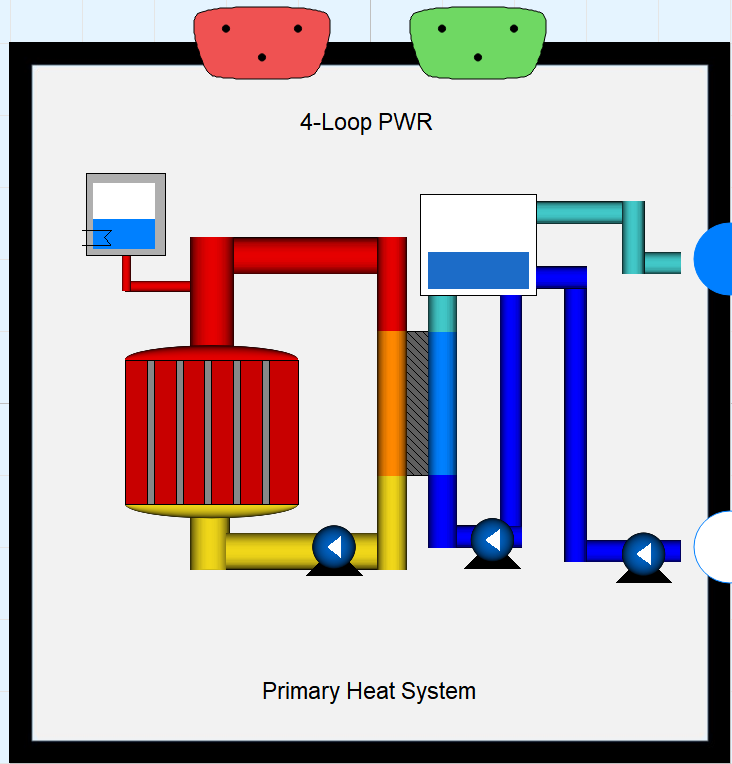
\includegraphics[scale=0.3]{pics/Westinghouse.png}
\caption{Top View of the Four-Loop PWR Plant}
\label{Top View Westinghouse}
\end{figure}


\subsubsection{Generic Modular PWR}
The generic modular PWR unit, Figure \ref{Top View Generic Modular}, is sized to be 160 MWt with 50MWe output as is consistent with the NuScale power module. However, the generic modular PWR does not operate under natural circulation but instead operates under forced flow. Therefore, this unit provides more stability in the code since it does not rely on density differentials to drive flow. This makes the unit less useful than is the NuScale style reactor modeled below, but it does provide the user a power input consistent with NuScale style systems but without the need to tune system geometries, friction factors, etc.. to meet the proper flow dynamics. As with the Westinghouse plant the data file is included in the subsystem  model and has reactivity controls within the core submodule. The Generic Modular PWR relies heavily on the TRANSFORM library for its subcomponents. The steam generator is a once through design with geometrical orientation consistent with a helical coil steam generator. 

\begin{figure}[hbtp]
\centering
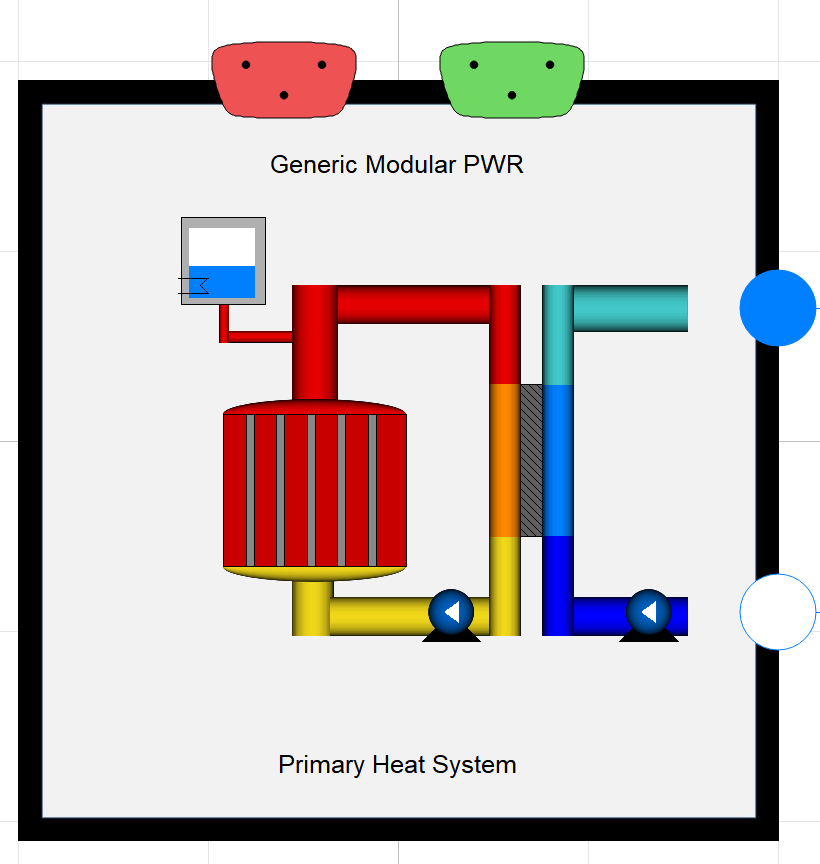
\includegraphics[scale=0.3]{pics/Generic_Modular_PWR.png}
\caption{Top Level Depiction of the Generic Modular PWR in the NHES package.}
\label{Top View Generic Modular}
\end{figure}

% content
\subsubsection{Natural Circulation Small Modular Reactor}
The natural circulation SMR power module,Figure \ref{Top View NuScale Reactor}, is an integral pressurized water reactor (IPWR) that operates with a nominal thermal power of 160 MWt capable of producing 50 MWe to the electric grid. Integral designs are fully self-contained, eliminating the need for large main steam lines that can potentially lead to large break loss of coolant accidents (LOCA). Instead the primary system has only an inlet of feed water into the bottom of the helical coil steam generator and an exit point for steam at the top of the steam generator. All sizes for components is held within the data record in the sub-system. These sizes are consistent with NRC design documentation that can be publicly viewed on the NuScale NRC design certification page. 

The primary system does not include any pumps but instead operates under natural circulation. Natural circulation reactors rely on the height and density differentials between hot and cold water to drive circulation of water through the core. Through elimination of primary coolant pumps an entire class of accident scenarios is eliminated. Modeling efforts in this report focused on three main efforts: matching thermal and electric output, matching system geometry, and matching natural circulation efforts in the system via flow rates and temperature differentials. The primary side of the module has heights and cross-sectional areas in accordance with NRC design certification material. The primary and secondary sides were modeled in their entirety. The helical coil steam generator was modeled as a once through steam generator where the secondary side is on the inside of the tubes and the primary side fluid run along the outside of the tubes.  The full report on this module is available on OSTI \cite{2019NuScaleM4}.


\begin{figure}[hbtp]
\centering
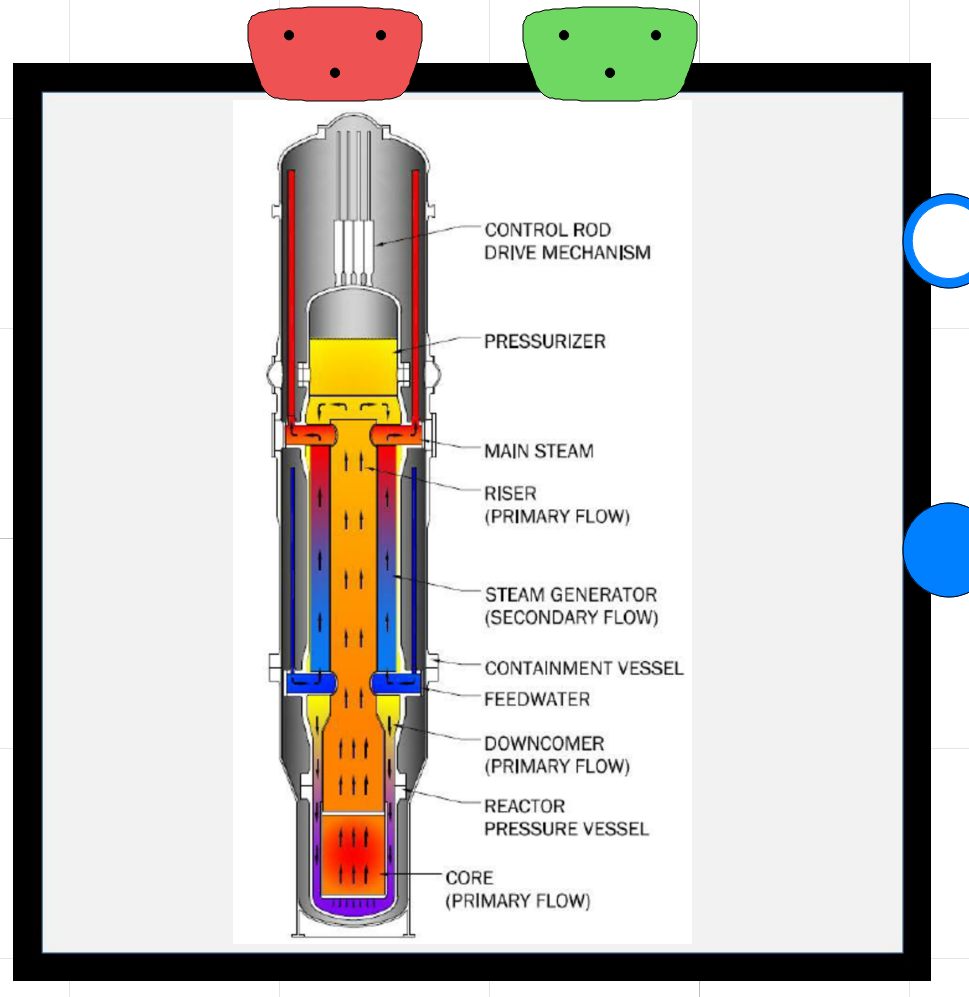
\includegraphics[scale=0.3]{pics/NuScale.png}
\caption{Top Level Depiction of the SMR System in the NHES package.}
\label{Top View NuScale Reactor}
\end{figure}

%\subsection{Cloning the Hybrid Repository}
\label{sec:clone raven}

The first step in installing the package is to clone the HYBRID repository. To do this, use
\begin{lstlisting}[language=bash]
git clone https://github.com/idaholab/HYBRID.git
\end{lstlisting}
This will download the repository into a folder called 'hybrid'. To go inside the folder, use
\begin{lstlisting}[language=bash]
cd hybrid
\end{lstlisting}


\subsubsection{Install RAVEN and its plugins as a sub-module}

The next step is to download and install RAVEN and the submodule (e.g. TEAL, HERON) plugins as a sub-module of the HYBRID repository. 

A submodule allows you to keep another Git repository in a subdirectory of your repository. The other repository has its own history, which does not interfere with the history of the current repository. This can be used to have external dependencies such as third party libraries for example.

In order to get RAVEN do the following in the hybrid folder

\begin{lstlisting}[language=bash]
git checkout devel
\end{lstlisting}

Update the Branch

\begin{lstlisting}[language=bash]
git pull
\end{lstlisting}

to add RAVEN as a submodule
\begin{lstlisting}[language=bash]
git submodule update --init --recursive
\end{lstlisting}

\textbf{Install and Compile RAVEN. }
Once you have downloaded RAVEN as a sub-module, you have to install it. go to the \href{https://github.com/idaholab/raven/wiki/intallationMain}{RAVEN Wiki} for information about how to install it. Run all the tests outlined in the RAVEN wiki. 

\subsubsection{Inform the Framework Paths}

In order to set up the hybrid repository, you must inform the framework about the location of the Dymola python interface. For doing so, navigate to the hybrid directory:

to add RAVEN as a submodule
\begin{lstlisting}[language=bash]
cd <path to your hybrid repository>/hybrid
\end{lstlisting}
Run the following command:
\begin{lstlisting}[language=bash]
./scripts/write_hybridrc.py -p DYMOLA_PATH
\end{lstlisting}

Where DYMOLAPATH is the path to the python interface egg folder in the DYMOLA installation locally. For example:
 
\begin{lstlisting}[language=bash]
./scripts/write_hybridrc.py -p 
	"/c/Program\ Files/Dymola\ 2020x/Modelica/Library/
	python_interface/dymola.egg"
\end{lstlisting}


\subsection{Energy Manifold}
The energy manifolds intention is be a diversion module to as many different subunits as needed for fluid diversion. It consists of a series of pipes that can be extended to “n” submodules, see Figure \ref{Top View Energy Manifold}. The unit has the capability of utilizing control schemes, however in many practical applications the control schemes are encapsulated within the subprocesses as opposed to within the energy manifold. There are currently four potential energy manifolds that can be used. For practical purposes only the model SteamManifold\textunderscore L1\textunderscore boundaries is used in integrated energy systems as it does not include control valves and supports “n” submodules going in and out. The other versions of the energy manifold exist for advanced users in the event the balance of plant or subprocess they are connecting to does not include sufficient valving and control to properly constrain the system. For example, simplified balance of plant systems that do not contain return flow would require the energy manifold to provide makeup water from the condenser, therefore for that scenario we would need to use the SteamManifold\textunderscore L1\textunderscore FWH\textunderscore Cond model which contains a condenser and feedwater heater.   

\begin{figure}[hbtp]
\centering
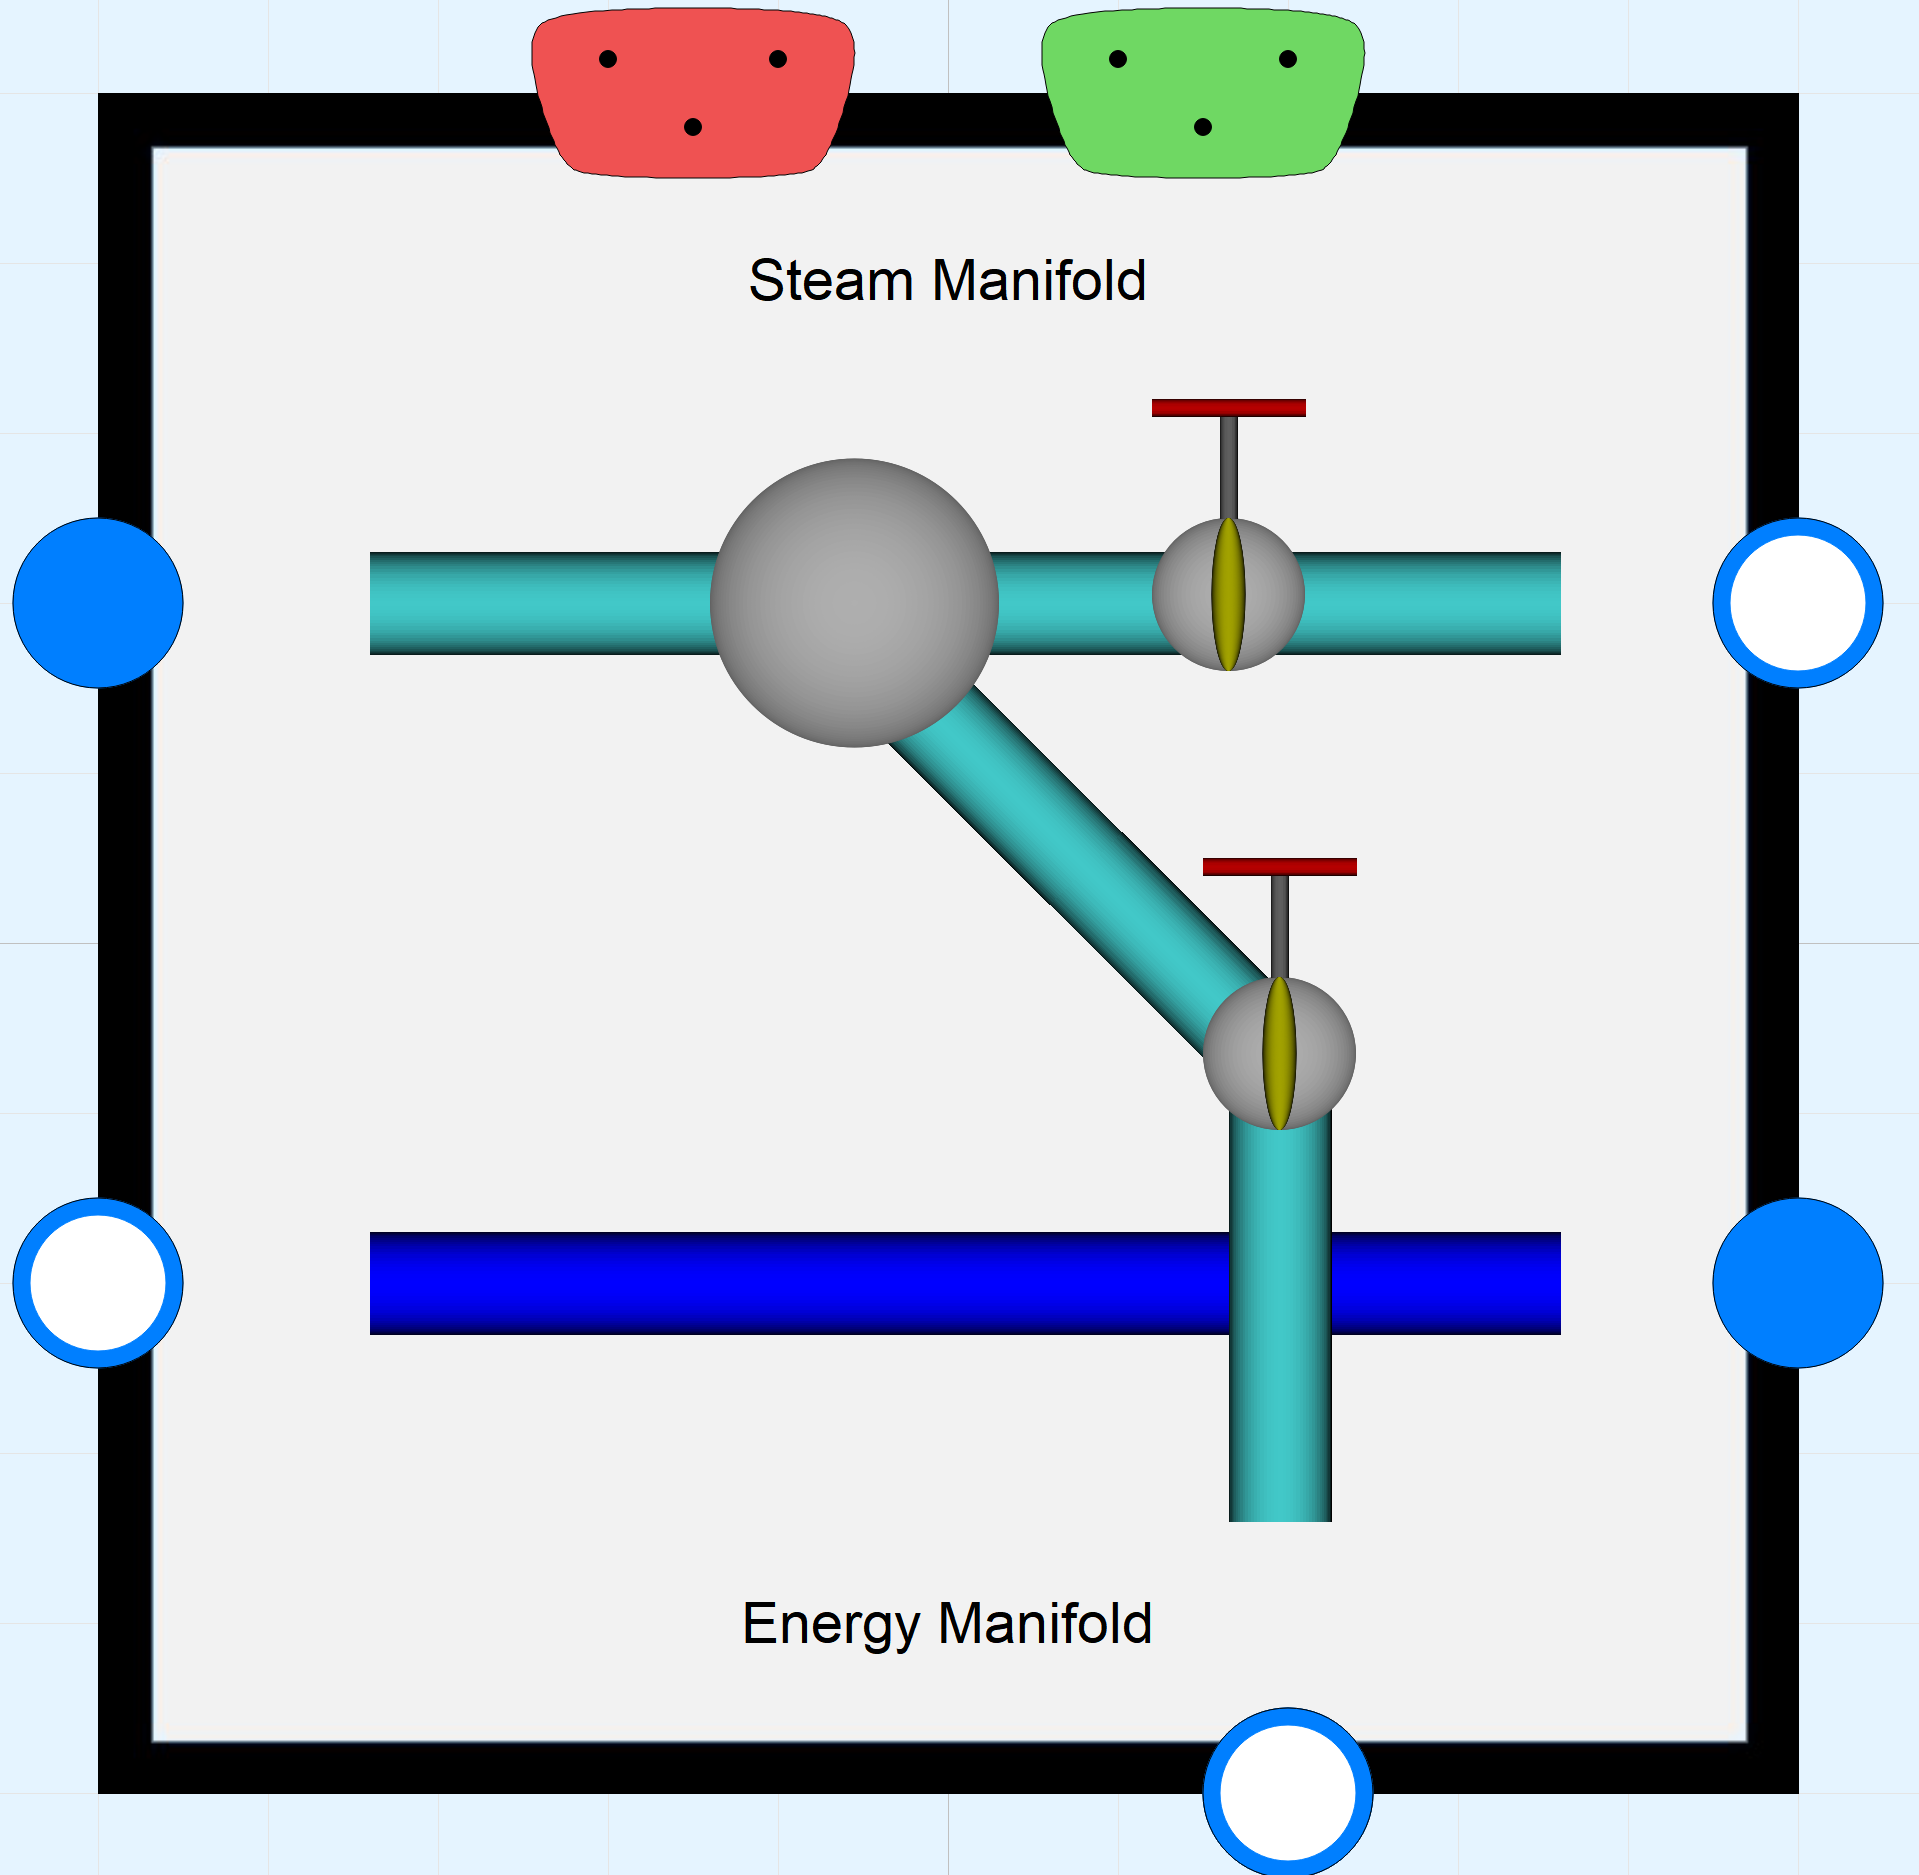
\includegraphics[scale=0.15]{pics/Energy_Manifold.png}
\caption{: Top Level Depiction of the Energy Manifold in the NHES package}
\label{Top View Energy Manifold}
\end{figure}



% content


%\subsection{Cloning the Hybrid Repository}
\label{sec:clone raven}

The first step in installing the package is to clone the HYBRID repository. To do this, use
\begin{lstlisting}[language=bash]
git clone https://github.com/idaholab/HYBRID.git
\end{lstlisting}
This will download the repository into a folder called 'hybrid'. To go inside the folder, use
\begin{lstlisting}[language=bash]
cd hybrid
\end{lstlisting}


\subsubsection{Install RAVEN and its plugins as a sub-module}

The next step is to download and install RAVEN and the submodule (e.g. TEAL, HERON) plugins as a sub-module of the HYBRID repository. 

A submodule allows you to keep another Git repository in a subdirectory of your repository. The other repository has its own history, which does not interfere with the history of the current repository. This can be used to have external dependencies such as third party libraries for example.

In order to get RAVEN do the following in the hybrid folder

\begin{lstlisting}[language=bash]
git checkout devel
\end{lstlisting}

Update the Branch

\begin{lstlisting}[language=bash]
git pull
\end{lstlisting}

to add RAVEN as a submodule
\begin{lstlisting}[language=bash]
git submodule update --init --recursive
\end{lstlisting}

\textbf{Install and Compile RAVEN. }
Once you have downloaded RAVEN as a sub-module, you have to install it. go to the \href{https://github.com/idaholab/raven/wiki/intallationMain}{RAVEN Wiki} for information about how to install it. Run all the tests outlined in the RAVEN wiki. 

\subsubsection{Inform the Framework Paths}

In order to set up the hybrid repository, you must inform the framework about the location of the Dymola python interface. For doing so, navigate to the hybrid directory:

to add RAVEN as a submodule
\begin{lstlisting}[language=bash]
cd <path to your hybrid repository>/hybrid
\end{lstlisting}
Run the following command:
\begin{lstlisting}[language=bash]
./scripts/write_hybridrc.py -p DYMOLA_PATH
\end{lstlisting}

Where DYMOLAPATH is the path to the python interface egg folder in the DYMOLA installation locally. For example:
 
\begin{lstlisting}[language=bash]
./scripts/write_hybridrc.py -p 
	"/c/Program\ Files/Dymola\ 2020x/Modelica/Library/
	python_interface/dymola.egg"
\end{lstlisting}


\subsection{Industrial Process}
Integrated Energy Systems often include thermal and electrical energy users aside the electric grid. To accommodate thermal energy users and byproduct production the HYBRID repository includes a hydrogen production unit and a reverse osmosis unit. 

\subsubsection{Hydrogen Production}
The hybrid repository includes hydrogen production via high temperature steam electrolysis (HTSE) as shown in Figure \ref{Top View HTSE}. HTSE utilizes a combination of thermal energy and electricity to split water into hydrogen (H2) and oxygen (O2) in Solid Oxide Electrolyzer Cells (SOECs), which can be seen in simple terms as the reverse operation of solid oxide fuel cells (SOFCs). The cathode-supported cell consists of a three-layer solid structure (composed of porous cathode, electrolyte, and porous anode) and an interconnect (separator) plate \cite{Udagawa}. An oxygen-ion conducting electrolyte (e.g., yttria-stabilized zirconia [YSZ] or scandia-stabilized zirconia [ScSZ]) is generally used in SOECs \cite{JimObrien}. For electrically conducting electrodes, a nickel cermet cathode, and a perovskite anode such as strontium-doped lanthanum manganite (LSM) are typically used. The interconnect plate separates the process gas streams; it must also be electrically conducting and is usually metallic, such as a ferritic stainless steel. 

For the HTSE models there are four main models developed by INL, each relying on the same underlying physics of the system but with different control schemes. The HTSE units within the Modelica framework have been specifically designed for integration with light water reactor systems and have been sized with the necessary components to allow for steam side preheating under this assumption. It should be noted that in other HTSE designs there may be varying degrees of preheating equipment based on inlet conditions from the external process. For the HTSE process system parameters are finely tuned and highly non-linear when compared with other process models. Changes in heat exchanger design and sizing can be made directly within the subsystem model however due to the nonlinearity of the system convergence following any changes, a singular component cannot be guaranteed. To modify HTSE stack characteristics the user will need to go two levels down into the HTSE stack system the HTSE stack can be clicked on to open a parameter table where stack characteristics can be modified. Due to the high level of complexity required with HTSE stacks and the customization required depending on the inlet conditions of external system usage of the existing HTSE is preferred, with more details available in two reports published. \cite{2016HTSE},\cite{2017HTSE},\cite{JongHydrogen}. Base classes for the HTSE system can found in the “Electrolysis” package within the NHES framework and can be utilized if one desires to create their own HTSE unit. 

\begin{figure}[hbtp]
\centering
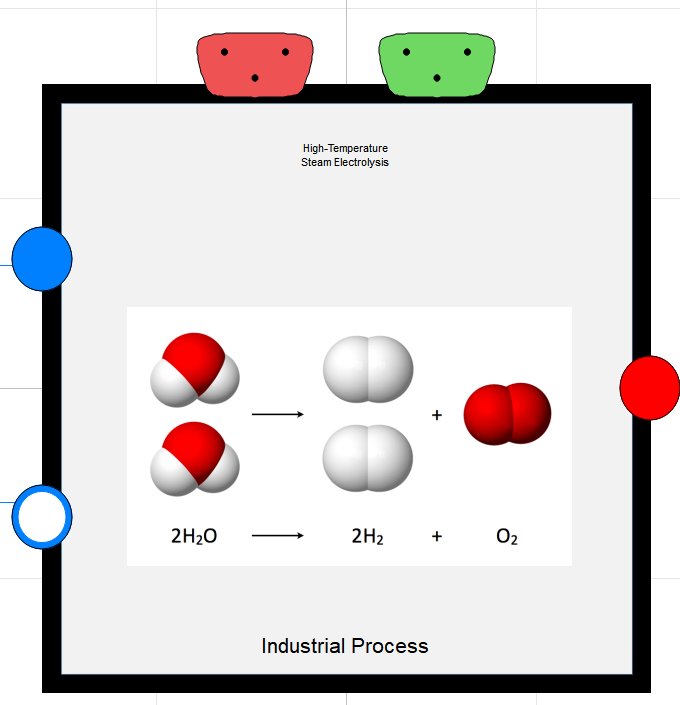
\includegraphics[scale=0.4]{pics/HTSE.png}
\caption{Top Level Depiction of the High Temperature Steam Electrolysis Unit in the NHES package}
\label{Top View HTSE}
\end{figure}



\subsubsection{Desalination}
The NHES repository includes a desalination industrial process based on reverse osmosis (RO), Figure \ref{Top View Reverse Osmosis}, designed for brackish water desalination. RO desalination utilizes a semi-permeable membrane, which allows water to pass through but not salts, thus separating the fresh water from the saline feed water. A typical Brackish Water RO (BWRO) plant consists of four main components: feed water pretreatment, High-Pressure (HP) pumping, membrane separation, and permeate (fresh water) post-treatment. The concentrate water rejected by the first membrane module plays a role as the feed water for the second membrane module by the successive order, and so on. These pressure vessels are arranged in rows in each membrane stage, with two-stage membrane separation being typical in BWRO. Each stage has a recovery of 50–60 percent, achieving overall system recovery of 70–85 percent \cite{JongDesalination}. 

The Reverse Osmosis Subsystem unit provides the user the ability to modify the number of parallel reverse osmosis units being utilized within the plant alongside to specify how much power is being input into the RO system. Each one of these parallel systems is assumed to go through a two-step the desalination process. In addition, the unit provides the user the ability to alter the salinity of the brine coming into the plant alongside a specified pressure differential across the plant. If further alterations and control are desired from a user perspective reports detailing the full specifications of the plant designs are available in \cite{2018ThermalStorage}, \cite{JongDesalination}. Additionally, base components for the entire desalination plant can be found in the “Desalination” package within the NHES repository. 
 

\begin{figure}[hbtp]
\centering
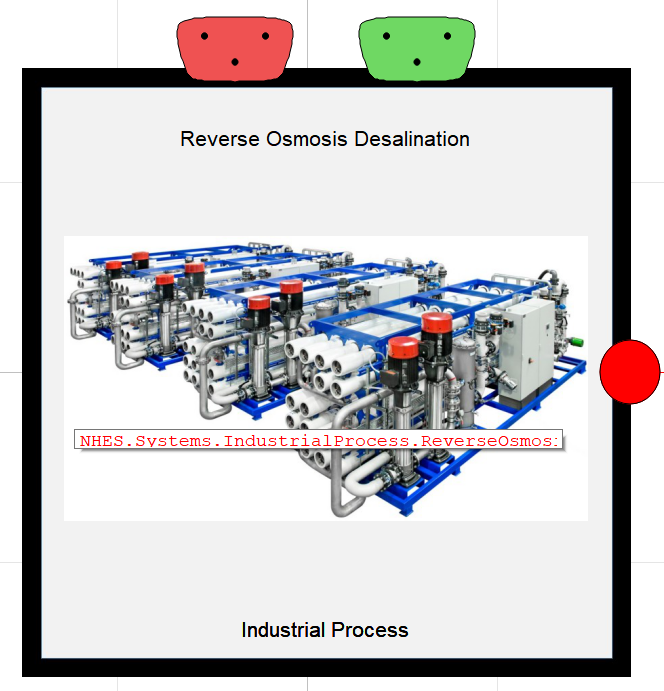
\includegraphics[scale=0.3]{pics/Desalination Plant.png}
\caption{Top Level Depiction of the Brackish Water Desalination Process in the NHES package}
\label{Top View Reverse Osmosis}
\end{figure}



% content


%\subsection{Cloning the Hybrid Repository}
\label{sec:clone raven}

The first step in installing the package is to clone the HYBRID repository. To do this, use
\begin{lstlisting}[language=bash]
git clone https://github.com/idaholab/HYBRID.git
\end{lstlisting}
This will download the repository into a folder called 'hybrid'. To go inside the folder, use
\begin{lstlisting}[language=bash]
cd hybrid
\end{lstlisting}


\subsubsection{Install RAVEN and its plugins as a sub-module}

The next step is to download and install RAVEN and the submodule (e.g. TEAL, HERON) plugins as a sub-module of the HYBRID repository. 

A submodule allows you to keep another Git repository in a subdirectory of your repository. The other repository has its own history, which does not interfere with the history of the current repository. This can be used to have external dependencies such as third party libraries for example.

In order to get RAVEN do the following in the hybrid folder

\begin{lstlisting}[language=bash]
git checkout devel
\end{lstlisting}

Update the Branch

\begin{lstlisting}[language=bash]
git pull
\end{lstlisting}

to add RAVEN as a submodule
\begin{lstlisting}[language=bash]
git submodule update --init --recursive
\end{lstlisting}

\textbf{Install and Compile RAVEN. }
Once you have downloaded RAVEN as a sub-module, you have to install it. go to the \href{https://github.com/idaholab/raven/wiki/intallationMain}{RAVEN Wiki} for information about how to install it. Run all the tests outlined in the RAVEN wiki. 

\subsubsection{Inform the Framework Paths}

In order to set up the hybrid repository, you must inform the framework about the location of the Dymola python interface. For doing so, navigate to the hybrid directory:

to add RAVEN as a submodule
\begin{lstlisting}[language=bash]
cd <path to your hybrid repository>/hybrid
\end{lstlisting}
Run the following command:
\begin{lstlisting}[language=bash]
./scripts/write_hybridrc.py -p DYMOLA_PATH
\end{lstlisting}

Where DYMOLAPATH is the path to the python interface egg folder in the DYMOLA installation locally. For example:
 
\begin{lstlisting}[language=bash]
./scripts/write_hybridrc.py -p 
	"/c/Program\ Files/Dymola\ 2020x/Modelica/Library/
	python_interface/dymola.egg"
\end{lstlisting}


\subsection{Balance of Plant}
There are two main balance of plant models in the hybrid repository. The standard ideal turbine (with and without a condenser and feedwater heater) and step down turbines that allow turbine tap offtake.


\subsubsection{Simple Balance of Plant}

The balance of plant system consists of an ideal steam turbine model, a condenser, feedwater system for reheat, and a couple of valves that allow steam flow either to the turbine or as bypass to the condenser, Figure \ref{Top View SimpleBOP}. Additionally, piping exists to send condensate and rejected heat from ancillary processes directly to the condenser. The balance of plant model can handle supervisory control input for direct control of the turbine control valve and turbine bypass valve based on different sensor input. The main balance of plant system is designed to model Rankine systems.  

\begin{figure}[hbtp]
\centering
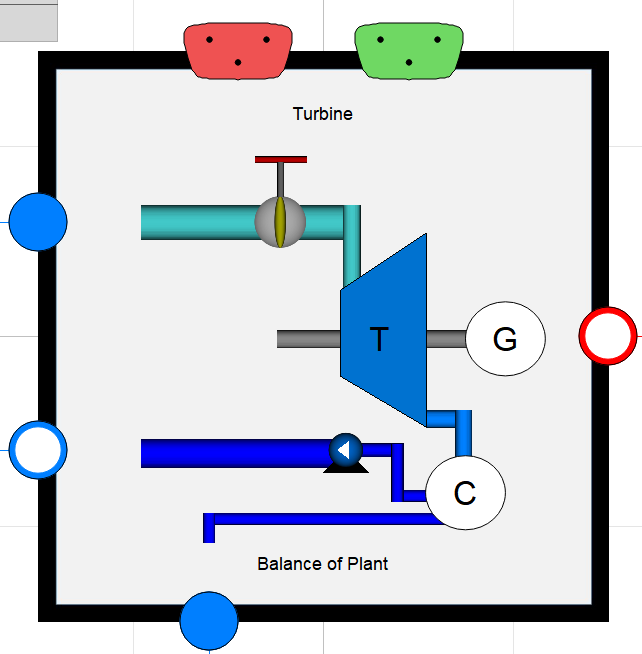
\includegraphics[scale=0.4]{pics/BOP.png}
\caption{Top Level Depiction of the Balance of Plant in the NHES package}
\label{Top View SimpleBOP}
\end{figure}


\subsubsection{Step Down Turbines}

The step-down turbines consist of a series of an ideal steam turbines connected via a singular rotational inertia shaft with bypass tap lines coming off the turbines, Figure \ref{Top View Step Down Turbines}. The purpose of this model is to allow turbine tap offtake in a dynamic system. The data record within the model includes a series of inputs that allows the user to specify the turbine tap offtake pressures. Additionally, each individual offtake fraction can be input from the data record. The outlet of the stepdown turbines does not include a condenser; therefore, a condenser model would need to be included in a separate system model if the fluid is to be re-introduced into an overall system model.
 
\begin{figure}[hbtp]
\centering
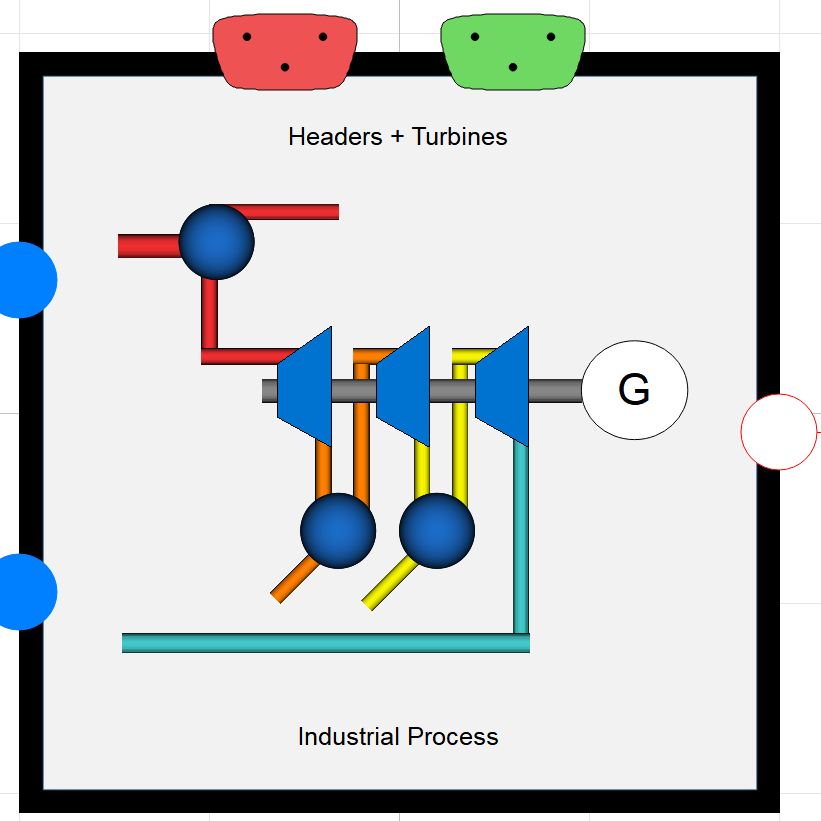
\includegraphics[scale=0.3]{pics/HeaderStepdownturbines.png}
\caption{Top Level Depiction of the StepDown Turbines in the NHES package}
\label{Top View Step Down Turbines}
\end{figure}


\subsubsection{Stage by Stage Turbine}
The stage by stage turbine package is designed to allow for detailed design of a Rankine cycle: including all turbine taps, moisture separators, reheaters, fluid junctions, and peaking capabilities. The model uses geometric design rather than system design (pressure ratios, setpoints, efficiencies). The primary design values are cross sectional and design flow deflection angles. Pressure, mass flow rate, and entropic efficiency are all uncontrolled and unspecified. 


\begin{figure}[hbtp]
\centering
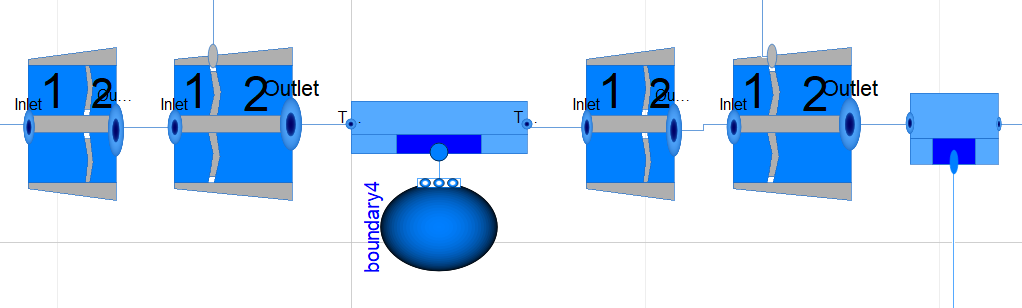
\includegraphics[scale=0.75]{pics/StagebyStageTurbine.png}
\caption{Top Level Stage by Stage Turbine Section With Stators, Rotors, a Tap, and a Moisture Separator}
\label{TVSbST}
\end{figure}


There are 8 primary components used to develop a full stage by stage turbine system. Multiple are shown in Figure \ref{TVSbST}. The first are the turbine inlet and turbine outlet components which allow for transition between 1D axial fluid components and 3D velocity cylindrical fluid flow components. The next components are the stator and rotor stages. Stator stages deflect incoming flow to better impinge and deposit energy on rotating rotor stages. Rotor stages additionally have torque connectors to connect to a physical turbine model which is responsible for linking the rotor stage torque to the electrical generator. T-junction components setup for cylindrical flow connectors allow for overpowering a rated turbine flow. The final two components deal with removing flow from the turbine. One is a turbine tap, which sets pressures equal between stages. The other is a moisture separator that removes a specific fraction of liquid flow quality. 

The stage by stage turbine has been tested from 50-100 percent steam flow. 


% content


%\subsection{Cloning the Hybrid Repository}
\label{sec:clone raven}

The first step in installing the package is to clone the HYBRID repository. To do this, use
\begin{lstlisting}[language=bash]
git clone https://github.com/idaholab/HYBRID.git
\end{lstlisting}
This will download the repository into a folder called 'hybrid'. To go inside the folder, use
\begin{lstlisting}[language=bash]
cd hybrid
\end{lstlisting}


\subsubsection{Install RAVEN and its plugins as a sub-module}

The next step is to download and install RAVEN and the submodule (e.g. TEAL, HERON) plugins as a sub-module of the HYBRID repository. 

A submodule allows you to keep another Git repository in a subdirectory of your repository. The other repository has its own history, which does not interfere with the history of the current repository. This can be used to have external dependencies such as third party libraries for example.

In order to get RAVEN do the following in the hybrid folder

\begin{lstlisting}[language=bash]
git checkout devel
\end{lstlisting}

Update the Branch

\begin{lstlisting}[language=bash]
git pull
\end{lstlisting}

to add RAVEN as a submodule
\begin{lstlisting}[language=bash]
git submodule update --init --recursive
\end{lstlisting}

\textbf{Install and Compile RAVEN. }
Once you have downloaded RAVEN as a sub-module, you have to install it. go to the \href{https://github.com/idaholab/raven/wiki/intallationMain}{RAVEN Wiki} for information about how to install it. Run all the tests outlined in the RAVEN wiki. 

\subsubsection{Inform the Framework Paths}

In order to set up the hybrid repository, you must inform the framework about the location of the Dymola python interface. For doing so, navigate to the hybrid directory:

to add RAVEN as a submodule
\begin{lstlisting}[language=bash]
cd <path to your hybrid repository>/hybrid
\end{lstlisting}
Run the following command:
\begin{lstlisting}[language=bash]
./scripts/write_hybridrc.py -p DYMOLA_PATH
\end{lstlisting}

Where DYMOLAPATH is the path to the python interface egg folder in the DYMOLA installation locally. For example:
 
\begin{lstlisting}[language=bash]
./scripts/write_hybridrc.py -p 
	"/c/Program\ Files/Dymola\ 2020x/Modelica/Library/
	python_interface/dymola.egg"
\end{lstlisting}


\subsection{Energy Storage}
Energy Storage is a large component of Integrated Energy Systems. Currently there are two models of Energy Storage in the repository. Electric Battery Storage, characterized largely as Li-ion battery technology, and two-tank sensible heat thermal energy storage that uses Therminol-66 as the working fluid. 


\subsubsection{Electric Battery Storage}

Electric Battery Storage, shown in Figure \ref{Top View Logical Battery}, is largely characterized as fast and expensive. Due to the speed with which battery storage systems operate, on the order milliseconds, the battery within the hybrid repository has been modeled as a simple logical battery system. The battery can both charge and discharge based upon the direction of electricity flow through the port. It is assumed to be a “perfect” battery and due to the speed of the system, subcomponents have not been modeled simply because they would operate faster than would be useful for the types of analysis utilized with the system. The battery has user-based inputs that control how fast or slow the system can charge and discharge as well as how much energy can be stored within the battery before it is considered full.   

\begin{figure}[hbtp]
\centering
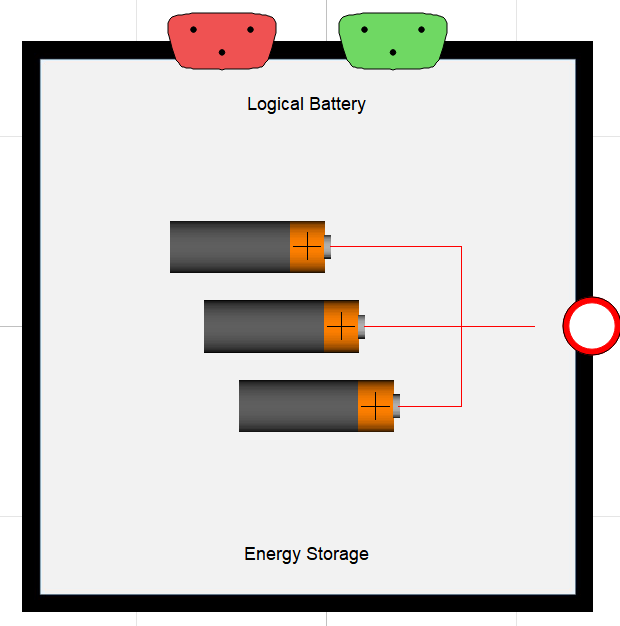
\includegraphics[scale=0.4]{pics/Battery_Storage.png}
\caption{Top Level Depiction of the Logical Battery in the NHES package}
\label{Top View Logical Battery}
\end{figure}


\subsubsection{Two-Tank Thermal Energy Storage}

Sensible heat storage involves the heating of a solid or liquid without phase change and can be deconstructed into two operating modes: charging and discharging. A two-tank TES system, shown in Figure \ref{Top View Two Tank Sensible Storage}, is a common configuration for liquid sensible heat systems. In the charging mode cold fluid is pumped from a cold tank through an Intermediate Heat Exchanger (IHX), heated, and stored in a hot tank while the opposite occurs in the discharge mode. Such systems have been successfully demonstrated in the solar energy field as a load management strategy. The configuration of the TES system held within the repository involves an outer loop interfaces with the energy manifold. Bypass steam is directed through an IHX and ultimately discharged to the main condenser of an Integrated system. An inner loop containing a TES fluid consists of two large storage tanks along with several pumps to transport the TES fluid between the tanks, the IHX and a steam generator. Flow Bypass Valves (FBVs) are included in the discharge lines of both the “hot” and “cold” tanks to prevent deadheading the pumps when the Flow Control Valves (FCVs) are closed. Therminol-66 is chosen as the TES fluid as it is readily available, can be pumped at low temperatures, and offers thermal stability over the range (-3°C–343°C) which covers the anticipated operating range of the light water reactor systems (203°C–260°C). Molten salts (e.g. 48 percent  NaNO3 – 52 percent KNO3) were not considered, as the anticipated operating temperatures fall below their 222°C freezing temperature. The TES system is designed to allow the power plant to run continuously at ~100 percent power over a wide range of operating conditions. During periods of excess capacity, bypass steam is directed to the TES unit through the auxiliary bypass valves where it condenses on the shell side of the IHX. TES fluid is pumped from the cold tank to the hot tank through the tube side of the IHX at a rate sufficient to raise the temperature of the TES fluid to some set point. The TES fluid is then stored in the hot tank at constant temperature. Condensate is collected in a hot well below the IHX and drains back to the main condenser or can be used for some other low pressure application such as chilled water production, desalination or feed-water heating. The system is discharged during periods of peak demand, or when process steam is desired, by pumping the TES fluid from the hot tank through a boiler (steam generator) to the cold tank. This process steam can then be reintroduced into the power conversion cycle for electricity production or directed to some other application through the PCV. A nitrogen cover gas dictates the tank pressures during charging and discharging operation. Full details of the model and its use within integrated energy systems can be found in report \cite{2018ThermalStorage}, \cite{FrickThermalStorage}. 

The model itself is coded in a non-conventional manner compared to the rest of the modelica models. It is coded in an input, output sense rather than in a fluid-port, electric-port based modeling system. This is because the model was transferred over from a FORTRAN style code rather than initially coded in Modelica. To modify the two-tank thermal storage system the user will need to look at each individual model within the charging mode and the discharge mode. Base components within the models are fully commented within the code. Like the HTSE the thermal storage unit is finely tuned and thus use outside of its current state will take a bit of work. To help with this the thermal storage unit has been sized to be compatible for varying sizes of offtake from a power unit. One is sized to take 20 percent of nominal steam from a standard 3400MWt Westinghouse plant, and one is designed for 5 percent offtake. Both designed to provide energy back as a peaking unit. The peaking unit is held within the discharge side of the model and is assumed to have its own turbine or is sent back to the low-pressure turbine. Explicit modeling of the coupling back with the low-pressure turbine has not been done. Future updating of the two-tank thermal storage unit to be consistent with other models is planned.

 
\begin{figure}[hbtp]
\centering
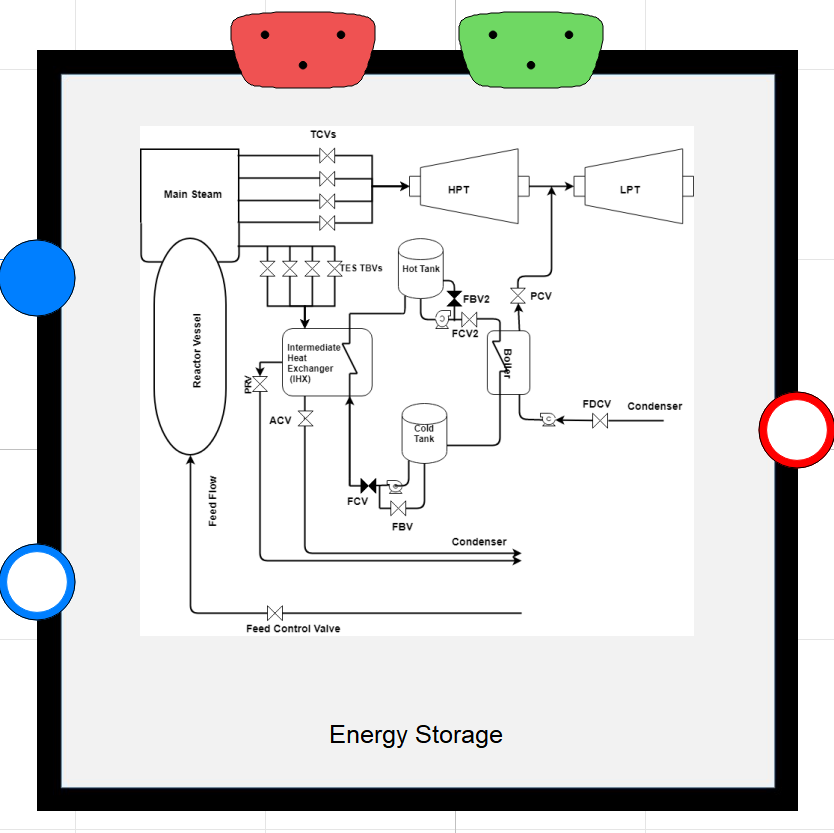
\includegraphics[scale=0.3]{pics/Sensible_Heat_System.png}
\caption{Top Level Depiction of the Two-Tank Sensible Heat Storage Unit in the NHES package}
\label{Top View Two Tank Sensible Storage}
\end{figure}

% content
\subsubsection{Thermocline Packed Bed Thermal Energy Storage}
A thermocline storage system, shown in Figure \ref{Top View Thermocline}, stores heat via hot and cold fluid separated by a thin thermocline region that arises due to density differential between the fluid. Assuming low mixing via internal flow characteristics and structural design, this thermocline region can be kept relatively small in comparison with the size of the tank. Additionally, large buoyancy changes and low internal thermal conductivity are also extremely useful in maintaining small relative thermocline thickness.

To increase the cost-effective nature of these designs, it is common to fill the tank with a low-cost filler material, such as concrete or quartzite. These filler materials are cheap, have high density, and high thermal conductivity. By using such material, a reduction in the amount of high cost thermal fluid can be achieved, thereby increasing the economic competitiveness of such designs.

The thermocline system was modeled from a modified set of Schumann equations that were originally introduced in 1927 \cite{Schumann}. The equation set governs energy conservation of fluid flow through porous media. His equation set has been widely adopted in the analysis of thermocline storage tanks. The modified equations adopted a new version of the convective heat-transfer coefficient to incorporate low and no-flow conditions from Gunn in 1978 \cite{specialHeattransfer}. Additionally, a conductive heat-transfer term was added for the heat conduction through the walls of the tank. Self-degradation of the thermocline in the axial direction is neglected due to low relative values when during standard operation, this is a known limit of the model during times of no flow.

\begin{figure}[hbtp]
\centering
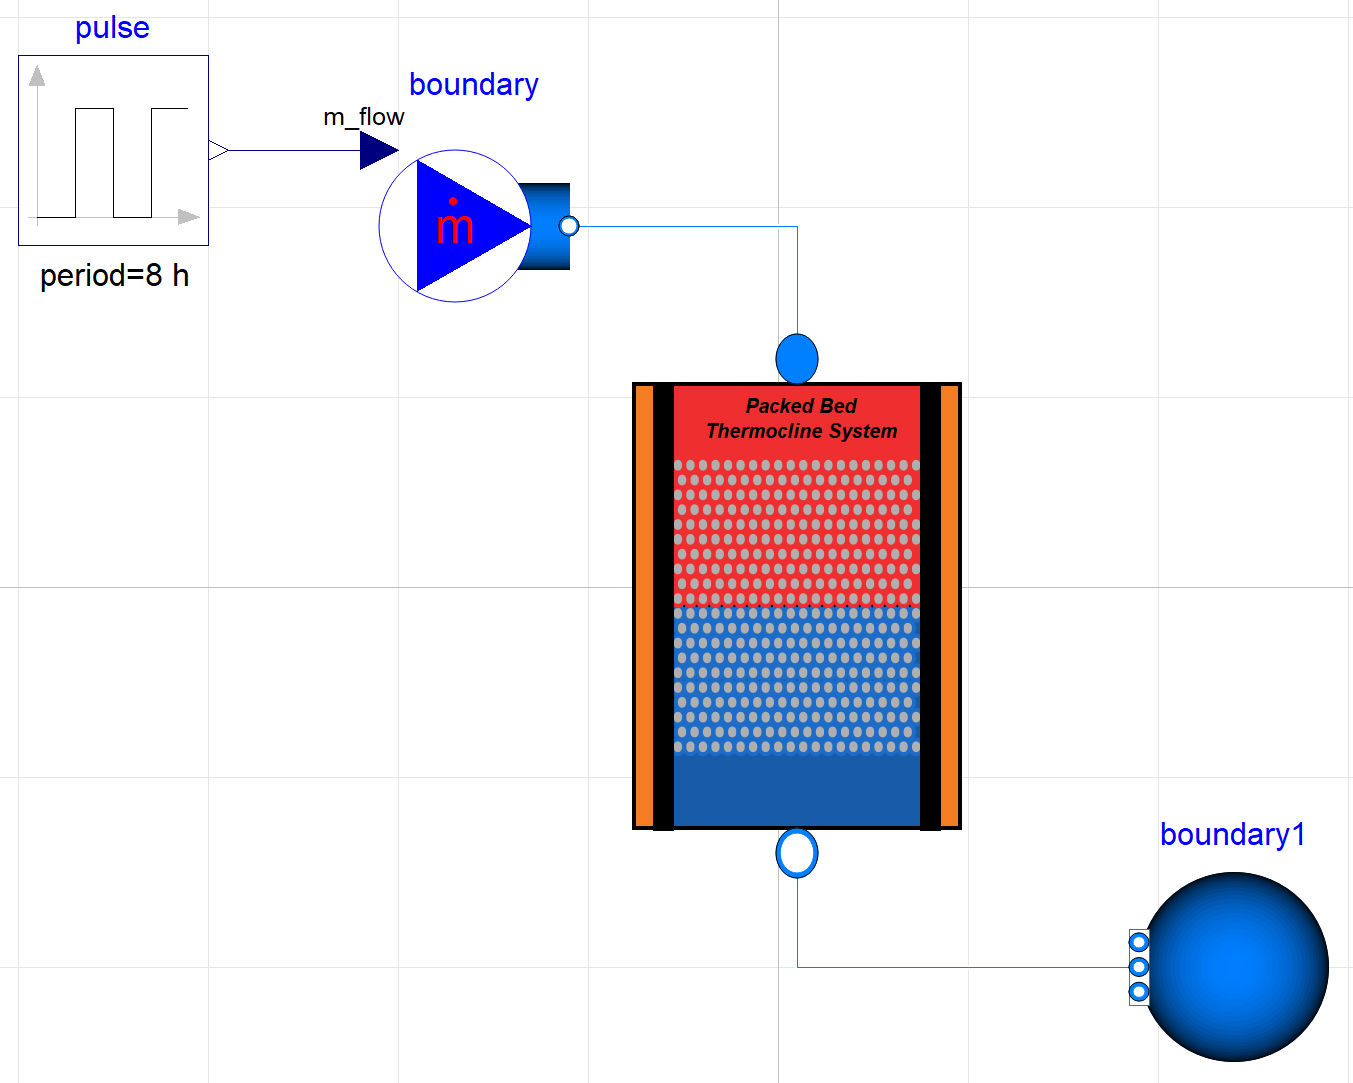
\includegraphics[scale=0.3]{pics/Thermocline_Test.png}
\caption{Top Level Depiction of the Single Tank Packed Bed Heat Storage Unit in the NHES package}
\label{Top View Thermocline}
\end{figure}

\subsubsection{Concrete Solid Media Storage}

Three different models exist for concrete solid media storage, shown in Figure \ref{CTES}. Concrete solid media storage uses inexpensive materials to charge and discharge heat from a fluid system. The models within the Hybrid system use HeatCrete as the concrete material, the properties of which are found in literature. The initial development has been done with energy arbitrage for a Rankine system in mind. However, there are not limitations on the heat transfer fluid that can be used in conjunction with the concrete system. Two design modalities exist with the three developed models. One is a single pipe model and the other is a dual pipe model. All models use simplified flow models: a single pressure and mass flow rate is imposed within a pipe (which allows for significantly improved performance at low and no flow rate conditions) leaving the dynamics of the system to primarily be described by the conservation of energy equation. Within the concrete model, heat conducts both radially and axially in a 2-D nodalized vector. All models calculate values for an average pipe and the system behavior is then scaled by the number of pipes. 

The single pipe model is so called because it only models one fluid pipe within a concrete system. This modeling choice imposes a restriction that heat transfer fluid only flows in one direction or the other (note, no error signals are sent by this, m\textunderscore flow\textunderscore internal = m\textunderscore flow\textunderscore ch-m\textunderscore flow\textunderscore dis). The behavior of this system lends itself better to batch energy applications. The power level during quenching (HTF quenching during charging or concrete quenching during discharging) is an order of magnitude higher than the steady power level. The pressure of the system is taken at the cold end, and defaults to the charging pressure. This model can operate in charging, discharging, OR standby mode. The single pipe model operates with an established axial thermocline and a reversing radial thermal gradient depending on operation. 

The dual pipe and dual pipe two HTFs model contain separate pipes for the charging and discharging flow. This model operates more steadily over long periods of time. Heat is always conducted within the CTES and between the concrete and the HTFs. The dual pipe CTES can operate in charging, discharging, standby, or thermal buffer (both charging and discharging) modes. The dual pipe system operates with mono-directional thermal gradients in both axial and radial directions in all operating modes. 


\begin{figure}[hbtp]
\centering
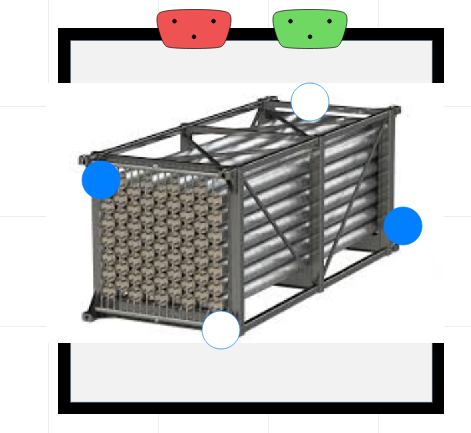
\includegraphics[scale=0.8]{pics/CTES.png}
\caption{Top Level Depiction of Concrete Thermal Energy Storage System}
\label{CTES}
\end{figure}

%\subsection{Cloning the Hybrid Repository}
\label{sec:clone raven}

The first step in installing the package is to clone the HYBRID repository. To do this, use
\begin{lstlisting}[language=bash]
git clone https://github.com/idaholab/HYBRID.git
\end{lstlisting}
This will download the repository into a folder called 'hybrid'. To go inside the folder, use
\begin{lstlisting}[language=bash]
cd hybrid
\end{lstlisting}


\subsubsection{Install RAVEN and its plugins as a sub-module}

The next step is to download and install RAVEN and the submodule (e.g. TEAL, HERON) plugins as a sub-module of the HYBRID repository. 

A submodule allows you to keep another Git repository in a subdirectory of your repository. The other repository has its own history, which does not interfere with the history of the current repository. This can be used to have external dependencies such as third party libraries for example.

In order to get RAVEN do the following in the hybrid folder

\begin{lstlisting}[language=bash]
git checkout devel
\end{lstlisting}

Update the Branch

\begin{lstlisting}[language=bash]
git pull
\end{lstlisting}

to add RAVEN as a submodule
\begin{lstlisting}[language=bash]
git submodule update --init --recursive
\end{lstlisting}

\textbf{Install and Compile RAVEN. }
Once you have downloaded RAVEN as a sub-module, you have to install it. go to the \href{https://github.com/idaholab/raven/wiki/intallationMain}{RAVEN Wiki} for information about how to install it. Run all the tests outlined in the RAVEN wiki. 

\subsubsection{Inform the Framework Paths}

In order to set up the hybrid repository, you must inform the framework about the location of the Dymola python interface. For doing so, navigate to the hybrid directory:

to add RAVEN as a submodule
\begin{lstlisting}[language=bash]
cd <path to your hybrid repository>/hybrid
\end{lstlisting}
Run the following command:
\begin{lstlisting}[language=bash]
./scripts/write_hybridrc.py -p DYMOLA_PATH
\end{lstlisting}

Where DYMOLAPATH is the path to the python interface egg folder in the DYMOLA installation locally. For example:
 
\begin{lstlisting}[language=bash]
./scripts/write_hybridrc.py -p 
	"/c/Program\ Files/Dymola\ 2020x/Modelica/Library/
	python_interface/dymola.egg"
\end{lstlisting}


\subsubsection{Latent Heat Thermal Energy Storage}

Latent heat energy storage stores energy in materials undergoing phase change. These phase change materials (PCMs) can undergo melting and fusion, boiling and condensation, or hydration and dehydration. PCMs have high volumetric and mass-specific energy storage densities. They can theoretically operate isothermally as the phase change occurs at a single temperature. The ideal PCM would have a large latent heat associated with its phase change, little to no density change between phases, indefinite cyclability between phases, and high thermal conductivity. Research continues in PCMs to identify enhancements that would allow lab-scale experiments to increase size to demonstrate grid-scale applications. A significant challenge is enhancing the thermal conductivity in the PCMs. As the charging or discharging HTF will drive the phase change condition at the heat transfer surface, continuing that process into the PCM mass is based on the thermal conductivity of the material. Conductivity enhancement via geometry specification, micro-encapsulation, and material impregnation has been investigated over time. 

The most common PCMs identified operate between the solid and liquid phases where the density change is minimal. Because the melting or solidification front is key to moving heat between the HTF and the PCMs, many high-fidelity models have been developed across the research field. The model available in the HYBRID repository is based on a paraffin wax experiment. The experiment used water as the HTF to melt and solidify paraffin wax. The original model was built in Star-CCM+ and then converted to Matlab. The Matlab version subsequently has been converted into a Modelica model within HYBRID. The generalized low-fidelity model has been built to accommodate new geometric designs, materials, and HTFs. 


The model is a two-dimensional radial conductivity model across three materials: the HTF, a pipe wall, then through the PCM as shown in Figure \ref{PCM}. Within the fluid, the following equation set applies. The equations are also applied within the tube, but the velocity term disappears without internal mass movement. The term $\alpha$ is thermal resistance, equal to thermal conductivity divided by the density and specific heat capacity. 


\[\frac{dT}{dt} = \alpha\nabla^{2}T - (\overrightarrow{v}\cdot\nabla T)\]

Effectively, the equation set is applied across the material interfaces, with an effective interface thermal conductivity

\[k_{eff}=\frac{2k_{1}k_{2}}{k_{1}+k_{2}}\]

Because there is phase change within the PCM. The equation is written in terms of enthalpy instead of temperature, and the PCM temperature is calculated as a function of the enthalpy (h). 

\[\frac{dh}{dt} = \alpha\nabla^{2}h\]

\begin{figure}[hbtp]
\centering
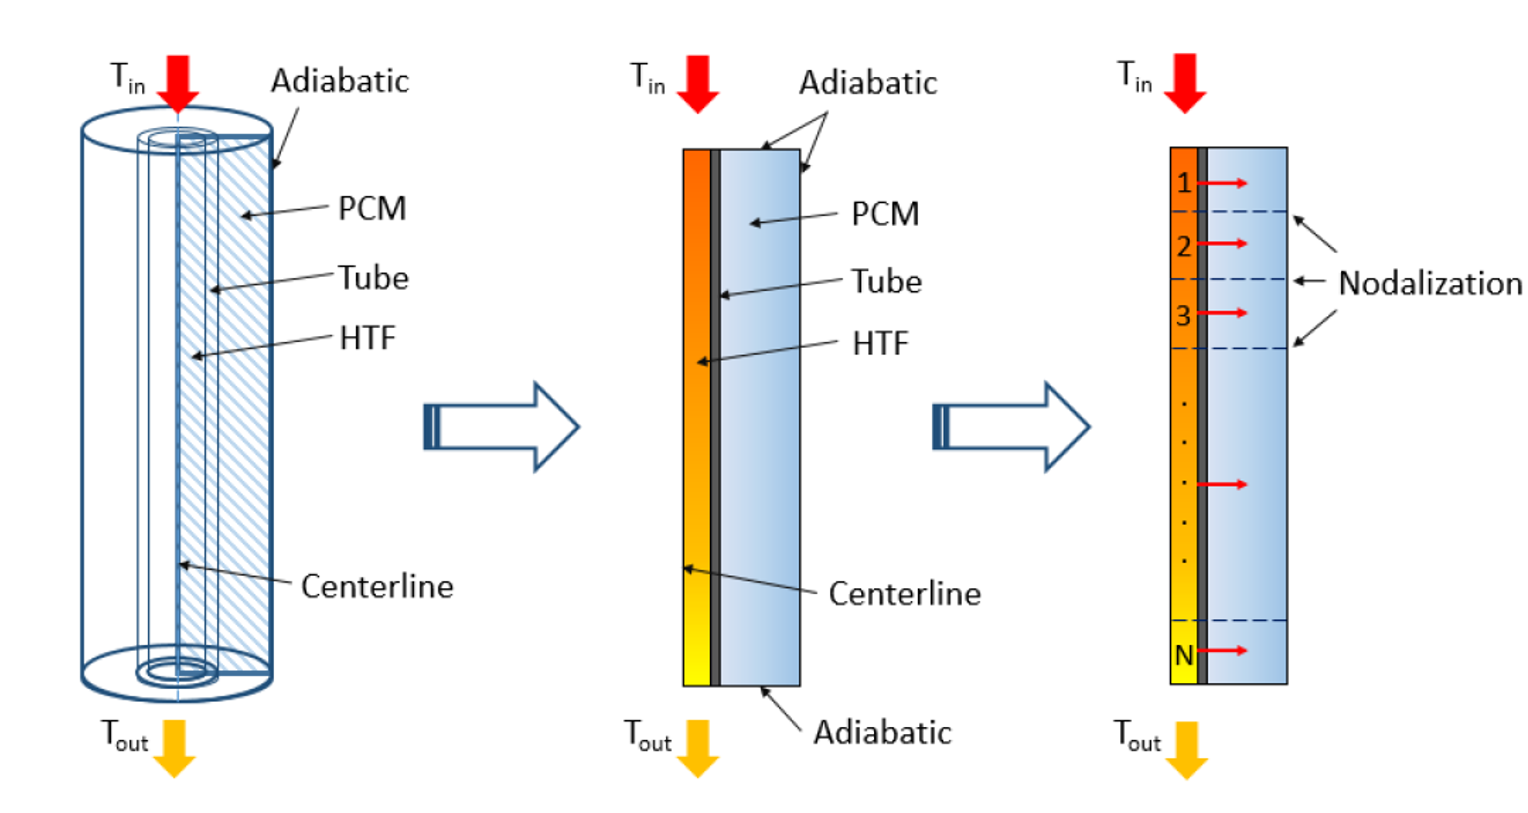
\includegraphics[scale=0.5]{pics/PCM.png}
\caption{PCM Nodalization diagram}
\label{PCM}
\end{figure}

The initial models built in Matlab and Star-CCM+ used constant fluid properties and an assumed inlet velocity. The Modelica model has a fluid inlet and exit to allow for replacement of the HTF in the model, and for outer conditions to dictate to the PCM model the fluid conditions at the interfaces. 





\subsection{Secondary Energy Source}
Secondary Energy Sources, or commonly known as peaking units, are an essential part of the energy grid. These systems provide "on-demand" energy during moments when the electrical demand is larger than what the rest of the grid can accomodate. A common feature of 

\subsubsection{Natural Gas Fired Turbine}

Recently, natural gas-fired turbines have found widespread use because of their higher efficiencies, lower capital costs, shorter installation times, abundance of natural gas supplies, lower greenhouse gas emissions compared to other energy sources; and fast start-up capability, which enables them to be used as peaking units that respond to peak demands \cite{GasTurbine2008}, \cite{GasTurbine2013}. Due to their special characteristics, natural gas fired turbines are installed in numerous places around the world and have become an important source for power generation. This section is dedicated to detailed process and control designs of the GTPP, whose primary role is to cover rapid dynamics in grid demand that cannot be met by the remainder of the N-R HES. Simulation results involving several case studies are also provided. Full system details are available in OSTI \cite{2016HTSE}.

The natural gas turbine, Figure \ref{Top View Gas Turbine}, is designed with parameters embedded in each individual component. The top level variables can be edited directly within the GTTP\textunderscore PowerCtrl system. This component is where things such as pressure ratios, flow rates, mechanical efficiencies, and shaft inertia can be modified. The natural gas turbine is designed with a nominal electrical power generation capacity of 35MWe but has a specially designed capacityScaler variable that allows the user to scale the system to between 17 and 70MWe for a singular load. If more are desired then the deployment of several natural gas fired turbines would be required. 

\begin{figure}[hbtp]
\centering
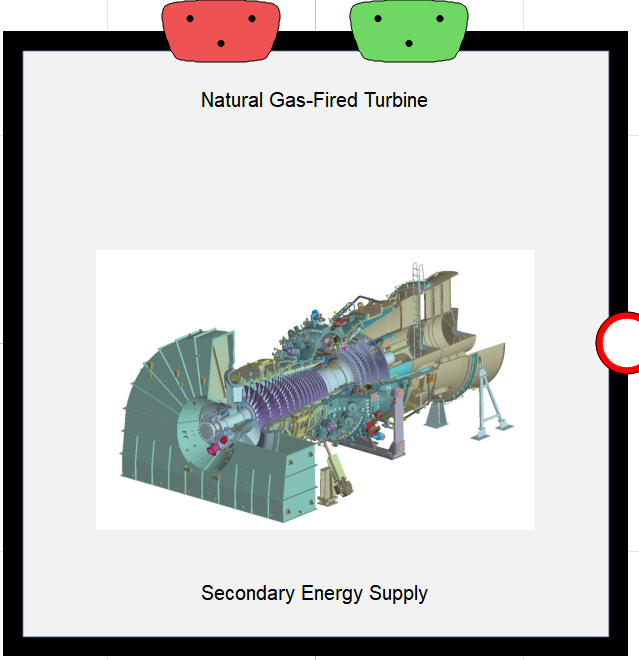
\includegraphics[scale=0.4]{pics/GasTurbine.png}
\caption{Top Level Depiction of the Natural Gas Fired Turbine in the NHES package}
\label{Top View Gas Turbine}
\end{figure}

\subsubsection{Hydrogen Turbine}
With the increase in hydrogen production technologies comes on the other end hydrogen burning technologies. To accommodate a hydrogen burning technology the HYBRID repository has been outfitted with a retrofit natural gas burner that is capable of handling pure hydrogen. 

The hydrogen turbine, Figure \ref{Top View Hydrogen Turbine}, is designed with parameters embedded in each individual component. The top level variables can be edited directly within the Hydrogen\textunderscore PowerCtrl system. This component is where things such as pressure ratios, flow rates, mechanical efficiencies, and shaft inertia can be modified. The hydrogen turbine is designed with a nominal electrical power generation capacity of 35MWe but has a specially designed capacityScaler variable that allows the user to scale the system to between 17 and 70MWe for a singular load. If more are desired then the deployment of several hydrogen turbines would be required. 


\begin{figure}[hbtp]
\centering
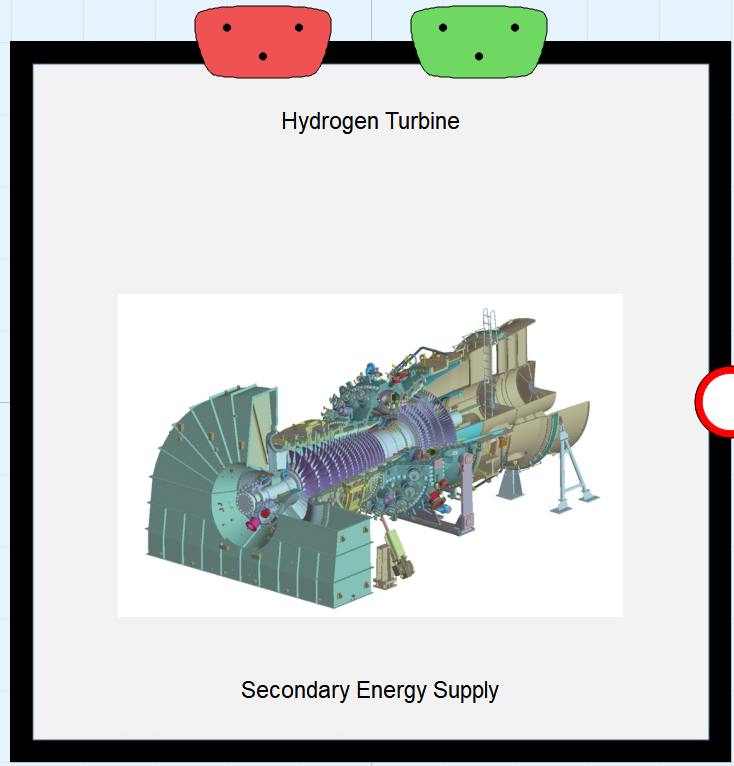
\includegraphics[scale=0.4]{pics/Hydrogen_Turbine.png}
\caption{Top Level Depiction of the Hydrogen Turbine in the NHES package}
\label{Top View Hydrogen Turbine}
\end{figure}
%\subsection{Cloning the Hybrid Repository}
\label{sec:clone raven}

The first step in installing the package is to clone the HYBRID repository. To do this, use
\begin{lstlisting}[language=bash]
git clone https://github.com/idaholab/HYBRID.git
\end{lstlisting}
This will download the repository into a folder called 'hybrid'. To go inside the folder, use
\begin{lstlisting}[language=bash]
cd hybrid
\end{lstlisting}


\subsubsection{Install RAVEN and its plugins as a sub-module}

The next step is to download and install RAVEN and the submodule (e.g. TEAL, HERON) plugins as a sub-module of the HYBRID repository. 

A submodule allows you to keep another Git repository in a subdirectory of your repository. The other repository has its own history, which does not interfere with the history of the current repository. This can be used to have external dependencies such as third party libraries for example.

In order to get RAVEN do the following in the hybrid folder

\begin{lstlisting}[language=bash]
git checkout devel
\end{lstlisting}

Update the Branch

\begin{lstlisting}[language=bash]
git pull
\end{lstlisting}

to add RAVEN as a submodule
\begin{lstlisting}[language=bash]
git submodule update --init --recursive
\end{lstlisting}

\textbf{Install and Compile RAVEN. }
Once you have downloaded RAVEN as a sub-module, you have to install it. go to the \href{https://github.com/idaholab/raven/wiki/intallationMain}{RAVEN Wiki} for information about how to install it. Run all the tests outlined in the RAVEN wiki. 

\subsubsection{Inform the Framework Paths}

In order to set up the hybrid repository, you must inform the framework about the location of the Dymola python interface. For doing so, navigate to the hybrid directory:

to add RAVEN as a submodule
\begin{lstlisting}[language=bash]
cd <path to your hybrid repository>/hybrid
\end{lstlisting}
Run the following command:
\begin{lstlisting}[language=bash]
./scripts/write_hybridrc.py -p DYMOLA_PATH
\end{lstlisting}

Where DYMOLAPATH is the path to the python interface egg folder in the DYMOLA installation locally. For example:
 
\begin{lstlisting}[language=bash]
./scripts/write_hybridrc.py -p 
	"/c/Program\ Files/Dymola\ 2020x/Modelica/Library/
	python_interface/dymola.egg"
\end{lstlisting}




%\subsection{Conda: Python Dependencies}
\label{sec:install conda}

The standard installation procedure for RAVEN includes using Miniconda (often simply referred to as
\emph{conda}) to install the Python libraries required to run RAVEN.  If conda cannot be made available on an
operating system, refer to the wiki (listed above) for alternatives.  To install miniconda, follow the
instructions for your operating system at \url{https://conda.io/miniconda.html}.

\nb RAVEN currently works with Python 2.7, but it is recommended that Python 3 be used, so unless you have a reason to use 2.7, we recommend installing the 64 bit Python 3 version of miniconda.

Once conda is installed, proceed to installing RAVEN itself (section \ref{sec:clone raven}).


%\subsection{Cloning the Hybrid Repository}
\label{sec:clone raven}

The first step in installing the package is to clone the HYBRID repository. To do this, use
\begin{lstlisting}[language=bash]
git clone https://github.com/idaholab/HYBRID.git
\end{lstlisting}
This will download the repository into a folder called 'hybrid'. To go inside the folder, use
\begin{lstlisting}[language=bash]
cd hybrid
\end{lstlisting}


\subsubsection{Install RAVEN and its plugins as a sub-module}

The next step is to download and install RAVEN and the submodule (e.g. TEAL, HERON) plugins as a sub-module of the HYBRID repository. 

A submodule allows you to keep another Git repository in a subdirectory of your repository. The other repository has its own history, which does not interfere with the history of the current repository. This can be used to have external dependencies such as third party libraries for example.

In order to get RAVEN do the following in the hybrid folder

\begin{lstlisting}[language=bash]
git checkout devel
\end{lstlisting}

Update the Branch

\begin{lstlisting}[language=bash]
git pull
\end{lstlisting}

to add RAVEN as a submodule
\begin{lstlisting}[language=bash]
git submodule update --init --recursive
\end{lstlisting}

\textbf{Install and Compile RAVEN. }
Once you have downloaded RAVEN as a sub-module, you have to install it. go to the \href{https://github.com/idaholab/raven/wiki/intallationMain}{RAVEN Wiki} for information about how to install it. Run all the tests outlined in the RAVEN wiki. 

\subsubsection{Inform the Framework Paths}

In order to set up the hybrid repository, you must inform the framework about the location of the Dymola python interface. For doing so, navigate to the hybrid directory:

to add RAVEN as a submodule
\begin{lstlisting}[language=bash]
cd <path to your hybrid repository>/hybrid
\end{lstlisting}
Run the following command:
\begin{lstlisting}[language=bash]
./scripts/write_hybridrc.py -p DYMOLA_PATH
\end{lstlisting}

Where DYMOLAPATH is the path to the python interface egg folder in the DYMOLA installation locally. For example:
 
\begin{lstlisting}[language=bash]
./scripts/write_hybridrc.py -p 
	"/c/Program\ Files/Dymola\ 2020x/Modelica/Library/
	python_interface/dymola.egg"
\end{lstlisting}


\section{Running and Creating New Code}
The physical modelica models are the cornerstone of the Hybrid repository. They are designed to represent physical industrial processes that can be configured into different potential integrated energy systems (IES).
Table \ref{tab:table1} gives an overview of the main types of integrated energy systems, along with models currently incorporated in the hybrid repository.


\begin{table}
\begin{center}
\caption{Examples of large-Scale Systems within the Hybrid repository used in the creation of Integrated Energy Systems.}
\label{tab:table1} 
\begin{tabularx}{\columnwidth}{l|X|X} % <-- Alignments: 1st column left, 2nd middle and 3rd right, with vertical lines in between
      \textbf{Category} & \textbf{Description} & \textbf{Specific Example}\\
      \hline
      \textbf{Primary Heat System} & Provides base load heat and power & Nuclear Reactor\\
      \textbf{Energy Manifold} & Distributes thermal energy among subsystems & Steam Manifold\\
      \textbf{Balance of Plant} & Serves as primary electricity supply from energy not used in other subsystems & Turbine, condenser, and feedtrain\\
      \textbf{Industrial Process} & Generates high value product(s) using heat and electricity from other systems & Steam Electrolysis, gas to liquids, reverse osmosis\\
      \textbf{Energy Storage} & Serves as energy buffer to increase overall system robustness and system that can increase profits during highly fluctuating energy prices & Electric Batteries, Two-Tank Sensible Heat Storage, Thermocline \\
      \textbf{Secondary Energy Source} & Delivers small amounts of topping heat required by industrial processes or rapid dynamics in grid demand that cannot be met the remainder of the system & Natural Gas Turbine\\
      \textbf{Switch Yard} & Distributes electricity among subsystems, including the grid & Electricity Distribution \\
      \textbf{Electrical Grid} & Sets the behavior of the grid connected to the IES & Large Grid Behavior\\
      \textbf{Control Center} & Provides proper system control and test scenarios  & Control System/ Supervisory Control System\\
\end{tabularx}
\end{center}

\end{table}




\begin{figure}[hbtp]
\centering
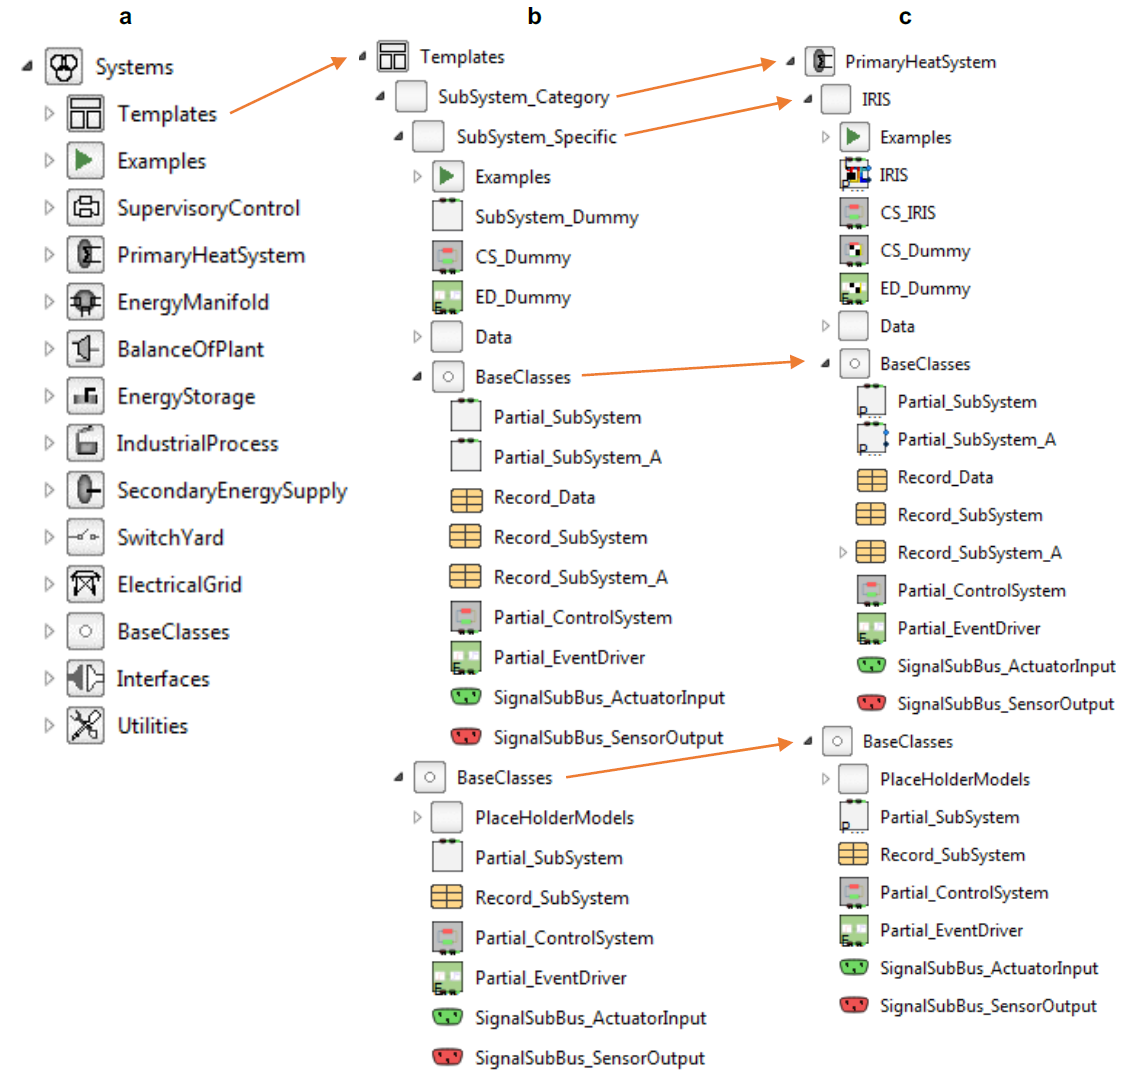
\includegraphics[width=\linewidth]{pics/Template System.png}
\caption{a) Overall Modelica package, b) template structure for creating new subsystem categories and specific subsystem models within a category,  c) example of a specific implementation of a primary heat system using the template approach. }
\label{fig:Template}
\end{figure}



\subsection{Understanding and Running Existing Models}

The hybrid repository is broken down using the templating system shown in Figure \ref{fig:Template}. 
The top level is the overall system package which incorporates all of the Modelica models contained within the NHES package. Then inside of the NHES package are the different subpackages (Systems, Electrical, Thermal, etc…). Within each of the subpackages are further subpackages as seen in the Systems package. Within the Systems package there are further subpackages called \textit{SubSystem Category} (Examples, PrimaryHeatSystem, EnergyStorage, etc…). Then within these SubSystem Categories there is yet another level of subpackage that is called \textit{SubSystem\textunderscore Specific}. Within the \textit{SubSystem\textunderscore Specific} category is where development takes place and potential configurations of the different processes take shape. Inside each SubSystem\textunderscore Specific there is a template that includes \textit{Examples}, \textit{Subsystem Dummy}, \textit{CS\textunderscore Dummy}, \textit{ED\textunderscore Dummy}, Data, BaseClasses, and usually a Components folder. For existing systems the Examples folder contains a runnable example the user can execute to see how the code runs at a top level and what scenarios it is capable of running. An example of which is depicted in Figure \ref{Example File}. For each example the user can double click on the main system which will open the table in the upper left hand corner of Figure \ref{Example File} which provides inputs for the user to change parameters about the system. Then if the user wishes to modify the control system utilized they can either choose from the drop-down menu, or click the button at the right of the “CS” line to open the table in the lower left hand section which provides options to delay when different control systems come online.  

\begin{figure}[hbtp]
\centering
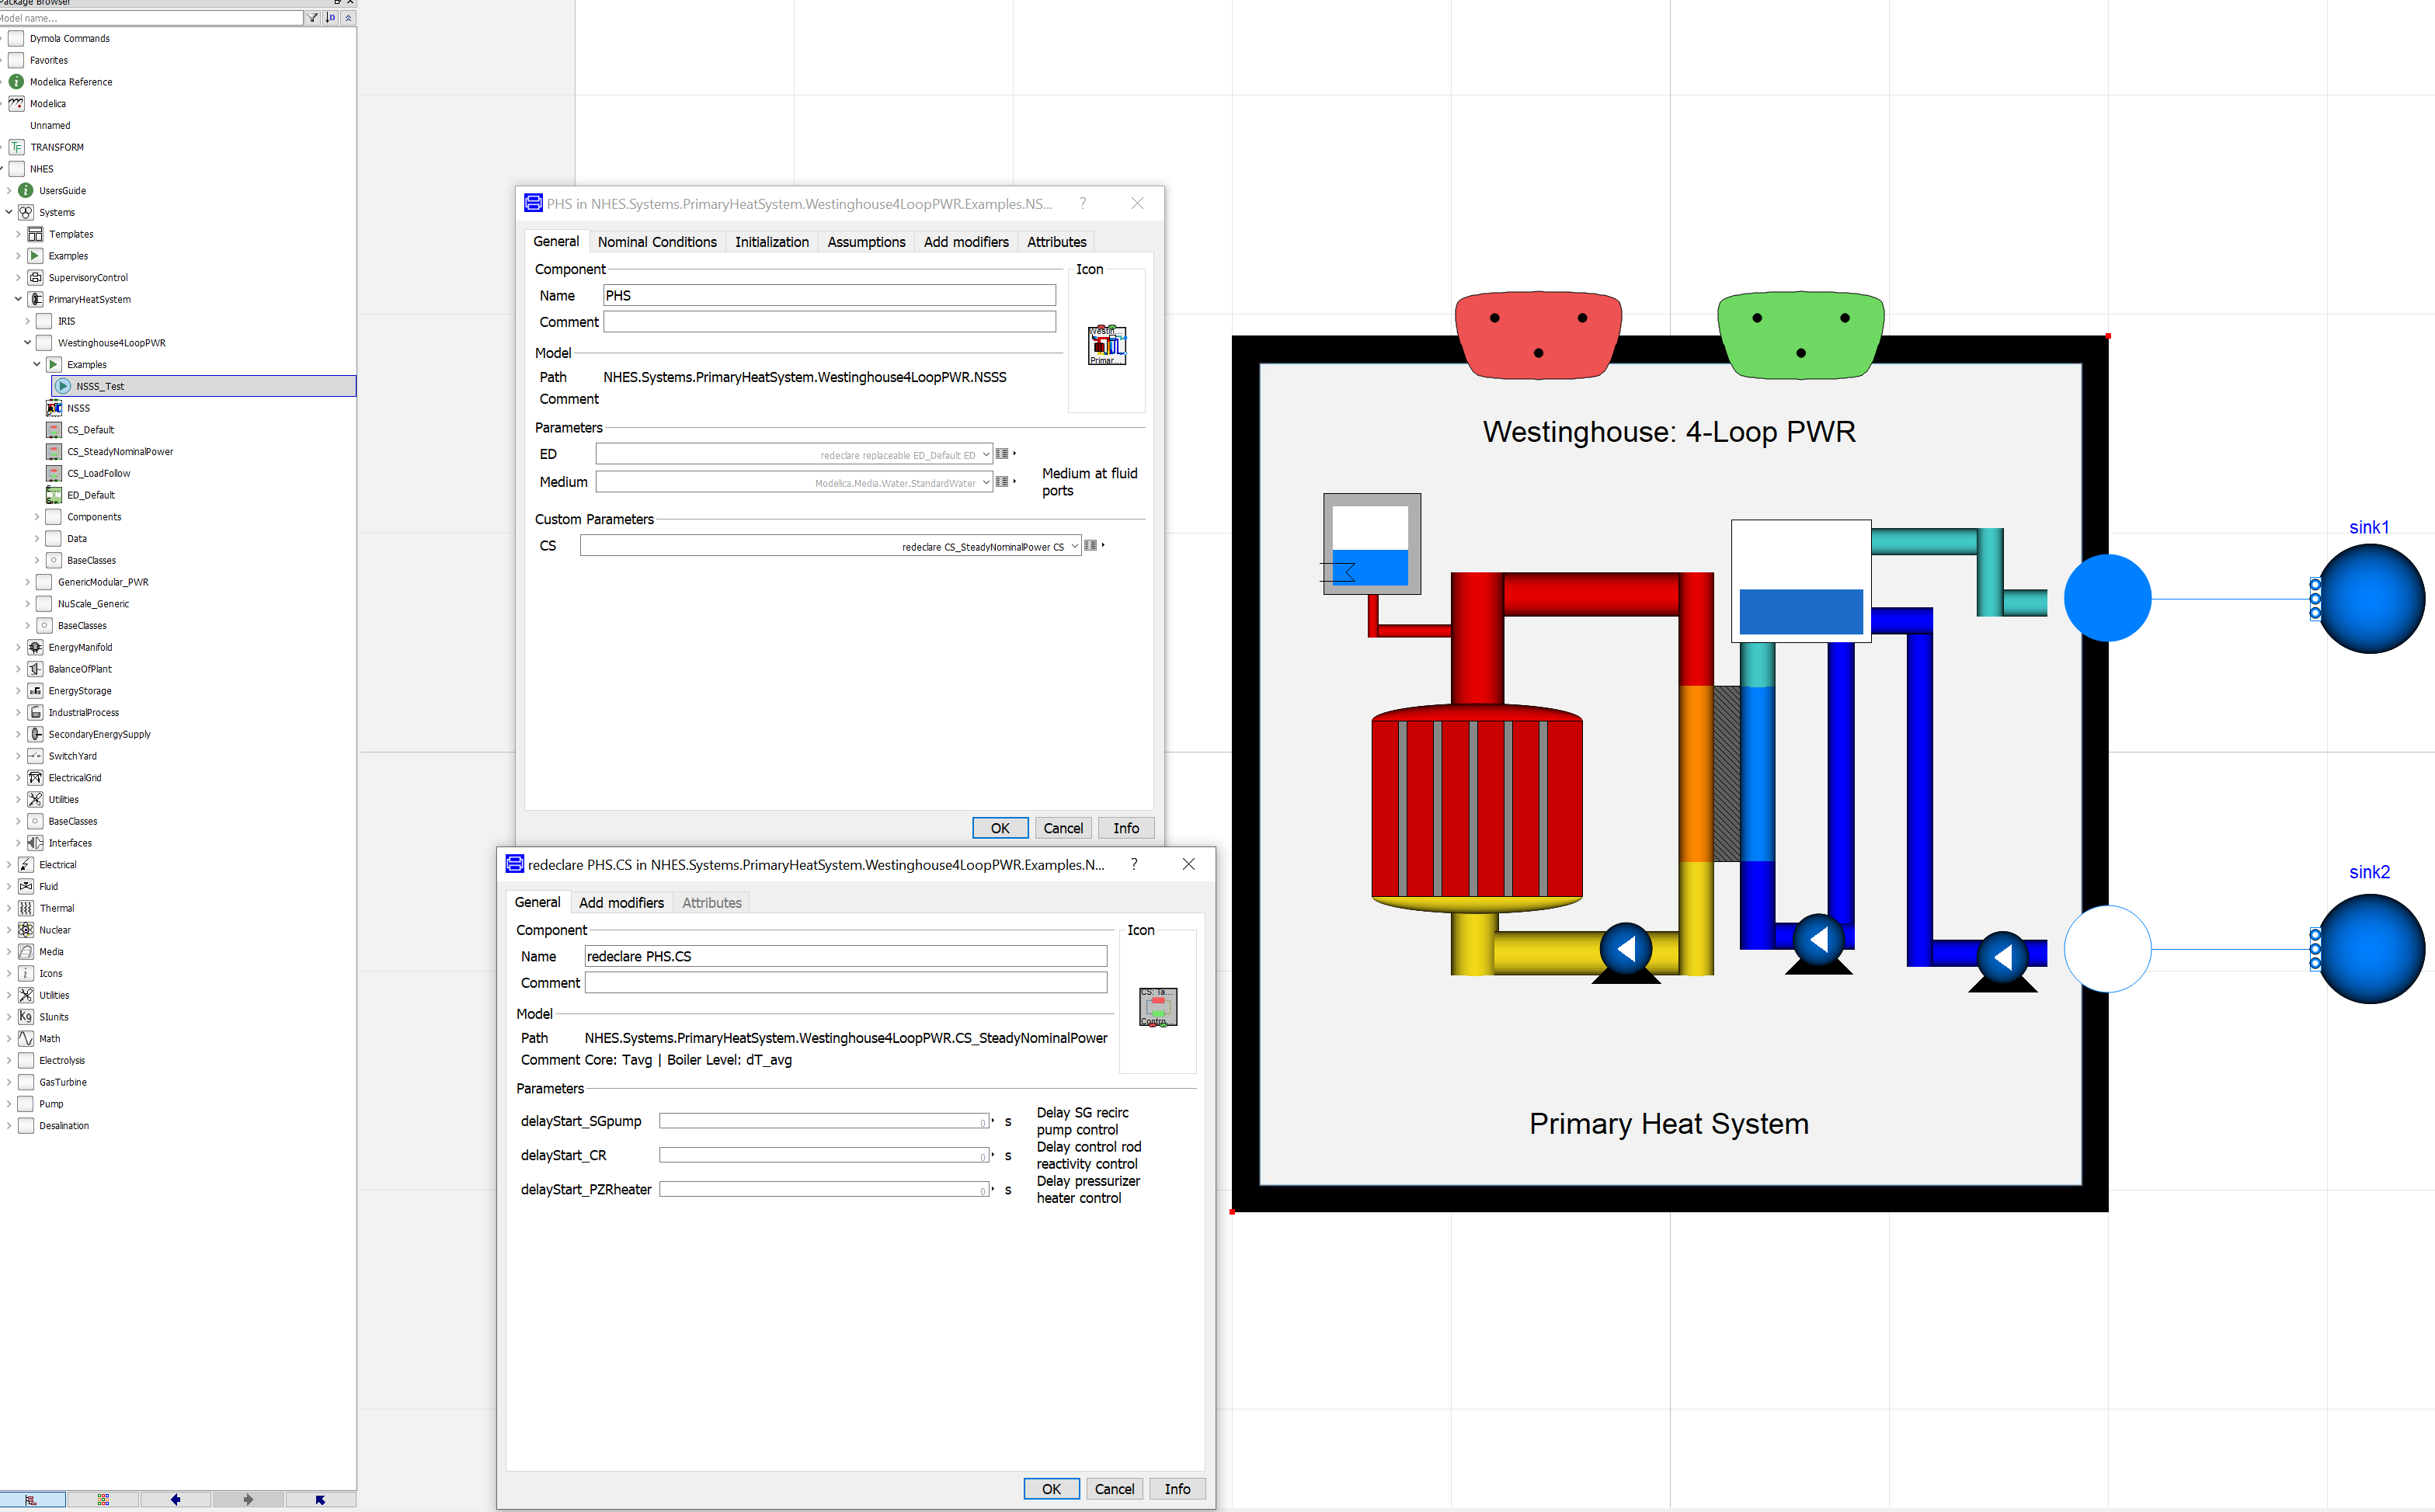
\includegraphics[width=\linewidth]{pics/Example_File.png}
\caption{Exploded view of the NSSS\textunderscore Test example within the NHES library with control system options opened up }
\label{Example File}
\end{figure}

These example tests provide a good way for the user to become associated with the large subsystem in terms of how they work and the different parameters that can be utilized to tune and interact with the models. In addition to the examples file a deeper understanding of the model can be realized by looking into the component structure of the model. This is typically accomplished through looking at the filled-out Subsystem Dummy section. For the Westinghouse 4-Loop plant this can be seen in Figure \ref{Westinghouse 4-loop}. This model includes several subcomponents connected into a singular model. Each model with its’ own set of parameters. Using this version of the model it is possible to discern the inner workings of the model in terms of sensors, physical descriptions of the code, inlet and outlet conditions, and system dependencies. 
In addition to the SubSystem Dummy section, large process models typically include a control system section which is created from the CS\textunderscore Dummy file in the branch. These control system files can be added as a control system for the Subsystem to control different valves, pumps, and control drives within the process from the dropdown menu in the “CS” section seen in Figure \ref{Example File}. large process systems may have several different potential control systems based upon what type of Integrated Energy System they are operating within. An illustration of one of the Westinghouse Control systems can be seen in Figure \ref{Control System}. 


\begin{figure}[hbtp]
\centering
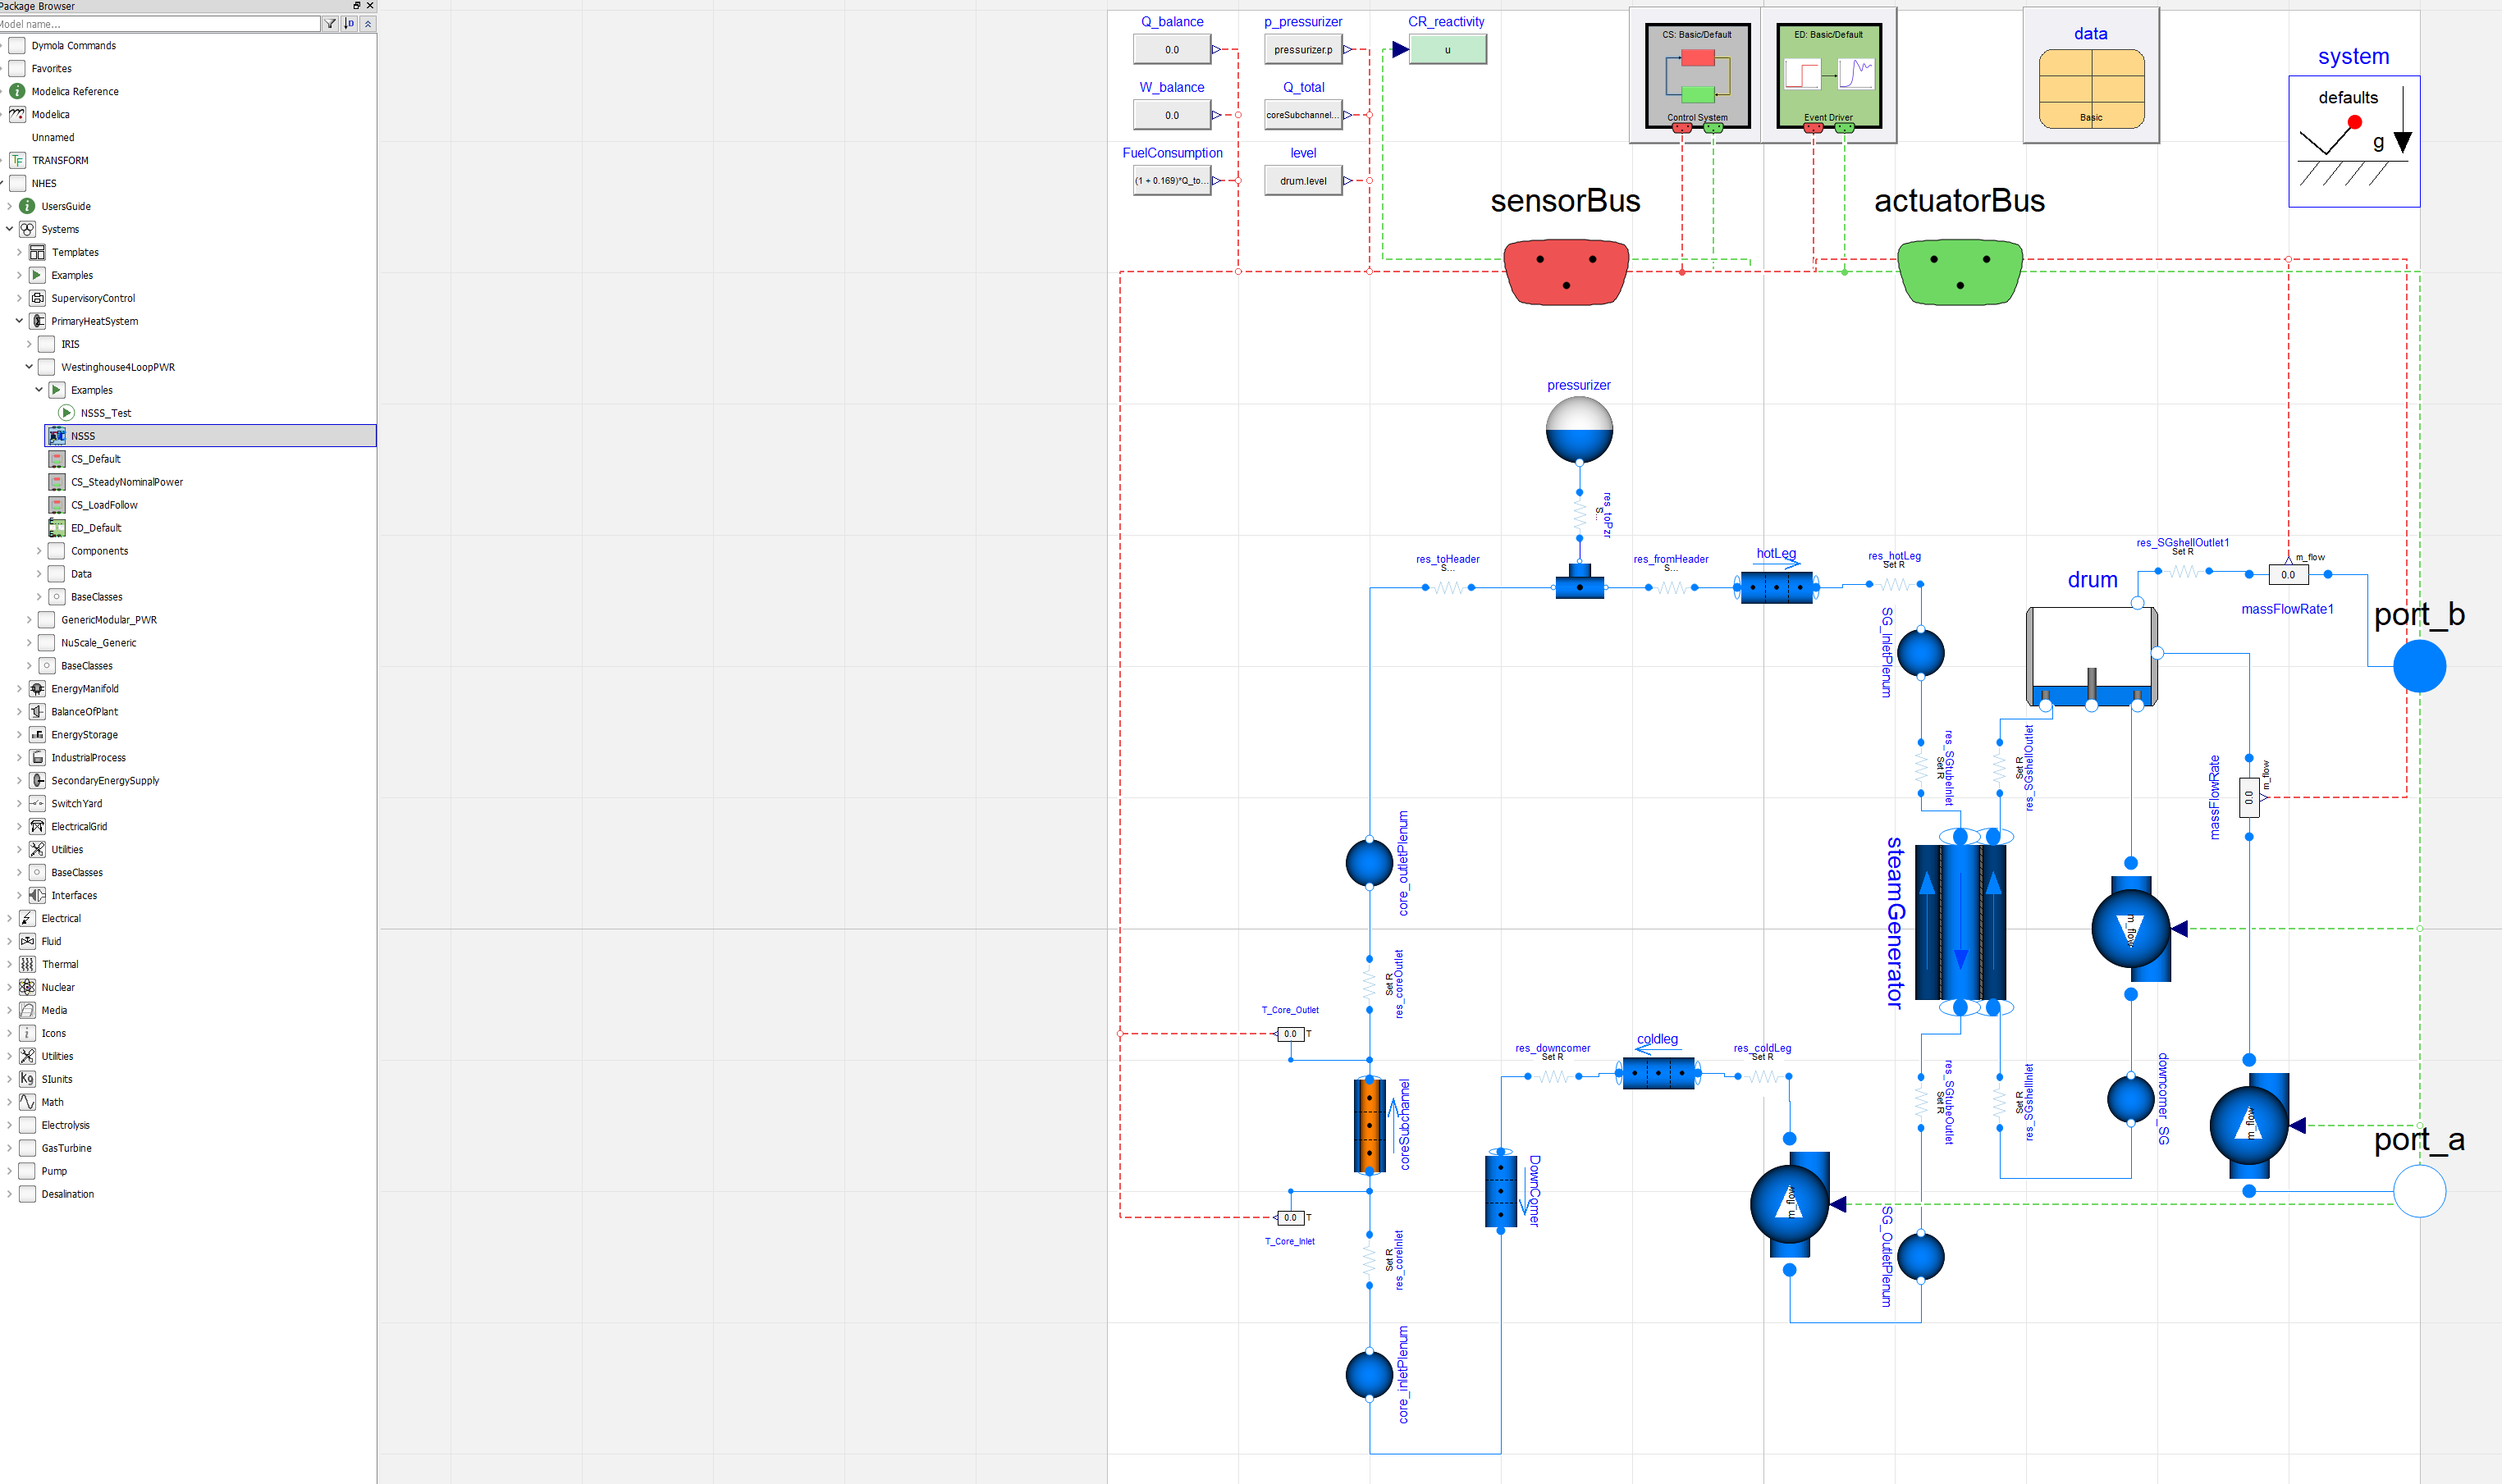
\includegraphics[width=\linewidth]{pics/Sub_System_Dummy.png}
\caption{Subsystem for the Westinghouse-4 Loop model.}
\label{Westinghouse 4-loop}
\end{figure}


\begin{figure}[hbtp]
\centering
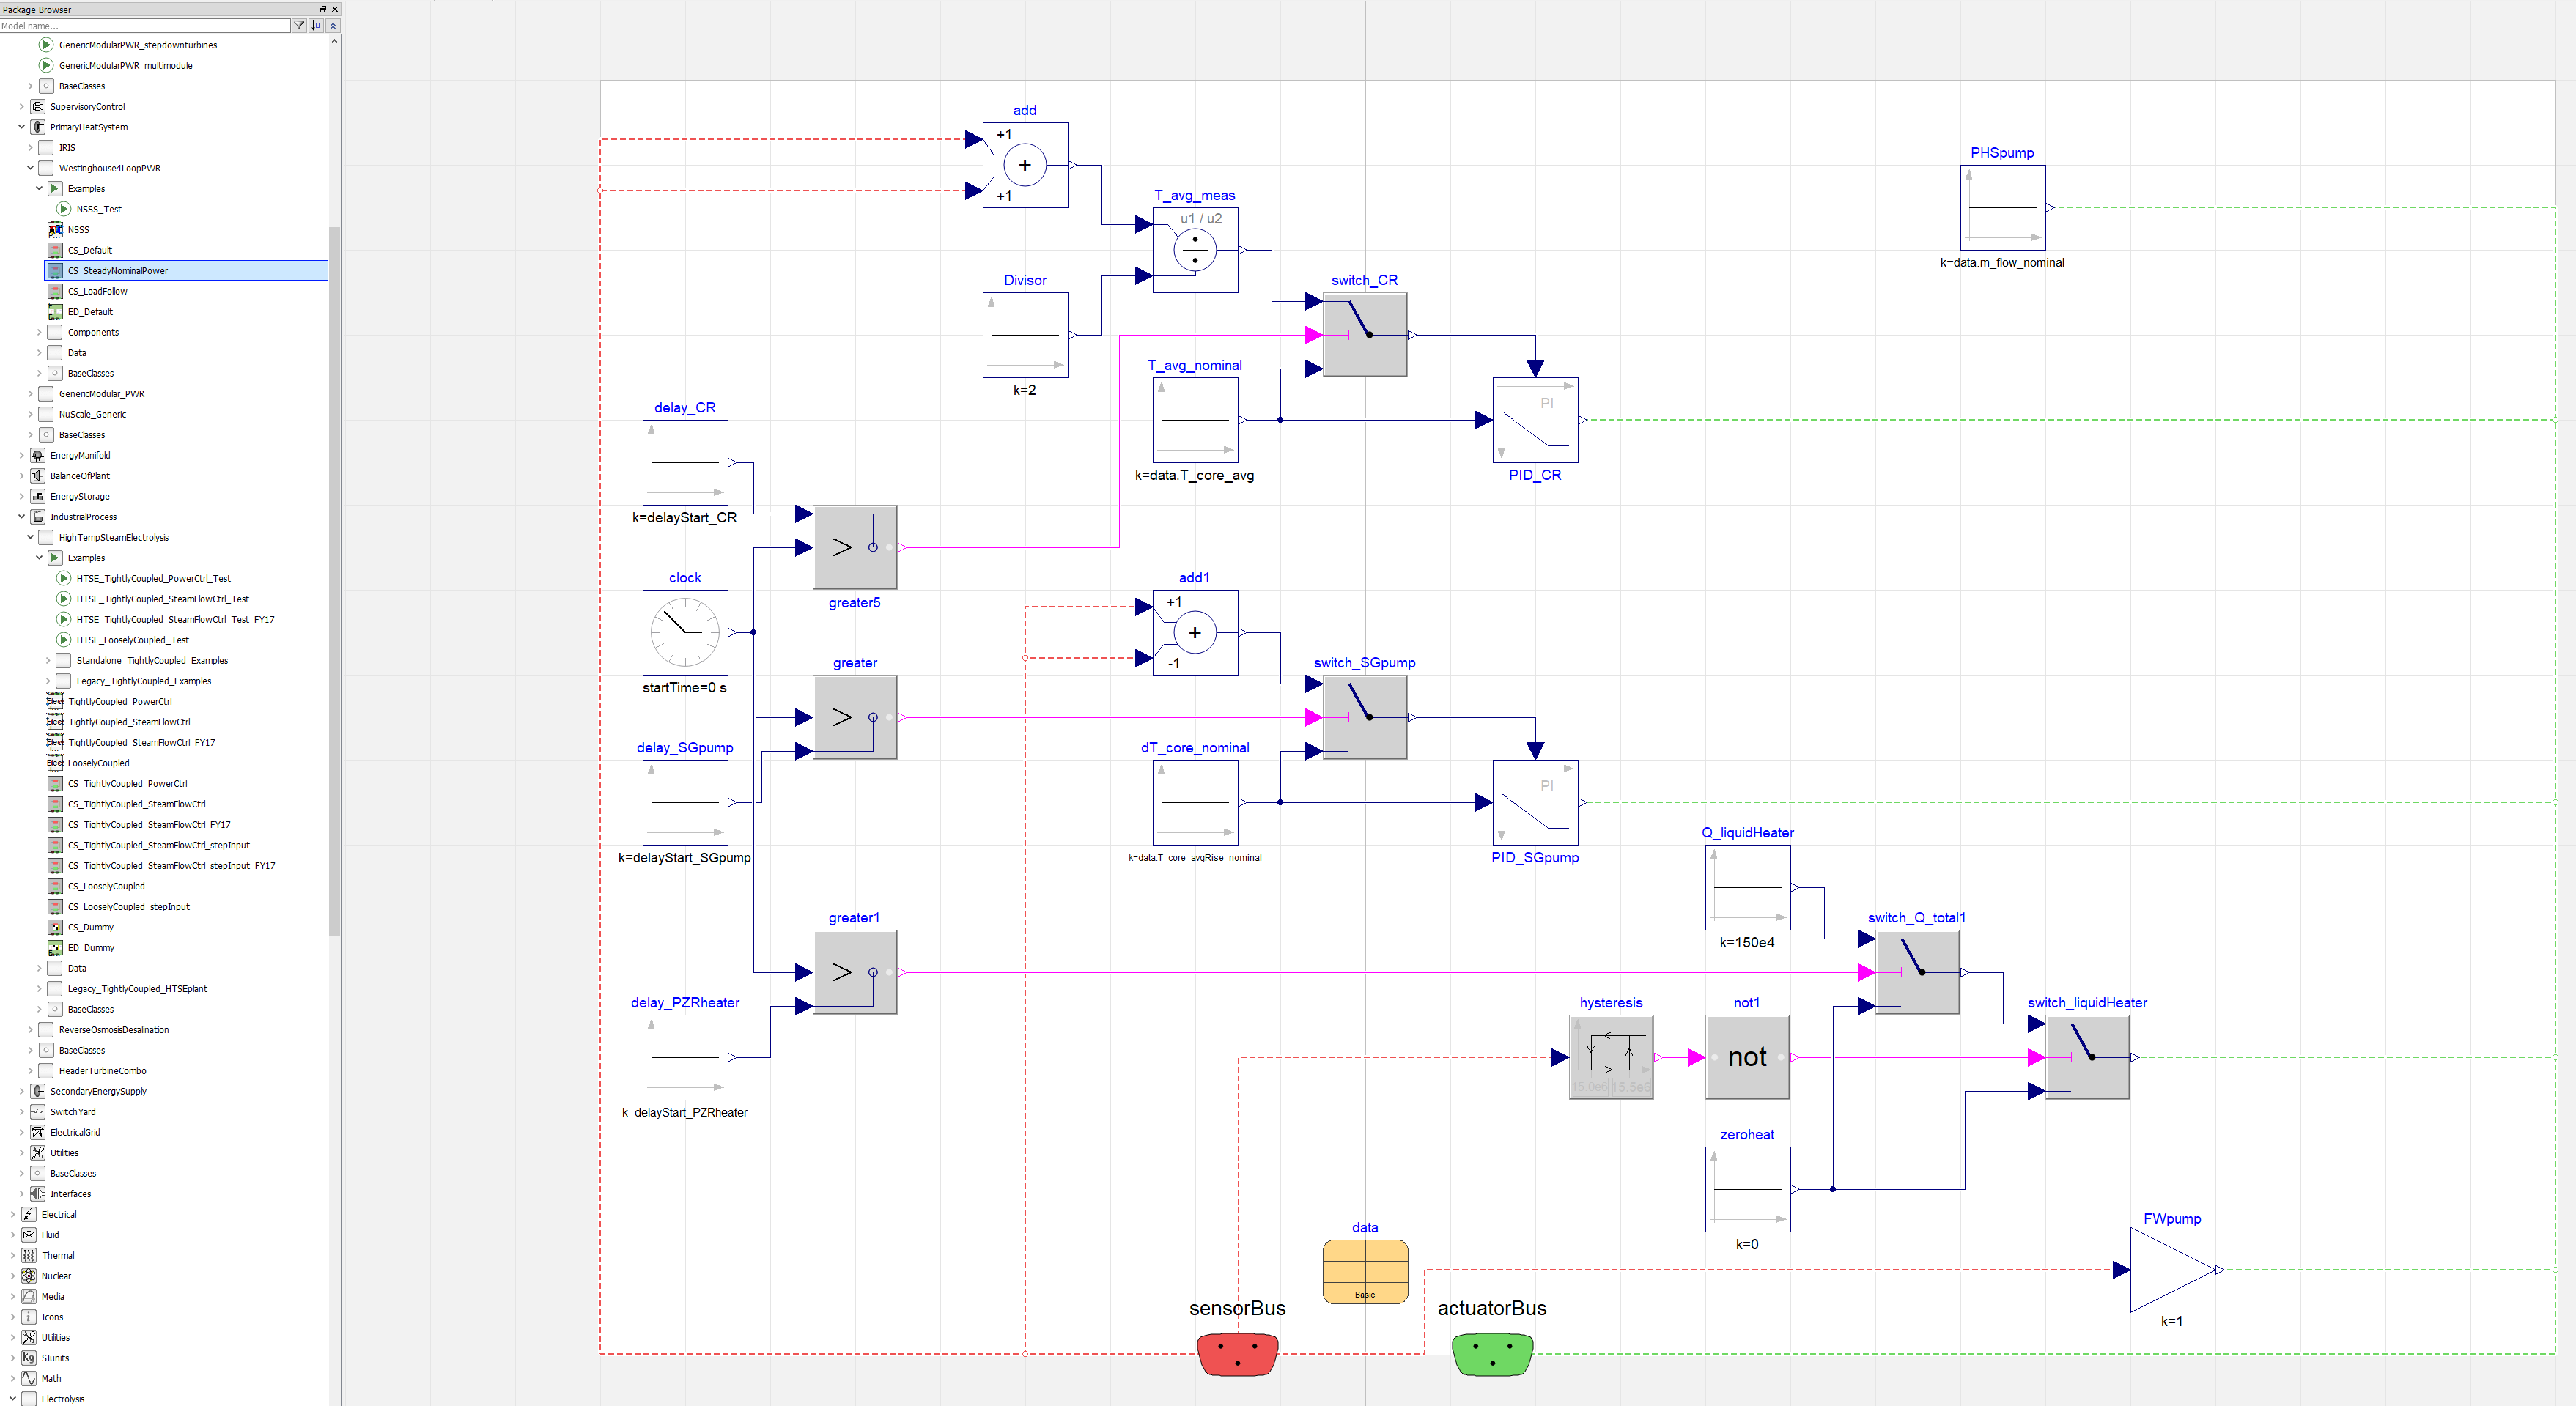
\includegraphics[width=\linewidth]{pics/Westinghouse_Control_picture.png}
\caption{Control System (CS) for the Westinghouse 4 Loop model}
\label{Control System}
\end{figure}

Assuming the user is creating a new package with new components specific to the model it is best to include those models with a “components” folder in the subpackage containing the “BaseClasses” folder. The Data folder is typically where the main data structures in terms of “records” of kept for the process model. Records are files that are intended to be used as an input deck to the main model for use as a set of “parameters” the components will read from. The ED\textunderscore dummy file within the \textit{Subsystem\textunderscore Specific} category is the Event Driver file and is rarely used and can be ignored from a user perspective.

\subsubsection{Modifying Existing Models for Specific Runs}
A starting point from which a user can begin model development and analysis is from an existing Example model. To properly edit the \textit{Examples} within the hybrid repository while still maintaining the regression system one needs to create a duplicate model of the example file that is to be edited. This can be done by right clicking on the file as shown below and creating a duplicate class.

\begin{figure}[hbtp]
\centering
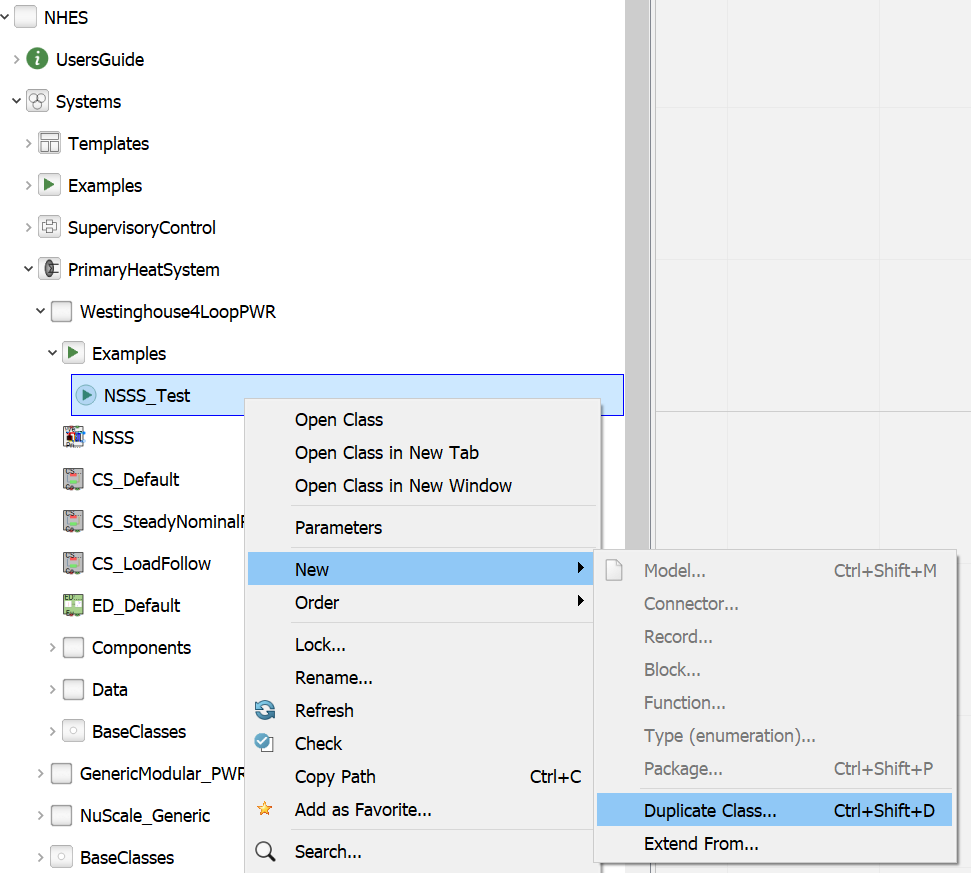
\includegraphics[width=\linewidth]{pics/DuplicateClass.png}
\caption{Creating a duplicate class for model runs.}
\label{Duplicate Class}
\end{figure}

This file will the be placed in the Examples folder where edits can be made to it for new and unique runs. This includes things such as new control schemes, sizing, timeruns, etc..

\subsection{Configuring Existing Models into Integrated Energy Systems}
Each subsystem of the Integrated Energy Systems is inherently interesting on its own and large spans of time can be spent researching and fine tuning them independently. However, the developer team is aware that in the evolving energy landscape, and to the extent users will come across this repository, that integrated energy systems are the primary focus.

This focus includes systems that involve the distribution of heat and electrical energy among several subsystems and the control schemes utilized to accomplish this. Therefore, this section seeks to provide an introductory understanding of how to connect subsystems together within the Hybrid repository. To accomplish this the NuScale\textunderscore Coupling\textunderscore Test Example will be created starting from the GenericModularPWR\textunderscore park system.

\begin{figure}[hbtp]
\centering
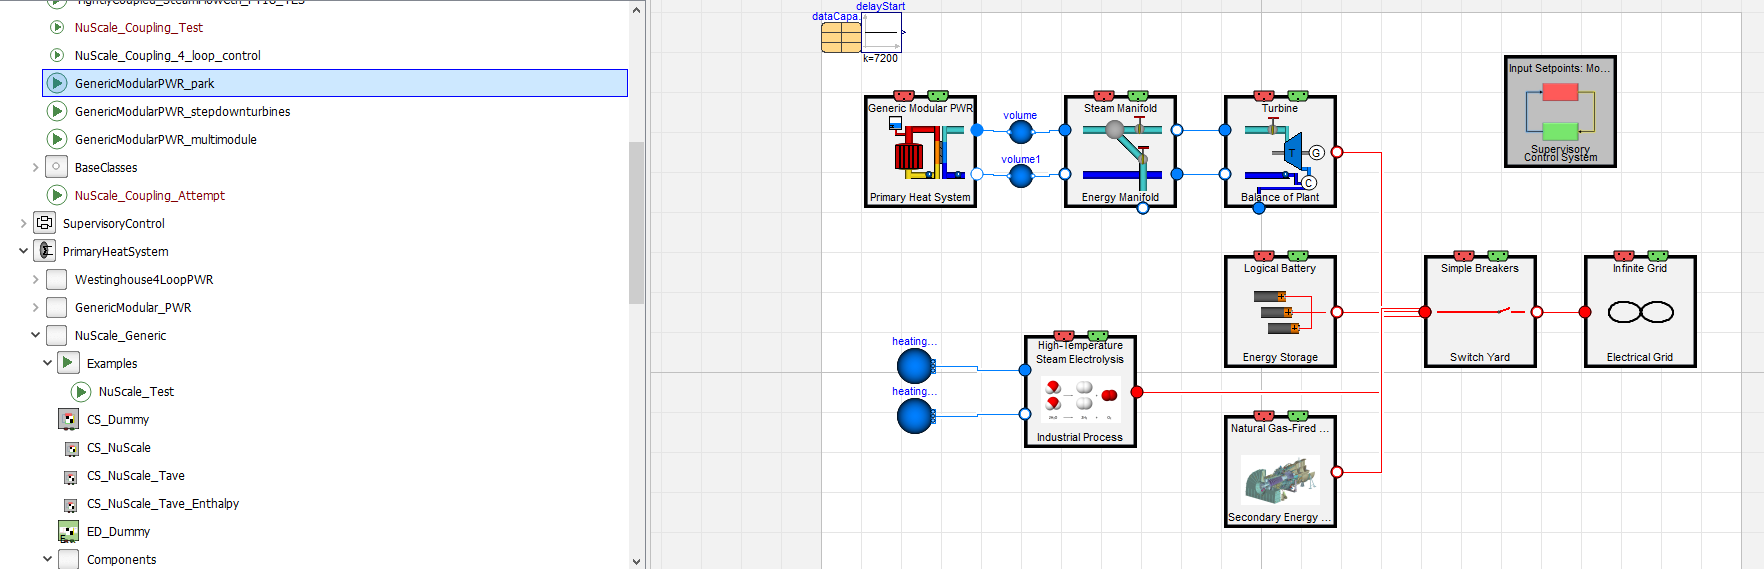
\includegraphics[width=\linewidth]{pics/Modular_Park_Start.png}
\caption{Initial Integrated Energy System Starting Point}
\label{modular park}
\end{figure}

The first step is to take a similar example that has the Supervisory Control System in the top level. In this case the GenericModularPWR\textunderscore park was used. A duplicate class was created and all the components aside the Steam Manifold, Turbine, Simple Breakers, infinite grid, supervisory control system, delay start, and data capacity were removed. See below.

\begin{figure}[hbtp]
\centering
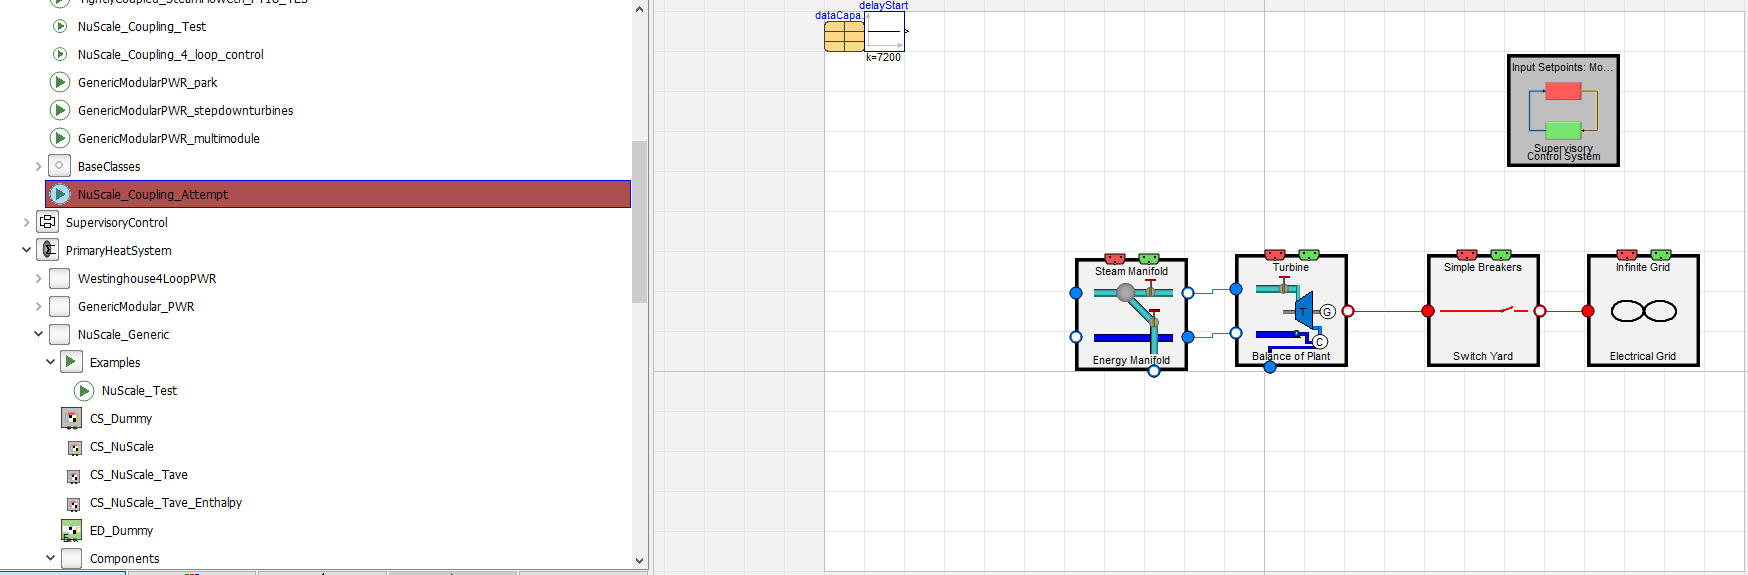
\includegraphics[width=\linewidth]{pics/CouplingCreation.png}
\caption{Rearrangement of Initial Energy System}
\label{coupling park}
\end{figure}

Then the primary side of the NuScale was added in this case the \textit{NuScale\textunderscore Taveprogram} version of the NuScale primary unit.

\begin{figure}[hbtp]
\centering
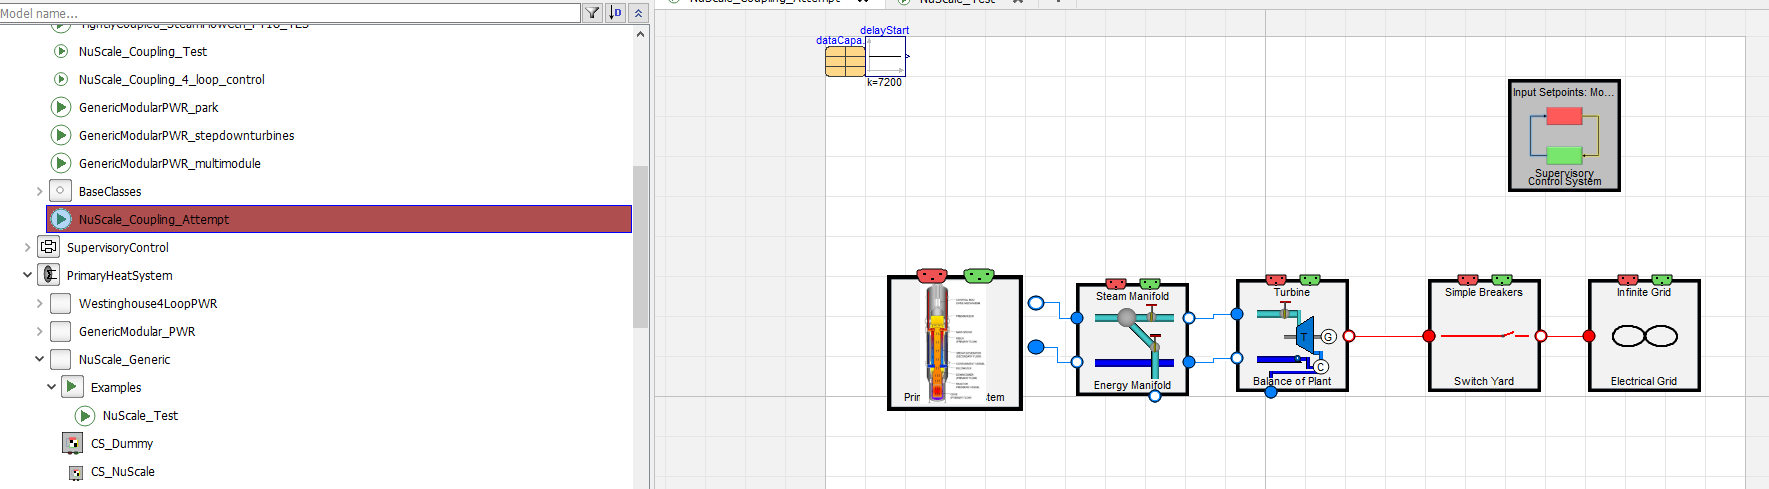
\includegraphics[width=\linewidth]{pics/CouplingCreation_2.png}
\caption{Creation of NuScale Energy System}
\label{NuScale park}
\end{figure}

Then from this point it is a matter of telling the systems what control schemes to use. For this system the reactor operates to meet a certain primary system average temperature in accordance with the turbine output. To input this the control system: PrimaryHeatSystem.NuScaleGeneric.\\ CS\textunderscore NuScale\textunderscore Tave was used with input:
W\textunderscore turbine = BOP.powerSensor.power and W\textunderscore Setpoint  =  SC.W\textunderscore totalSetpoint\textunderscore BOP, see Figure \ref{primary controller settings}.  And the turbine control scheme is modified to reflect a once through system type control strategy where the turbine control valve operates to meet a constant pressure in the turbine, Figure \ref{Turbine Control Settings}. While it is noted that is not the official control strategy strictly speaking for the NuScale system nor is it the one used in load following scenarios in the hybrid repository, it does provide a baseline for which to control the system and modifications can be made from this point.  The power setpoints in the BalanceOfPlant.Turbine.CS\textunderscore OTSG\textunderscore Pressure control module are 160MW for both Reactor\textunderscore Power and Nominal\textunderscore Power while p\textunderscore nominal parameter is set to BOP.port\textunderscore a\textunderscore nominal.p to ensure a single parameter value is carried throughout the system. Additionally, W\textunderscore totalSetpoint is set to SC.W\textunderscore totalSetpoint\textunderscore BOP, Figure \ref{Turbine Control Settings}.

\begin{figure}[hbtp]
\centering
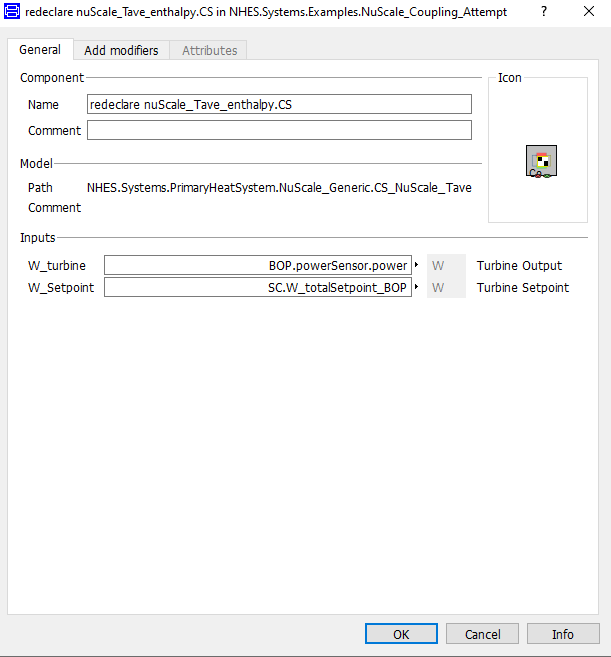
\includegraphics[width=\linewidth]{pics/primary_controller_settings.png}
\caption{Primary System Controller Settings}
\label{primary controller settings}
\end{figure}


\begin{figure}[hbtp]
\centering
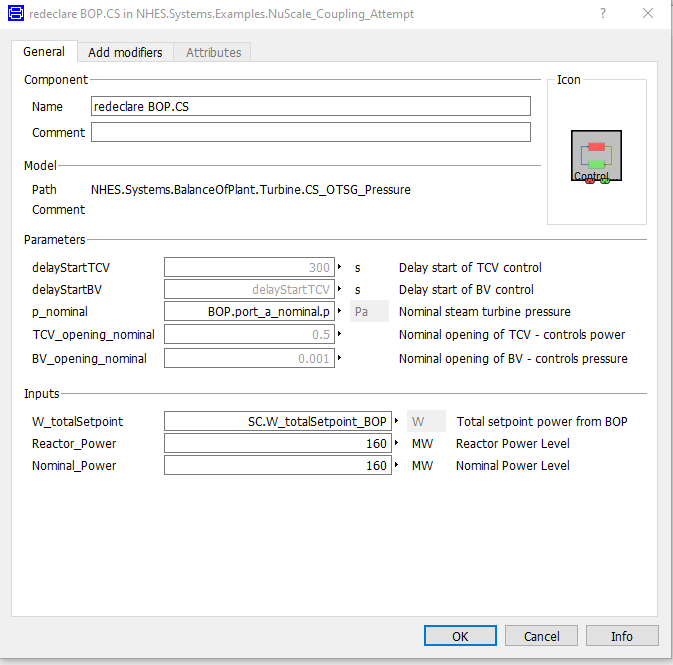
\includegraphics[width=\linewidth]{pics/BOP_settings.png}
\caption{Turbine Control Settings}
\label{Turbine Control Settings}
\end{figure}

To complete the construction of the model the systems need to match on the boundaries.  To do this the values from the primary heat system need to be transferred to the Steam Manifold under the nominal values tab, Figure \ref{Port a Nominal Values} and \ref{port B Nominal Values}.

\begin{figure}[hbtp]
\centering
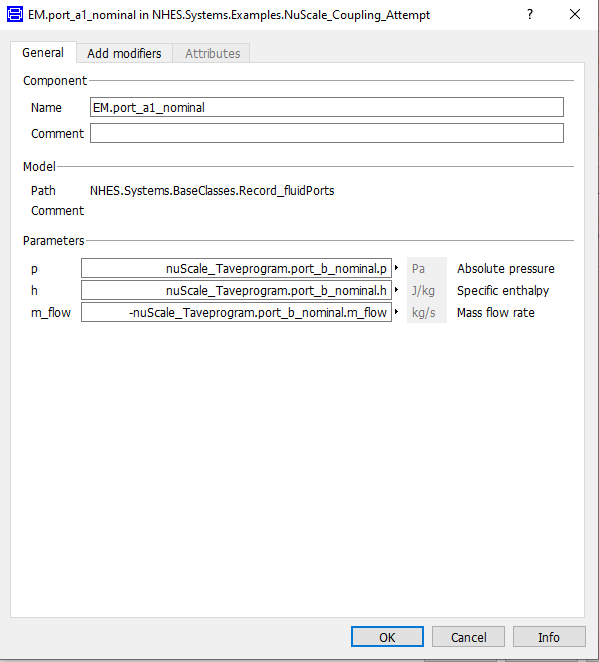
\includegraphics[width=\linewidth]{pics/Nominal_Values_BOP.png}
\caption{Port a Boundary Values of the Energy Manifold}
\label{Port a Nominal Values}
\end{figure}

\begin{figure}[hbtp]
\centering
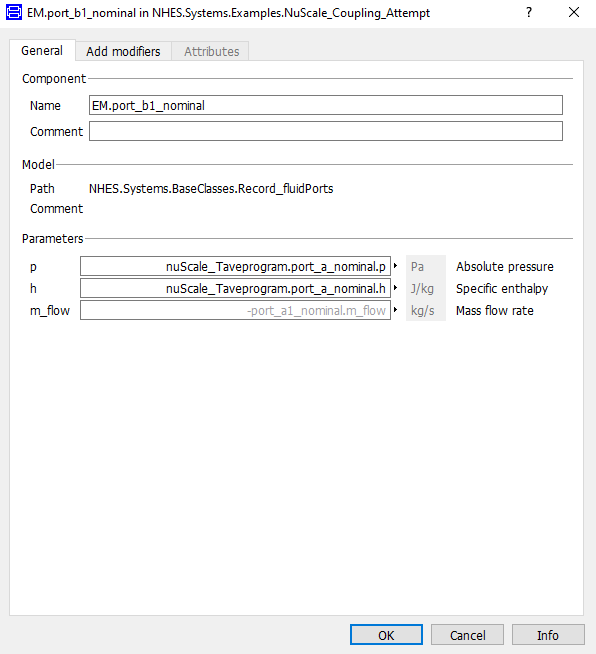
\includegraphics[width=\linewidth]{pics/Manifold_Nominal_b.png}
\caption{Port b Nominal Values of the Energy Manifold }
\label{port B Nominal Values}
\end{figure}

\subsection{Test Creation}
To create a regression test once a user develops an example test in the Dymola NHES library can be accomplished through a couple of settings. In the Dymola simulation setup tab in the output tab uncheck the store at variable events box. Then click store in model button and check the output box, click ok, then click ok again, then Save the model. Example settings are shown in Figure \ref{mat file settings}.


%\begin{figure}[hbtp]
%\caption{dfgsg}
%\centering
%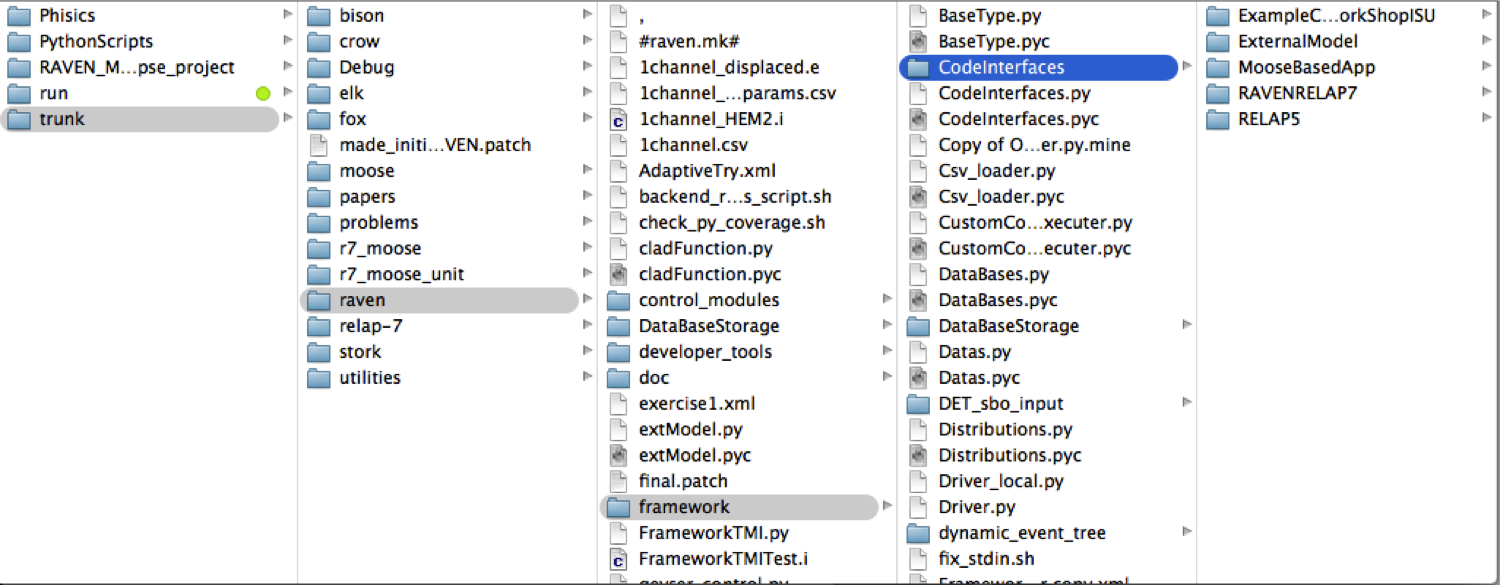
\includegraphics[width=\linewidth]{pics/CodeInterfaceLocation.png}
%\end{figure}


\begin{figure}[hbtp]
\centering
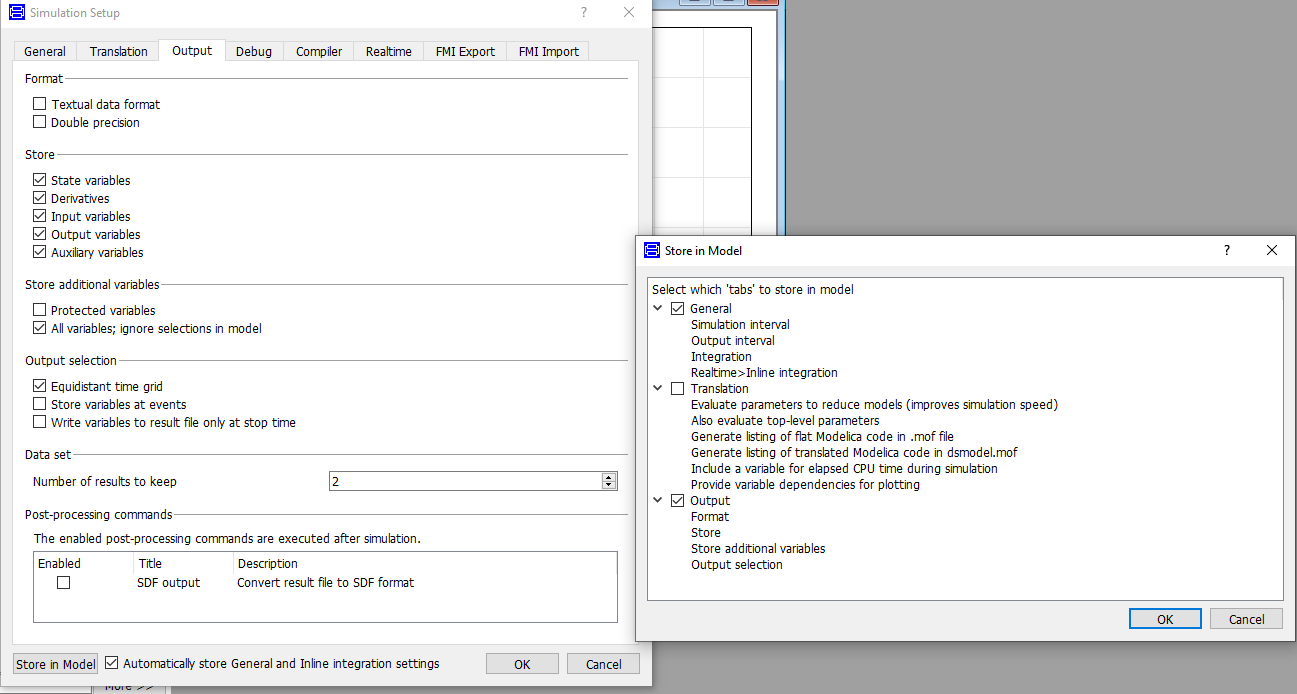
\includegraphics[width=\linewidth]{pics/Test_Creation.png}
\caption{Settings to Create a proper mat file for a gold folder test}
\label{mat file settings}
\end{figure}
In the simulateModel command one of the following two flags is required. Either "\textit{numberOfIntervals}" or "\textit{OutputInterval}". numberOfIntervals tells dymola how many output intervals to make. OutputInterval tells dymola at what timestep interval should an output be present for comparison. The .mat file in the gold folder will need to be run using the same simulateModel command that is present in the .mos file being created.

These can be selected in the Simulation Setup tab of the Dymola GUI, Figure \ref{Interval Setup}, and should carry down to the command you copy and paste in the .mos file. An example is shown below of the simulation setup tab.

\begin{figure}[hbtp]
\centering
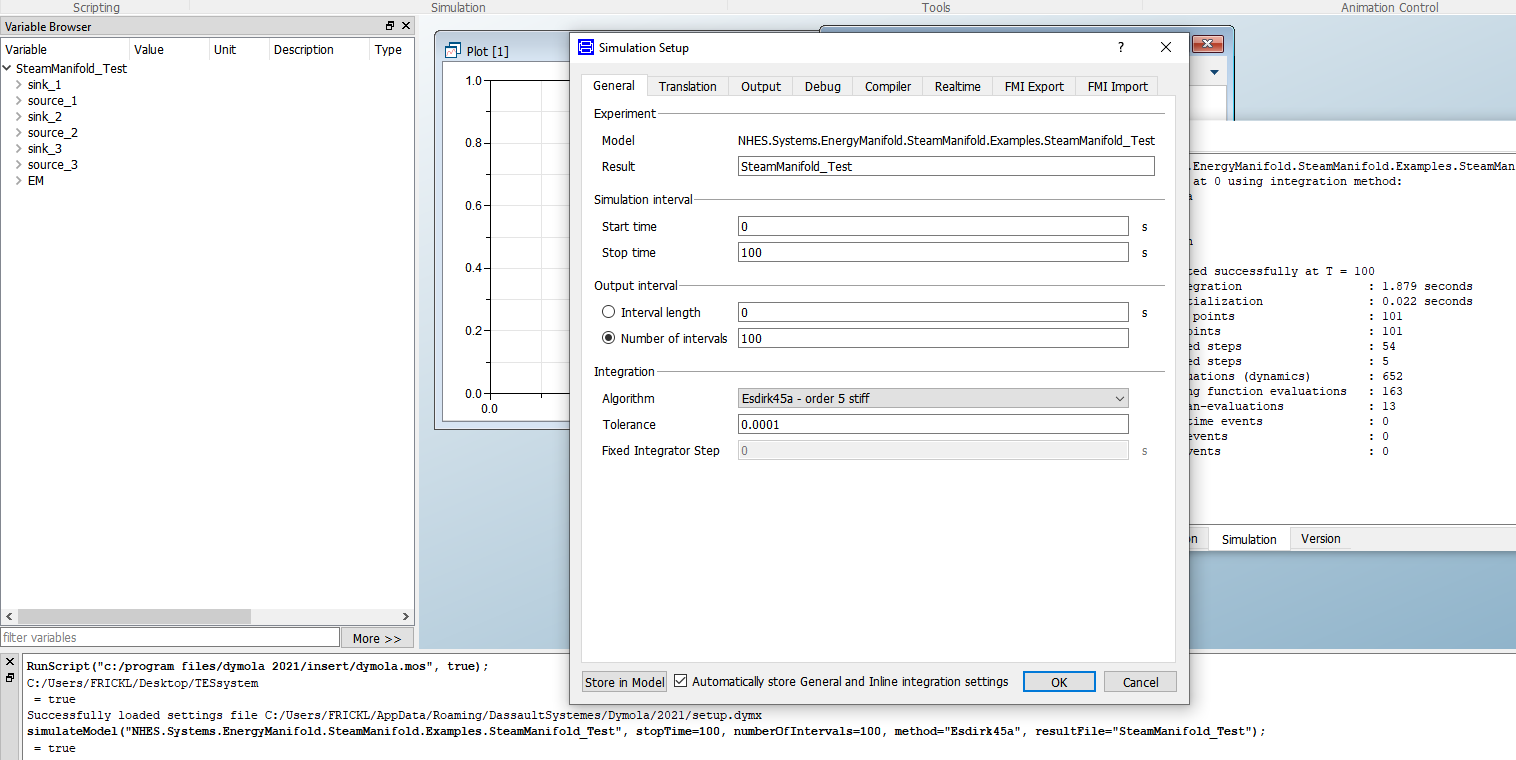
\includegraphics[width=\linewidth]{pics/Regression_picture.png}
\caption{Simulation Setup}
\label{Interval Setup}
\end{figure}

Then run the simulation, (ideally a test should take less than 100 seconds). On the simulation tab in the command line copy the simulation command. Example below:

\begin{lstlisting}[language=bash, basicstyle=\small]
simulateModel("NHES.Systems.EnergyManifold.SteamManifold.
Examples.SteamManifold_Test", stopTime=100, numberOfIntervals=100,
method="Esdirk45a", resultFile="SteamManifold_Test");
\end{lstlisting}

This command should then be added to a file and named something like Test\textunderscore Example.mos. The command can be found in the Simulation Setup tab of the Dymola GUI once you hit simulate

Then in folder /path/to/hybrid/hybrid/tests/dymola\textunderscore tests create a folder named Test\textunderscore YourModel.

Create a \textit{gold} folder in the new folder, drop the .mat file from your simulation that is named resultFile="SteamManifold\textunderscore Test" from your simulateModel command into the gold folder. The .mat file is created in your working directory in Dymola. Then in the main Test\textunderscore YourModel folder drop the Test\textunderscore Example.mos file and create a tests file open it up and place the following in it:


\begin{lstlisting}[language=bash, basicstyle=\small]
[Tests]
 [./]
  type = 'HYBRIDTester'
  input = 'Test_Example.mos'
  workingDir = '.'
  output = 'SteamManifold_Test.mat'
  dymola_mats = 'SteamManifold_Test.mat'  
  rel_err = 0.001
 [../]
[]
\end{lstlisting}

where SteamManifold\textunderscore Test.mat should be your result .mat file name, rel\textunderscore error is the amount of error allowed between the gold file and the regression test output, and Test\textunderscore Example.mos is the run script created.

\subsection{Advanced Test File Options utilized for complex models}
For complex models the initialization phase of a simulation can take the Modelica solvers a significant amount of time to find an initialization point. This occurs due to the highly nonlinear nature of the underlying physical equations.  A way to avoid such situations is to provide a restart file to bypass the initialization phase of the simulation. A restart file is automatically created at the end of each simulation as the dsfin.txt file created in the folder where the simulation is run. This file includes the final values of the previous simulation from which the new model can restart.   Move this file to the gold folder for your new testing system.
Once this file is created it can then be loaded automatically via the continue button in Modelica under the Simulation Tab. Select $Continue \rightarrow  Import Initial  \rightarrow  dsfin.txt  $. See Figure \ref{import Initial}.

\begin{figure}[hbtp]
\centering
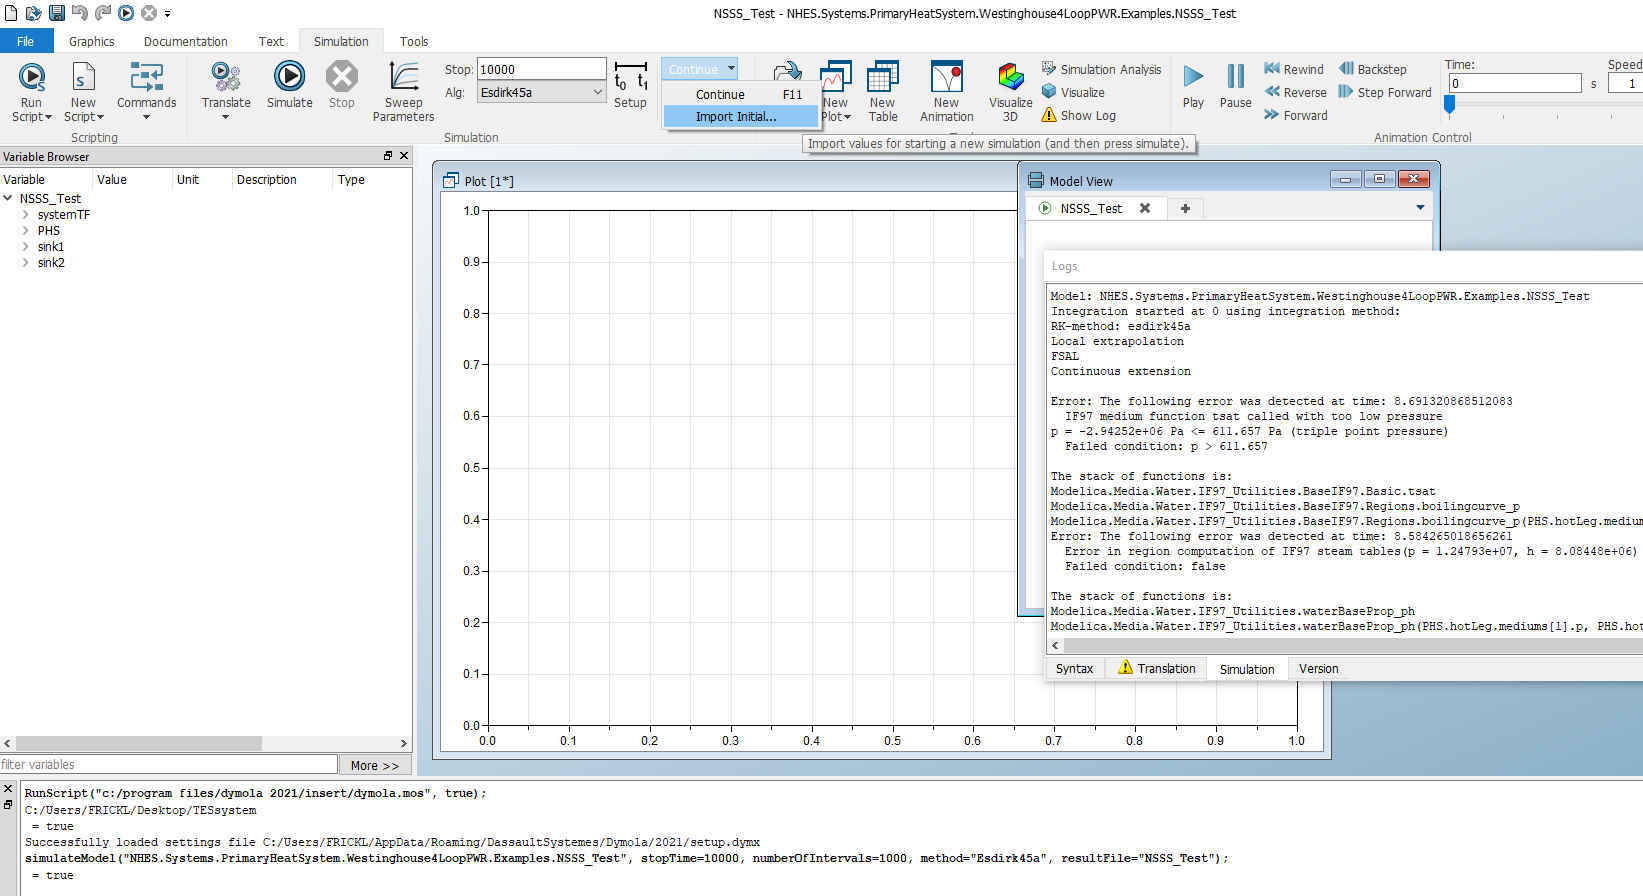
\includegraphics[width=\linewidth]{pics/Import_Initial.png}
\caption{Import Initial conditions from a previously run simulation}
\label{import Initial}
\end{figure}

Then once the dsfin.txt file is loaded go into the Setup tab and move the time back to start from zero and the end time to the desired simulation point for the test, shown in Figure \ref{Simulation Time Realignment}. This is necessary since Dymola assumes the user wants to restart the simulation from where it ended in time as well. This is not the case for the test. Instead the goal is to skip the initialization phase of the simulation and provide a clean solution with which to compare.

\begin{figure}[hbtp]
\centering
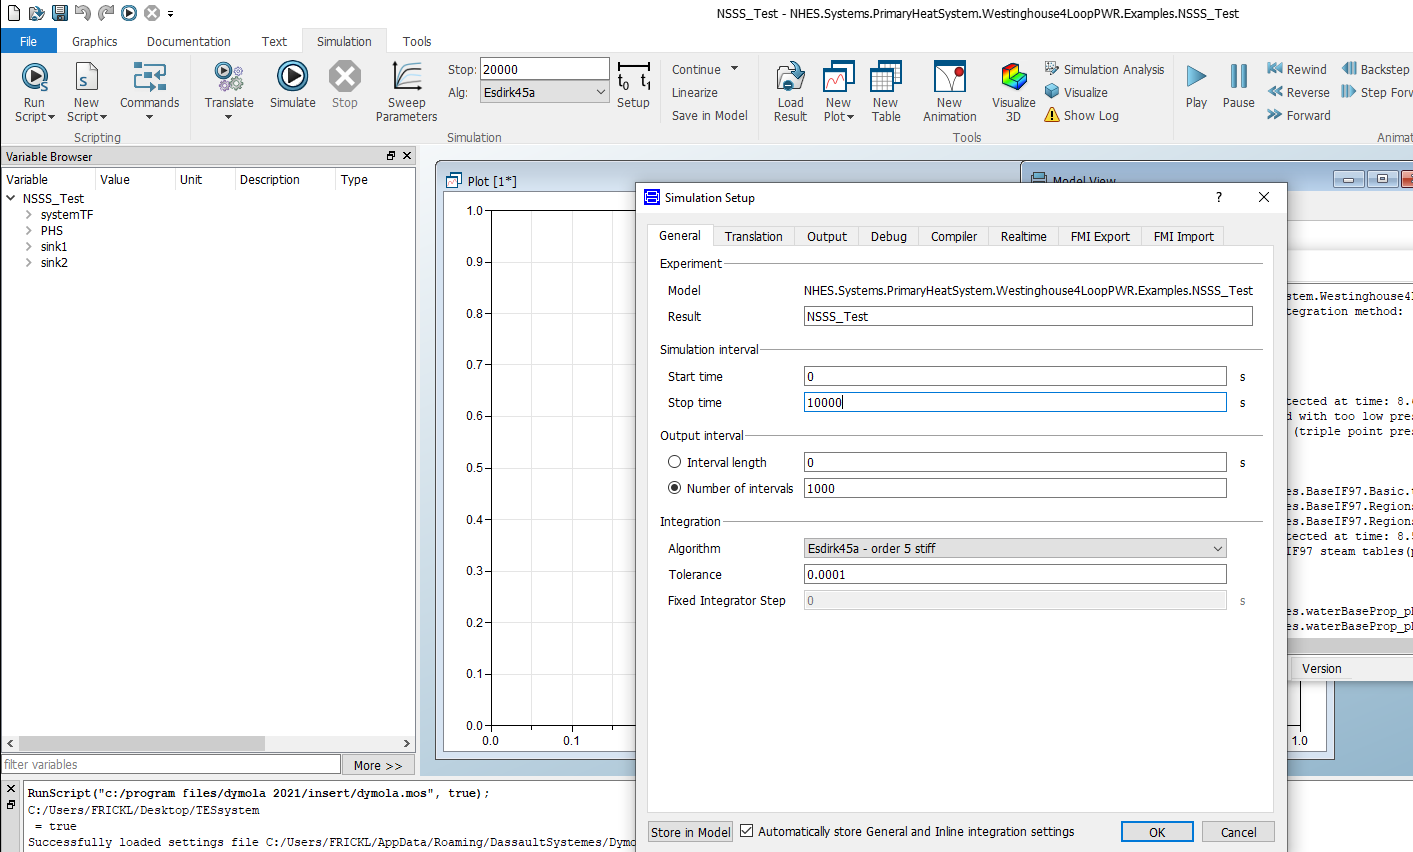
\includegraphics[width=\linewidth]{pics/Move_back_time.png}
\caption{Realign the Simulation Time}
\label{Simulation Time Realignment}
\end{figure}

Simulate this model and save the result file, in this example “NSSS\textunderscore Test.mat” and place it into the gold folder of the testing system. Additionally, copy and paste the simulateModel command that is in the Dymola GUI as the last line of your .mos script file for the test. The first two lines should be translateModel to make sure the right model is loaded into the equation set, followed by the importInitial command that loads all the values into the translated Model. The final command should be the simulateModel command.
The .mos file should look something like what is shown below.

\begin{lstlisting}[language=bash, basicstyle=\small]
translateModel("NHES.Systems.PrimaryHeatSystem.Westinghouse4LoopPWR
.Examples.NSSS_Test");

importInitial("./gold/dsfinal.txt");

simulateModel("NHES.Systems.PrimaryHeatSystem.Westinghouse4LoopPWR.
Examples.NSSS_Test", stopTime=10000, numberOfIntervals=250,
method="Esdirk45a", resultFile="NSSS_Test");
\end{lstlisting}
% definitions

% content
\section{Model Description}
It is the intent of this document to provide a level of understanding of each of the process models sufficient to allow users, with some background of Modelica, the ability to integrate, modify top level parameters, and run simulations of Integrated Energy Systems. Advanced users will be able to use the models as they see fit, but the descriptions provided here will not necessarily explain all facets of the models in detail. 

\subsection{Primary Heat System}
In the Hybrid repository there are four potential primary heat sources: The  Four-Loop PWR plant, the Generic Modular PWR, a natural circulation SMR power plant, and the Natural Gas Fired Turbine. Generally, we consider the Natural Gas Fired Turbine as a peaker unit and thus will save its’ discussion and coverage for the secondary power source section of the Model Descriptions.

\subsubsection{Four Loop Pressurized Water Reactor}

The Four loop PWR system, Figure \ref{Top View Westinghouse}, is designed to be consistent with publicly available information for the Westinghouse plant design \cite{Westinghouse}. This is a Pressurized Water reactor with a nominal thermal power of 3400MWt and has control systems designed to output 1100MWe. All system parameters can be found in the SubSystem model under the “data” record. The steam generator is of U-tube design and operates at a nominal pressure 1000psia. Reactivity feedback can be found in the coreSubchannel module alongside an external source of activity that is designed to provide reactivity feedback from the control rods. Reactivity in the core is based on a point kinetics models, that includes feedback from fission products, boron, fuel temperature, and moderator temperature. System decay heat is calculated from the TRANSFORM package via an eleven-group decay heat correlation from the TRACE user manual.

\begin{figure}[hbtp]
\centering
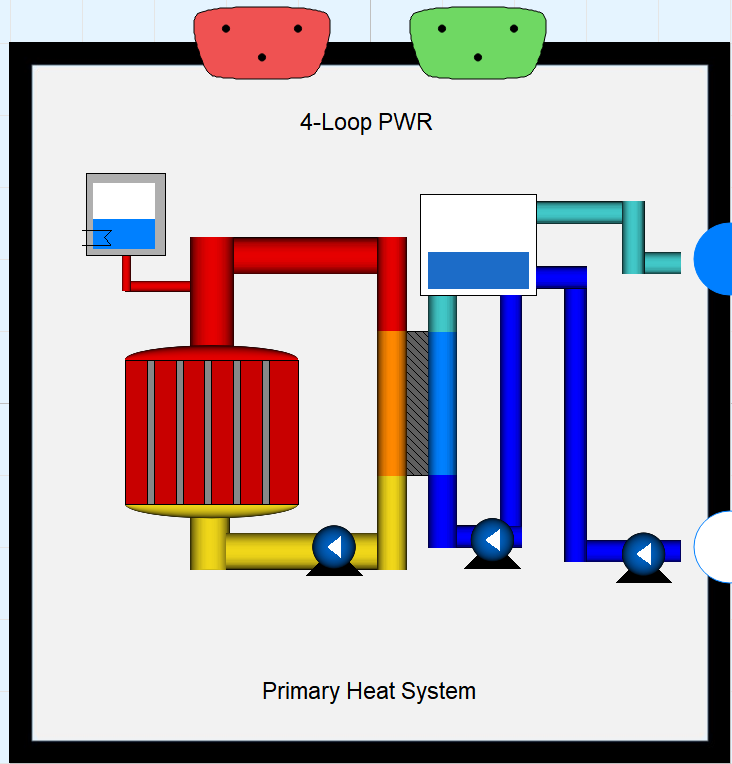
\includegraphics[scale=0.3]{pics/Westinghouse.png}
\caption{Top View of the Four-Loop PWR Plant}
\label{Top View Westinghouse}
\end{figure}


\subsubsection{Generic Modular PWR}
The generic modular PWR unit, Figure \ref{Top View Generic Modular}, is sized to be 160 MWt with 50MWe output as is consistent with the NuScale power module. However, the generic modular PWR does not operate under natural circulation but instead operates under forced flow. Therefore, this unit provides more stability in the code since it does not rely on density differentials to drive flow. This makes the unit less useful than is the NuScale style reactor modeled below, but it does provide the user a power input consistent with NuScale style systems but without the need to tune system geometries, friction factors, etc.. to meet the proper flow dynamics. As with the Westinghouse plant the data file is included in the subsystem  model and has reactivity controls within the core submodule. The Generic Modular PWR relies heavily on the TRANSFORM library for its subcomponents. The steam generator is a once through design with geometrical orientation consistent with a helical coil steam generator. 

\begin{figure}[hbtp]
\centering
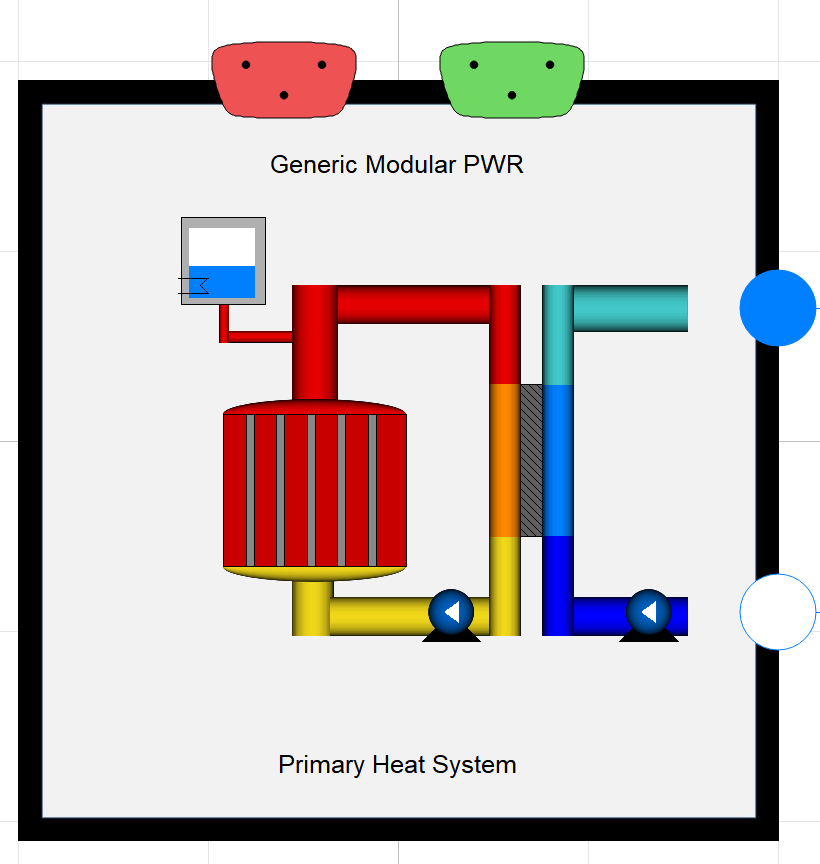
\includegraphics[scale=0.3]{pics/Generic_Modular_PWR.png}
\caption{Top Level Depiction of the Generic Modular PWR in the NHES package.}
\label{Top View Generic Modular}
\end{figure}

% content
\subsubsection{Natural Circulation Small Modular Reactor}
The natural circulation SMR power module,Figure \ref{Top View NuScale Reactor}, is an integral pressurized water reactor (IPWR) that operates with a nominal thermal power of 160 MWt capable of producing 50 MWe to the electric grid. Integral designs are fully self-contained, eliminating the need for large main steam lines that can potentially lead to large break loss of coolant accidents (LOCA). Instead the primary system has only an inlet of feed water into the bottom of the helical coil steam generator and an exit point for steam at the top of the steam generator. All sizes for components is held within the data record in the sub-system. These sizes are consistent with NRC design documentation that can be publicly viewed on the NuScale NRC design certification page. 

The primary system does not include any pumps but instead operates under natural circulation. Natural circulation reactors rely on the height and density differentials between hot and cold water to drive circulation of water through the core. Through elimination of primary coolant pumps an entire class of accident scenarios is eliminated. Modeling efforts in this report focused on three main efforts: matching thermal and electric output, matching system geometry, and matching natural circulation efforts in the system via flow rates and temperature differentials. The primary side of the module has heights and cross-sectional areas in accordance with NRC design certification material. The primary and secondary sides were modeled in their entirety. The helical coil steam generator was modeled as a once through steam generator where the secondary side is on the inside of the tubes and the primary side fluid run along the outside of the tubes.  The full report on this module is available on OSTI \cite{2019NuScaleM4}.


\begin{figure}[hbtp]
\centering
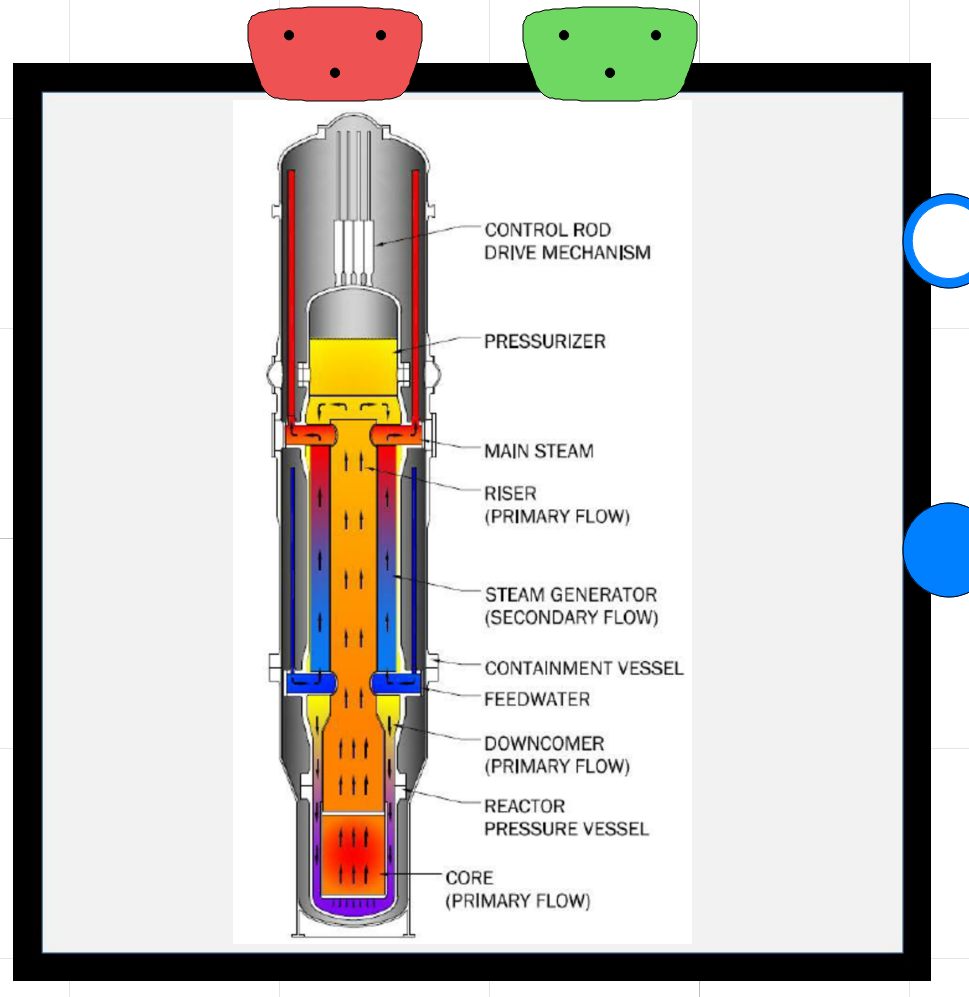
\includegraphics[scale=0.3]{pics/NuScale.png}
\caption{Top Level Depiction of the SMR System in the NHES package.}
\label{Top View NuScale Reactor}
\end{figure}

%\subsection{Cloning the Hybrid Repository}
\label{sec:clone raven}

The first step in installing the package is to clone the HYBRID repository. To do this, use
\begin{lstlisting}[language=bash]
git clone https://github.com/idaholab/HYBRID.git
\end{lstlisting}
This will download the repository into a folder called 'hybrid'. To go inside the folder, use
\begin{lstlisting}[language=bash]
cd hybrid
\end{lstlisting}


\subsubsection{Install RAVEN and its plugins as a sub-module}

The next step is to download and install RAVEN and the submodule (e.g. TEAL, HERON) plugins as a sub-module of the HYBRID repository. 

A submodule allows you to keep another Git repository in a subdirectory of your repository. The other repository has its own history, which does not interfere with the history of the current repository. This can be used to have external dependencies such as third party libraries for example.

In order to get RAVEN do the following in the hybrid folder

\begin{lstlisting}[language=bash]
git checkout devel
\end{lstlisting}

Update the Branch

\begin{lstlisting}[language=bash]
git pull
\end{lstlisting}

to add RAVEN as a submodule
\begin{lstlisting}[language=bash]
git submodule update --init --recursive
\end{lstlisting}

\textbf{Install and Compile RAVEN. }
Once you have downloaded RAVEN as a sub-module, you have to install it. go to the \href{https://github.com/idaholab/raven/wiki/intallationMain}{RAVEN Wiki} for information about how to install it. Run all the tests outlined in the RAVEN wiki. 

\subsubsection{Inform the Framework Paths}

In order to set up the hybrid repository, you must inform the framework about the location of the Dymola python interface. For doing so, navigate to the hybrid directory:

to add RAVEN as a submodule
\begin{lstlisting}[language=bash]
cd <path to your hybrid repository>/hybrid
\end{lstlisting}
Run the following command:
\begin{lstlisting}[language=bash]
./scripts/write_hybridrc.py -p DYMOLA_PATH
\end{lstlisting}

Where DYMOLAPATH is the path to the python interface egg folder in the DYMOLA installation locally. For example:
 
\begin{lstlisting}[language=bash]
./scripts/write_hybridrc.py -p 
	"/c/Program\ Files/Dymola\ 2020x/Modelica/Library/
	python_interface/dymola.egg"
\end{lstlisting}


\subsection{Energy Manifold}
The energy manifolds intention is be a diversion module to as many different subunits as needed for fluid diversion. It consists of a series of pipes that can be extended to “n” submodules, see Figure \ref{Top View Energy Manifold}. The unit has the capability of utilizing control schemes, however in many practical applications the control schemes are encapsulated within the subprocesses as opposed to within the energy manifold. There are currently four potential energy manifolds that can be used. For practical purposes only the model SteamManifold\textunderscore L1\textunderscore boundaries is used in integrated energy systems as it does not include control valves and supports “n” submodules going in and out. The other versions of the energy manifold exist for advanced users in the event the balance of plant or subprocess they are connecting to does not include sufficient valving and control to properly constrain the system. For example, simplified balance of plant systems that do not contain return flow would require the energy manifold to provide makeup water from the condenser, therefore for that scenario we would need to use the SteamManifold\textunderscore L1\textunderscore FWH\textunderscore Cond model which contains a condenser and feedwater heater.   

\begin{figure}[hbtp]
\centering
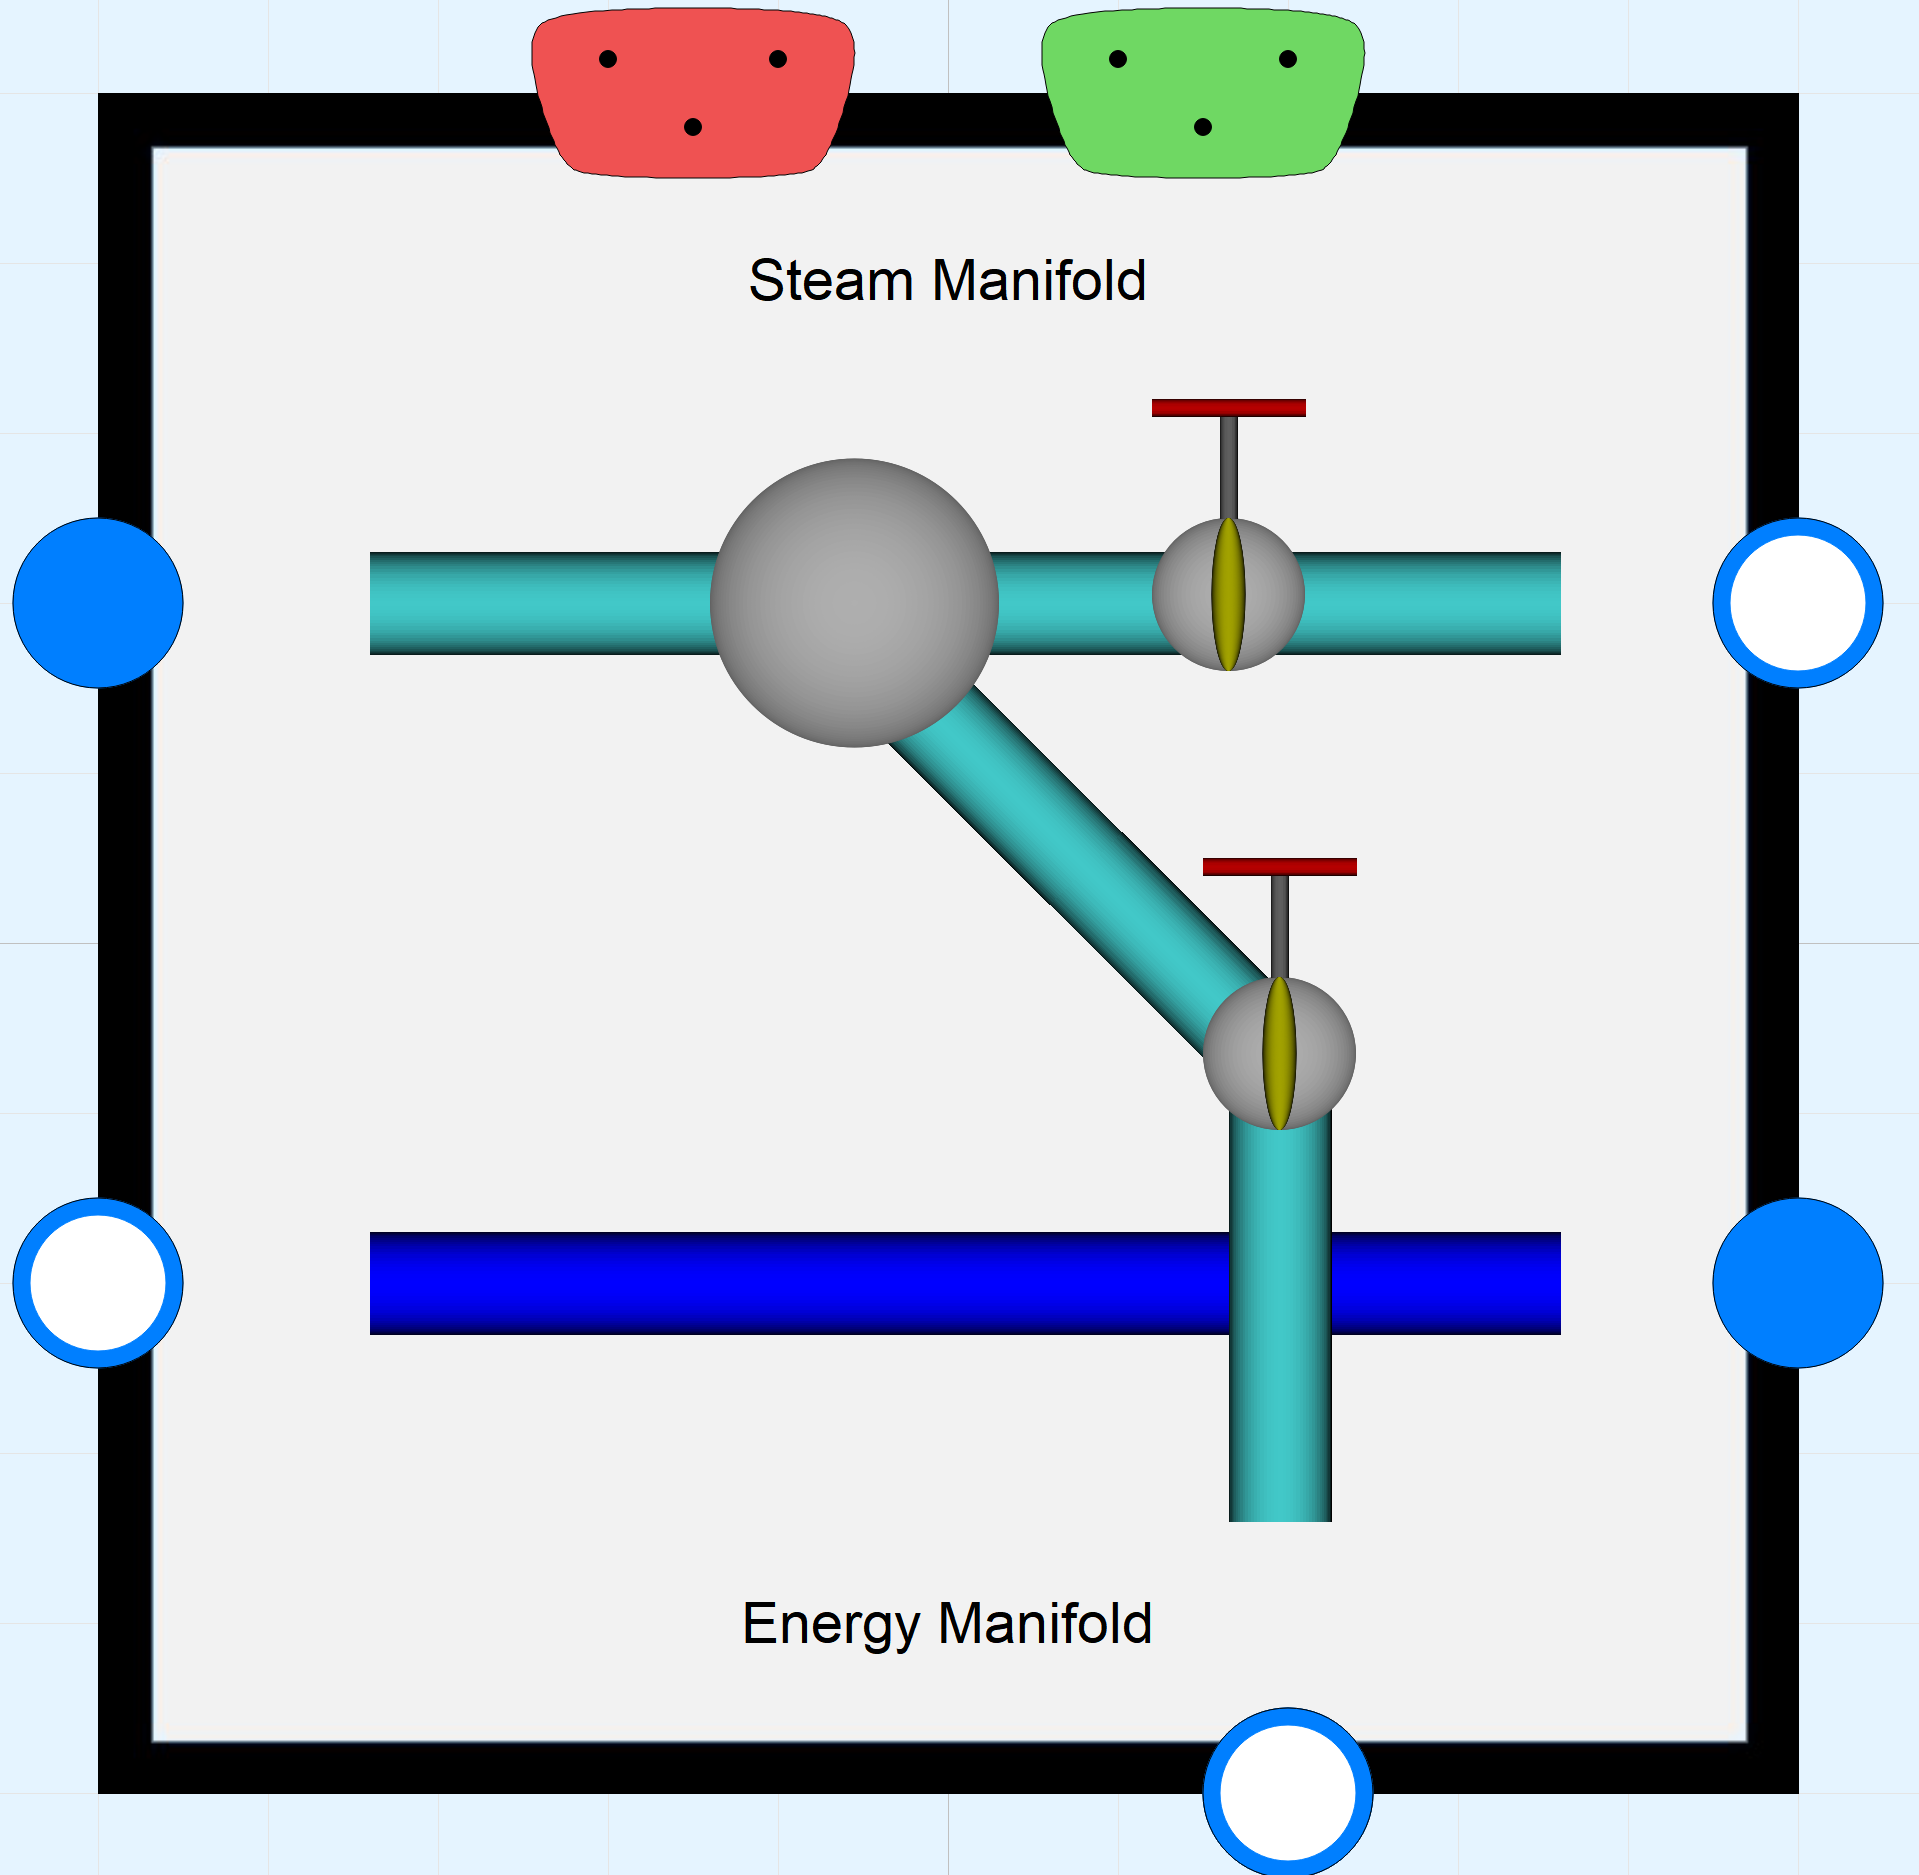
\includegraphics[scale=0.15]{pics/Energy_Manifold.png}
\caption{: Top Level Depiction of the Energy Manifold in the NHES package}
\label{Top View Energy Manifold}
\end{figure}



% content


%\subsection{Cloning the Hybrid Repository}
\label{sec:clone raven}

The first step in installing the package is to clone the HYBRID repository. To do this, use
\begin{lstlisting}[language=bash]
git clone https://github.com/idaholab/HYBRID.git
\end{lstlisting}
This will download the repository into a folder called 'hybrid'. To go inside the folder, use
\begin{lstlisting}[language=bash]
cd hybrid
\end{lstlisting}


\subsubsection{Install RAVEN and its plugins as a sub-module}

The next step is to download and install RAVEN and the submodule (e.g. TEAL, HERON) plugins as a sub-module of the HYBRID repository. 

A submodule allows you to keep another Git repository in a subdirectory of your repository. The other repository has its own history, which does not interfere with the history of the current repository. This can be used to have external dependencies such as third party libraries for example.

In order to get RAVEN do the following in the hybrid folder

\begin{lstlisting}[language=bash]
git checkout devel
\end{lstlisting}

Update the Branch

\begin{lstlisting}[language=bash]
git pull
\end{lstlisting}

to add RAVEN as a submodule
\begin{lstlisting}[language=bash]
git submodule update --init --recursive
\end{lstlisting}

\textbf{Install and Compile RAVEN. }
Once you have downloaded RAVEN as a sub-module, you have to install it. go to the \href{https://github.com/idaholab/raven/wiki/intallationMain}{RAVEN Wiki} for information about how to install it. Run all the tests outlined in the RAVEN wiki. 

\subsubsection{Inform the Framework Paths}

In order to set up the hybrid repository, you must inform the framework about the location of the Dymola python interface. For doing so, navigate to the hybrid directory:

to add RAVEN as a submodule
\begin{lstlisting}[language=bash]
cd <path to your hybrid repository>/hybrid
\end{lstlisting}
Run the following command:
\begin{lstlisting}[language=bash]
./scripts/write_hybridrc.py -p DYMOLA_PATH
\end{lstlisting}

Where DYMOLAPATH is the path to the python interface egg folder in the DYMOLA installation locally. For example:
 
\begin{lstlisting}[language=bash]
./scripts/write_hybridrc.py -p 
	"/c/Program\ Files/Dymola\ 2020x/Modelica/Library/
	python_interface/dymola.egg"
\end{lstlisting}


\subsection{Industrial Process}
Integrated Energy Systems often include thermal and electrical energy users aside the electric grid. To accommodate thermal energy users and byproduct production the HYBRID repository includes a hydrogen production unit and a reverse osmosis unit. 

\subsubsection{Hydrogen Production}
The hybrid repository includes hydrogen production via high temperature steam electrolysis (HTSE) as shown in Figure \ref{Top View HTSE}. HTSE utilizes a combination of thermal energy and electricity to split water into hydrogen (H2) and oxygen (O2) in Solid Oxide Electrolyzer Cells (SOECs), which can be seen in simple terms as the reverse operation of solid oxide fuel cells (SOFCs). The cathode-supported cell consists of a three-layer solid structure (composed of porous cathode, electrolyte, and porous anode) and an interconnect (separator) plate \cite{Udagawa}. An oxygen-ion conducting electrolyte (e.g., yttria-stabilized zirconia [YSZ] or scandia-stabilized zirconia [ScSZ]) is generally used in SOECs \cite{JimObrien}. For electrically conducting electrodes, a nickel cermet cathode, and a perovskite anode such as strontium-doped lanthanum manganite (LSM) are typically used. The interconnect plate separates the process gas streams; it must also be electrically conducting and is usually metallic, such as a ferritic stainless steel. 

For the HTSE models there are four main models developed by INL, each relying on the same underlying physics of the system but with different control schemes. The HTSE units within the Modelica framework have been specifically designed for integration with light water reactor systems and have been sized with the necessary components to allow for steam side preheating under this assumption. It should be noted that in other HTSE designs there may be varying degrees of preheating equipment based on inlet conditions from the external process. For the HTSE process system parameters are finely tuned and highly non-linear when compared with other process models. Changes in heat exchanger design and sizing can be made directly within the subsystem model however due to the nonlinearity of the system convergence following any changes, a singular component cannot be guaranteed. To modify HTSE stack characteristics the user will need to go two levels down into the HTSE stack system the HTSE stack can be clicked on to open a parameter table where stack characteristics can be modified. Due to the high level of complexity required with HTSE stacks and the customization required depending on the inlet conditions of external system usage of the existing HTSE is preferred, with more details available in two reports published. \cite{2016HTSE},\cite{2017HTSE},\cite{JongHydrogen}. Base classes for the HTSE system can found in the “Electrolysis” package within the NHES framework and can be utilized if one desires to create their own HTSE unit. 

\begin{figure}[hbtp]
\centering
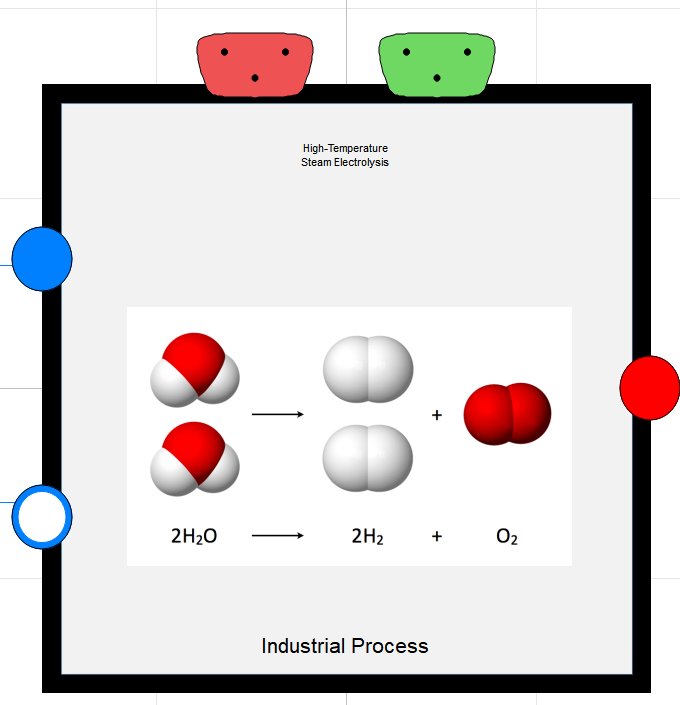
\includegraphics[scale=0.4]{pics/HTSE.png}
\caption{Top Level Depiction of the High Temperature Steam Electrolysis Unit in the NHES package}
\label{Top View HTSE}
\end{figure}



\subsubsection{Desalination}
The NHES repository includes a desalination industrial process based on reverse osmosis (RO), Figure \ref{Top View Reverse Osmosis}, designed for brackish water desalination. RO desalination utilizes a semi-permeable membrane, which allows water to pass through but not salts, thus separating the fresh water from the saline feed water. A typical Brackish Water RO (BWRO) plant consists of four main components: feed water pretreatment, High-Pressure (HP) pumping, membrane separation, and permeate (fresh water) post-treatment. The concentrate water rejected by the first membrane module plays a role as the feed water for the second membrane module by the successive order, and so on. These pressure vessels are arranged in rows in each membrane stage, with two-stage membrane separation being typical in BWRO. Each stage has a recovery of 50–60 percent, achieving overall system recovery of 70–85 percent \cite{JongDesalination}. 

The Reverse Osmosis Subsystem unit provides the user the ability to modify the number of parallel reverse osmosis units being utilized within the plant alongside to specify how much power is being input into the RO system. Each one of these parallel systems is assumed to go through a two-step the desalination process. In addition, the unit provides the user the ability to alter the salinity of the brine coming into the plant alongside a specified pressure differential across the plant. If further alterations and control are desired from a user perspective reports detailing the full specifications of the plant designs are available in \cite{2018ThermalStorage}, \cite{JongDesalination}. Additionally, base components for the entire desalination plant can be found in the “Desalination” package within the NHES repository. 
 

\begin{figure}[hbtp]
\centering
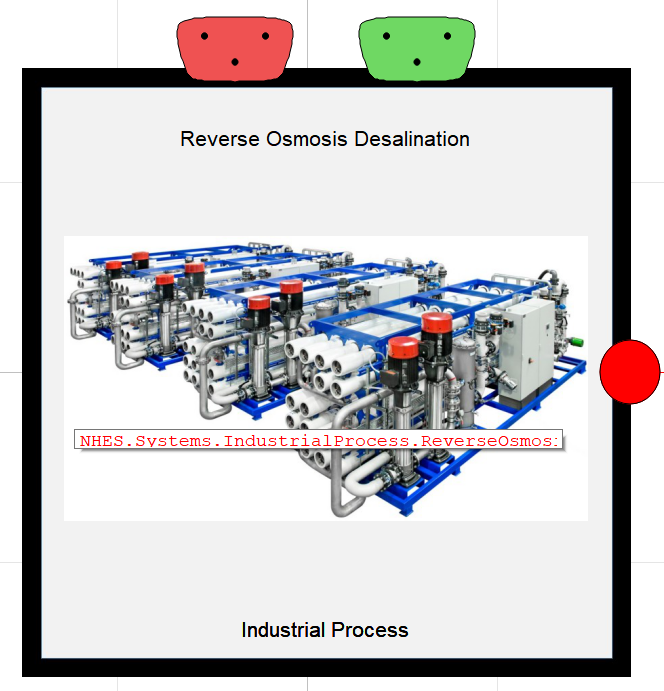
\includegraphics[scale=0.3]{pics/Desalination Plant.png}
\caption{Top Level Depiction of the Brackish Water Desalination Process in the NHES package}
\label{Top View Reverse Osmosis}
\end{figure}



% content


%\subsection{Cloning the Hybrid Repository}
\label{sec:clone raven}

The first step in installing the package is to clone the HYBRID repository. To do this, use
\begin{lstlisting}[language=bash]
git clone https://github.com/idaholab/HYBRID.git
\end{lstlisting}
This will download the repository into a folder called 'hybrid'. To go inside the folder, use
\begin{lstlisting}[language=bash]
cd hybrid
\end{lstlisting}


\subsubsection{Install RAVEN and its plugins as a sub-module}

The next step is to download and install RAVEN and the submodule (e.g. TEAL, HERON) plugins as a sub-module of the HYBRID repository. 

A submodule allows you to keep another Git repository in a subdirectory of your repository. The other repository has its own history, which does not interfere with the history of the current repository. This can be used to have external dependencies such as third party libraries for example.

In order to get RAVEN do the following in the hybrid folder

\begin{lstlisting}[language=bash]
git checkout devel
\end{lstlisting}

Update the Branch

\begin{lstlisting}[language=bash]
git pull
\end{lstlisting}

to add RAVEN as a submodule
\begin{lstlisting}[language=bash]
git submodule update --init --recursive
\end{lstlisting}

\textbf{Install and Compile RAVEN. }
Once you have downloaded RAVEN as a sub-module, you have to install it. go to the \href{https://github.com/idaholab/raven/wiki/intallationMain}{RAVEN Wiki} for information about how to install it. Run all the tests outlined in the RAVEN wiki. 

\subsubsection{Inform the Framework Paths}

In order to set up the hybrid repository, you must inform the framework about the location of the Dymola python interface. For doing so, navigate to the hybrid directory:

to add RAVEN as a submodule
\begin{lstlisting}[language=bash]
cd <path to your hybrid repository>/hybrid
\end{lstlisting}
Run the following command:
\begin{lstlisting}[language=bash]
./scripts/write_hybridrc.py -p DYMOLA_PATH
\end{lstlisting}

Where DYMOLAPATH is the path to the python interface egg folder in the DYMOLA installation locally. For example:
 
\begin{lstlisting}[language=bash]
./scripts/write_hybridrc.py -p 
	"/c/Program\ Files/Dymola\ 2020x/Modelica/Library/
	python_interface/dymola.egg"
\end{lstlisting}


\subsection{Balance of Plant}
There are two main balance of plant models in the hybrid repository. The standard ideal turbine (with and without a condenser and feedwater heater) and step down turbines that allow turbine tap offtake.


\subsubsection{Simple Balance of Plant}

The balance of plant system consists of an ideal steam turbine model, a condenser, feedwater system for reheat, and a couple of valves that allow steam flow either to the turbine or as bypass to the condenser, Figure \ref{Top View SimpleBOP}. Additionally, piping exists to send condensate and rejected heat from ancillary processes directly to the condenser. The balance of plant model can handle supervisory control input for direct control of the turbine control valve and turbine bypass valve based on different sensor input. The main balance of plant system is designed to model Rankine systems.  

\begin{figure}[hbtp]
\centering
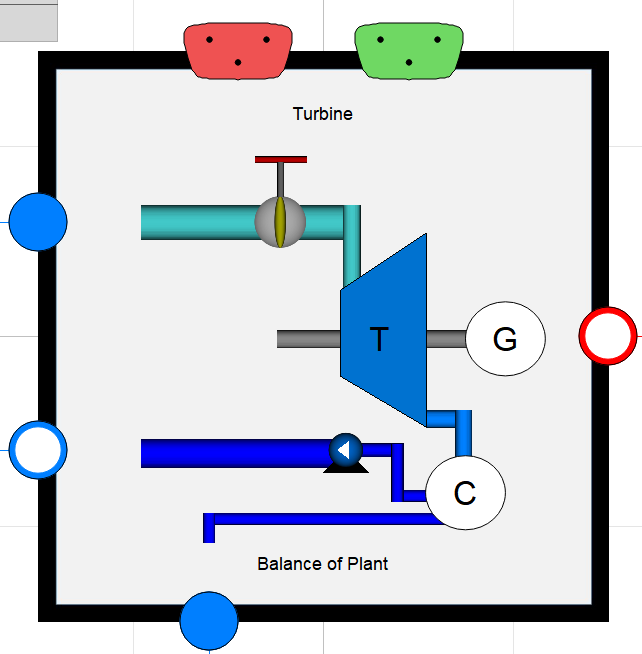
\includegraphics[scale=0.4]{pics/BOP.png}
\caption{Top Level Depiction of the Balance of Plant in the NHES package}
\label{Top View SimpleBOP}
\end{figure}


\subsubsection{Step Down Turbines}

The step-down turbines consist of a series of an ideal steam turbines connected via a singular rotational inertia shaft with bypass tap lines coming off the turbines, Figure \ref{Top View Step Down Turbines}. The purpose of this model is to allow turbine tap offtake in a dynamic system. The data record within the model includes a series of inputs that allows the user to specify the turbine tap offtake pressures. Additionally, each individual offtake fraction can be input from the data record. The outlet of the stepdown turbines does not include a condenser; therefore, a condenser model would need to be included in a separate system model if the fluid is to be re-introduced into an overall system model.
 
\begin{figure}[hbtp]
\centering
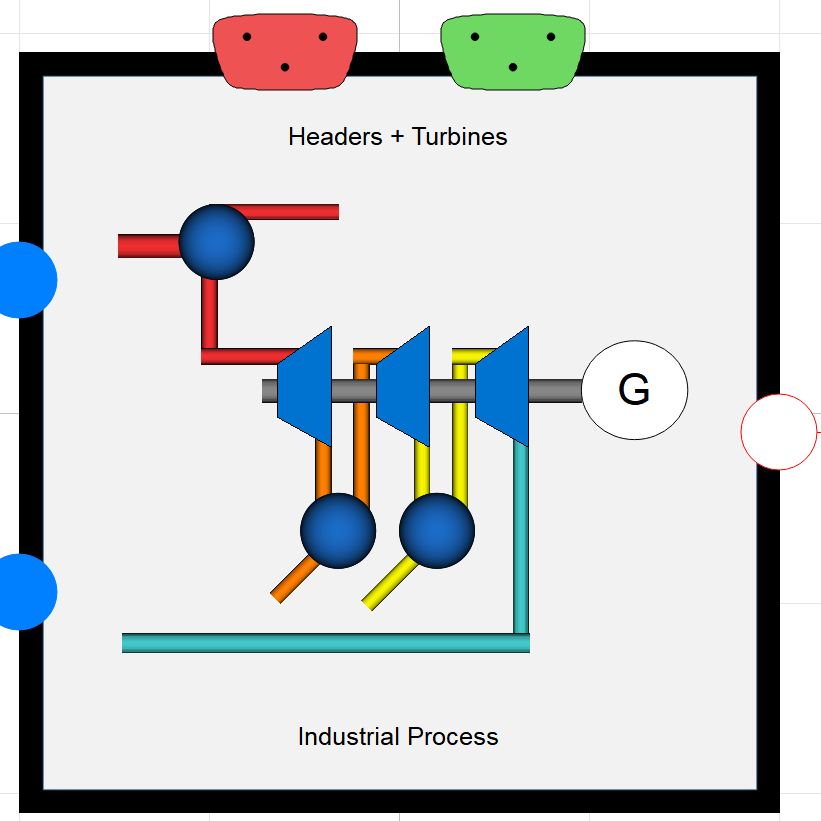
\includegraphics[scale=0.3]{pics/HeaderStepdownturbines.png}
\caption{Top Level Depiction of the StepDown Turbines in the NHES package}
\label{Top View Step Down Turbines}
\end{figure}


\subsubsection{Stage by Stage Turbine}
The stage by stage turbine package is designed to allow for detailed design of a Rankine cycle: including all turbine taps, moisture separators, reheaters, fluid junctions, and peaking capabilities. The model uses geometric design rather than system design (pressure ratios, setpoints, efficiencies). The primary design values are cross sectional and design flow deflection angles. Pressure, mass flow rate, and entropic efficiency are all uncontrolled and unspecified. 


\begin{figure}[hbtp]
\centering
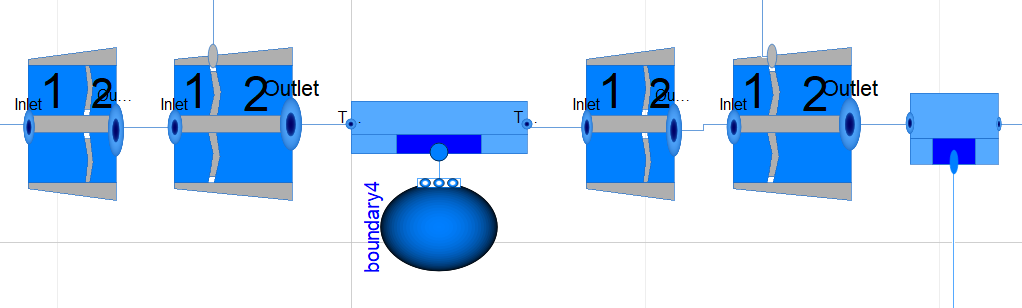
\includegraphics[scale=0.75]{pics/StagebyStageTurbine.png}
\caption{Top Level Stage by Stage Turbine Section With Stators, Rotors, a Tap, and a Moisture Separator}
\label{TVSbST}
\end{figure}


There are 8 primary components used to develop a full stage by stage turbine system. Multiple are shown in Figure \ref{TVSbST}. The first are the turbine inlet and turbine outlet components which allow for transition between 1D axial fluid components and 3D velocity cylindrical fluid flow components. The next components are the stator and rotor stages. Stator stages deflect incoming flow to better impinge and deposit energy on rotating rotor stages. Rotor stages additionally have torque connectors to connect to a physical turbine model which is responsible for linking the rotor stage torque to the electrical generator. T-junction components setup for cylindrical flow connectors allow for overpowering a rated turbine flow. The final two components deal with removing flow from the turbine. One is a turbine tap, which sets pressures equal between stages. The other is a moisture separator that removes a specific fraction of liquid flow quality. 

The stage by stage turbine has been tested from 50-100 percent steam flow. 


% content


%\subsection{Cloning the Hybrid Repository}
\label{sec:clone raven}

The first step in installing the package is to clone the HYBRID repository. To do this, use
\begin{lstlisting}[language=bash]
git clone https://github.com/idaholab/HYBRID.git
\end{lstlisting}
This will download the repository into a folder called 'hybrid'. To go inside the folder, use
\begin{lstlisting}[language=bash]
cd hybrid
\end{lstlisting}


\subsubsection{Install RAVEN and its plugins as a sub-module}

The next step is to download and install RAVEN and the submodule (e.g. TEAL, HERON) plugins as a sub-module of the HYBRID repository. 

A submodule allows you to keep another Git repository in a subdirectory of your repository. The other repository has its own history, which does not interfere with the history of the current repository. This can be used to have external dependencies such as third party libraries for example.

In order to get RAVEN do the following in the hybrid folder

\begin{lstlisting}[language=bash]
git checkout devel
\end{lstlisting}

Update the Branch

\begin{lstlisting}[language=bash]
git pull
\end{lstlisting}

to add RAVEN as a submodule
\begin{lstlisting}[language=bash]
git submodule update --init --recursive
\end{lstlisting}

\textbf{Install and Compile RAVEN. }
Once you have downloaded RAVEN as a sub-module, you have to install it. go to the \href{https://github.com/idaholab/raven/wiki/intallationMain}{RAVEN Wiki} for information about how to install it. Run all the tests outlined in the RAVEN wiki. 

\subsubsection{Inform the Framework Paths}

In order to set up the hybrid repository, you must inform the framework about the location of the Dymola python interface. For doing so, navigate to the hybrid directory:

to add RAVEN as a submodule
\begin{lstlisting}[language=bash]
cd <path to your hybrid repository>/hybrid
\end{lstlisting}
Run the following command:
\begin{lstlisting}[language=bash]
./scripts/write_hybridrc.py -p DYMOLA_PATH
\end{lstlisting}

Where DYMOLAPATH is the path to the python interface egg folder in the DYMOLA installation locally. For example:
 
\begin{lstlisting}[language=bash]
./scripts/write_hybridrc.py -p 
	"/c/Program\ Files/Dymola\ 2020x/Modelica/Library/
	python_interface/dymola.egg"
\end{lstlisting}


\subsection{Energy Storage}
Energy Storage is a large component of Integrated Energy Systems. Currently there are two models of Energy Storage in the repository. Electric Battery Storage, characterized largely as Li-ion battery technology, and two-tank sensible heat thermal energy storage that uses Therminol-66 as the working fluid. 


\subsubsection{Electric Battery Storage}

Electric Battery Storage, shown in Figure \ref{Top View Logical Battery}, is largely characterized as fast and expensive. Due to the speed with which battery storage systems operate, on the order milliseconds, the battery within the hybrid repository has been modeled as a simple logical battery system. The battery can both charge and discharge based upon the direction of electricity flow through the port. It is assumed to be a “perfect” battery and due to the speed of the system, subcomponents have not been modeled simply because they would operate faster than would be useful for the types of analysis utilized with the system. The battery has user-based inputs that control how fast or slow the system can charge and discharge as well as how much energy can be stored within the battery before it is considered full.   

\begin{figure}[hbtp]
\centering
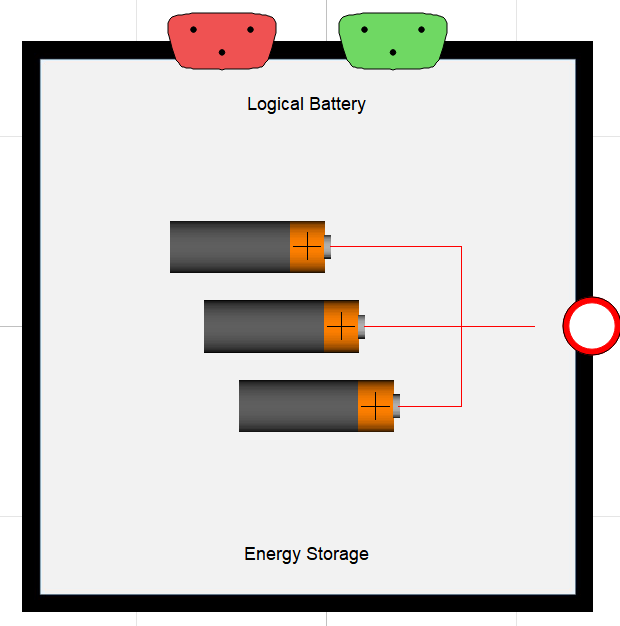
\includegraphics[scale=0.4]{pics/Battery_Storage.png}
\caption{Top Level Depiction of the Logical Battery in the NHES package}
\label{Top View Logical Battery}
\end{figure}


\subsubsection{Two-Tank Thermal Energy Storage}

Sensible heat storage involves the heating of a solid or liquid without phase change and can be deconstructed into two operating modes: charging and discharging. A two-tank TES system, shown in Figure \ref{Top View Two Tank Sensible Storage}, is a common configuration for liquid sensible heat systems. In the charging mode cold fluid is pumped from a cold tank through an Intermediate Heat Exchanger (IHX), heated, and stored in a hot tank while the opposite occurs in the discharge mode. Such systems have been successfully demonstrated in the solar energy field as a load management strategy. The configuration of the TES system held within the repository involves an outer loop interfaces with the energy manifold. Bypass steam is directed through an IHX and ultimately discharged to the main condenser of an Integrated system. An inner loop containing a TES fluid consists of two large storage tanks along with several pumps to transport the TES fluid between the tanks, the IHX and a steam generator. Flow Bypass Valves (FBVs) are included in the discharge lines of both the “hot” and “cold” tanks to prevent deadheading the pumps when the Flow Control Valves (FCVs) are closed. Therminol-66 is chosen as the TES fluid as it is readily available, can be pumped at low temperatures, and offers thermal stability over the range (-3°C–343°C) which covers the anticipated operating range of the light water reactor systems (203°C–260°C). Molten salts (e.g. 48 percent  NaNO3 – 52 percent KNO3) were not considered, as the anticipated operating temperatures fall below their 222°C freezing temperature. The TES system is designed to allow the power plant to run continuously at ~100 percent power over a wide range of operating conditions. During periods of excess capacity, bypass steam is directed to the TES unit through the auxiliary bypass valves where it condenses on the shell side of the IHX. TES fluid is pumped from the cold tank to the hot tank through the tube side of the IHX at a rate sufficient to raise the temperature of the TES fluid to some set point. The TES fluid is then stored in the hot tank at constant temperature. Condensate is collected in a hot well below the IHX and drains back to the main condenser or can be used for some other low pressure application such as chilled water production, desalination or feed-water heating. The system is discharged during periods of peak demand, or when process steam is desired, by pumping the TES fluid from the hot tank through a boiler (steam generator) to the cold tank. This process steam can then be reintroduced into the power conversion cycle for electricity production or directed to some other application through the PCV. A nitrogen cover gas dictates the tank pressures during charging and discharging operation. Full details of the model and its use within integrated energy systems can be found in report \cite{2018ThermalStorage}, \cite{FrickThermalStorage}. 

The model itself is coded in a non-conventional manner compared to the rest of the modelica models. It is coded in an input, output sense rather than in a fluid-port, electric-port based modeling system. This is because the model was transferred over from a FORTRAN style code rather than initially coded in Modelica. To modify the two-tank thermal storage system the user will need to look at each individual model within the charging mode and the discharge mode. Base components within the models are fully commented within the code. Like the HTSE the thermal storage unit is finely tuned and thus use outside of its current state will take a bit of work. To help with this the thermal storage unit has been sized to be compatible for varying sizes of offtake from a power unit. One is sized to take 20 percent of nominal steam from a standard 3400MWt Westinghouse plant, and one is designed for 5 percent offtake. Both designed to provide energy back as a peaking unit. The peaking unit is held within the discharge side of the model and is assumed to have its own turbine or is sent back to the low-pressure turbine. Explicit modeling of the coupling back with the low-pressure turbine has not been done. Future updating of the two-tank thermal storage unit to be consistent with other models is planned.

 
\begin{figure}[hbtp]
\centering
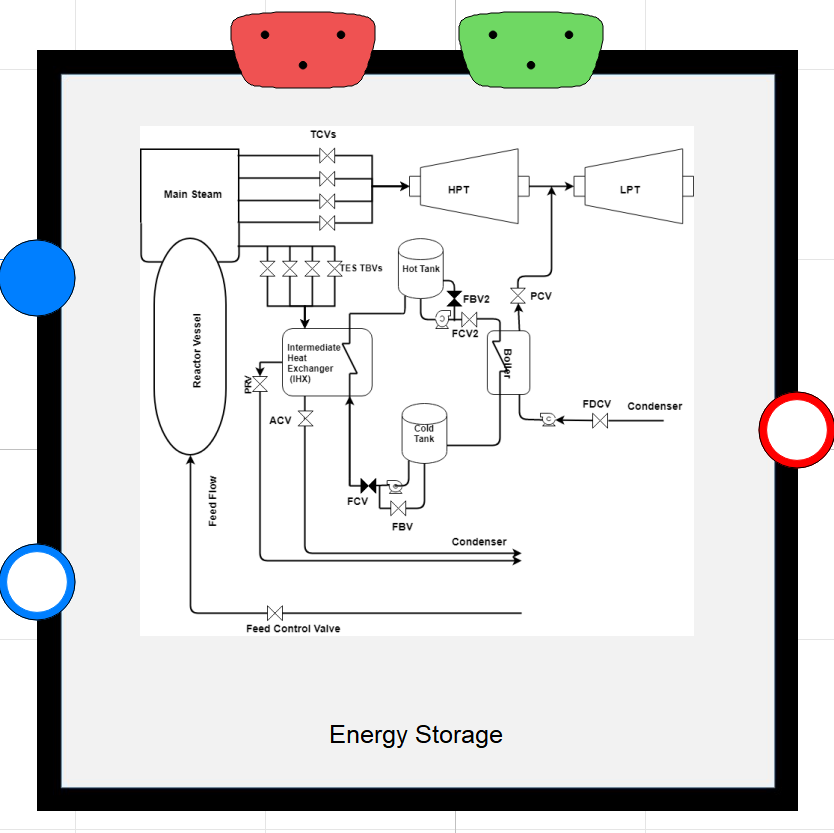
\includegraphics[scale=0.3]{pics/Sensible_Heat_System.png}
\caption{Top Level Depiction of the Two-Tank Sensible Heat Storage Unit in the NHES package}
\label{Top View Two Tank Sensible Storage}
\end{figure}

% content
\subsubsection{Thermocline Packed Bed Thermal Energy Storage}
A thermocline storage system, shown in Figure \ref{Top View Thermocline}, stores heat via hot and cold fluid separated by a thin thermocline region that arises due to density differential between the fluid. Assuming low mixing via internal flow characteristics and structural design, this thermocline region can be kept relatively small in comparison with the size of the tank. Additionally, large buoyancy changes and low internal thermal conductivity are also extremely useful in maintaining small relative thermocline thickness.

To increase the cost-effective nature of these designs, it is common to fill the tank with a low-cost filler material, such as concrete or quartzite. These filler materials are cheap, have high density, and high thermal conductivity. By using such material, a reduction in the amount of high cost thermal fluid can be achieved, thereby increasing the economic competitiveness of such designs.

The thermocline system was modeled from a modified set of Schumann equations that were originally introduced in 1927 \cite{Schumann}. The equation set governs energy conservation of fluid flow through porous media. His equation set has been widely adopted in the analysis of thermocline storage tanks. The modified equations adopted a new version of the convective heat-transfer coefficient to incorporate low and no-flow conditions from Gunn in 1978 \cite{specialHeattransfer}. Additionally, a conductive heat-transfer term was added for the heat conduction through the walls of the tank. Self-degradation of the thermocline in the axial direction is neglected due to low relative values when during standard operation, this is a known limit of the model during times of no flow.

\begin{figure}[hbtp]
\centering
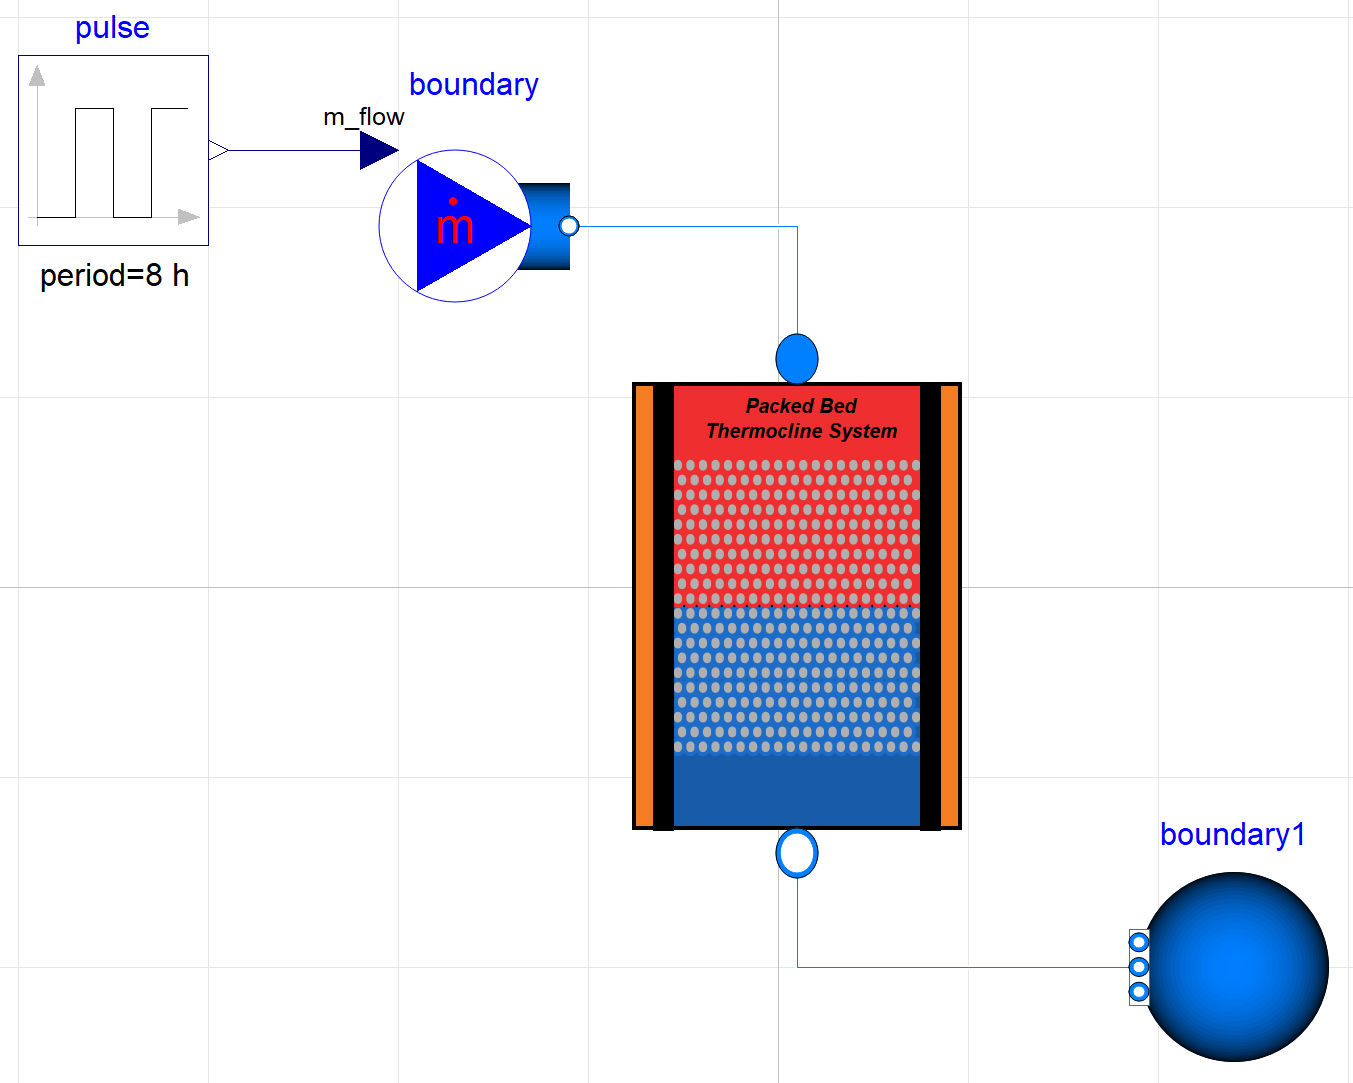
\includegraphics[scale=0.3]{pics/Thermocline_Test.png}
\caption{Top Level Depiction of the Single Tank Packed Bed Heat Storage Unit in the NHES package}
\label{Top View Thermocline}
\end{figure}

\subsubsection{Concrete Solid Media Storage}

Three different models exist for concrete solid media storage, shown in Figure \ref{CTES}. Concrete solid media storage uses inexpensive materials to charge and discharge heat from a fluid system. The models within the Hybrid system use HeatCrete as the concrete material, the properties of which are found in literature. The initial development has been done with energy arbitrage for a Rankine system in mind. However, there are not limitations on the heat transfer fluid that can be used in conjunction with the concrete system. Two design modalities exist with the three developed models. One is a single pipe model and the other is a dual pipe model. All models use simplified flow models: a single pressure and mass flow rate is imposed within a pipe (which allows for significantly improved performance at low and no flow rate conditions) leaving the dynamics of the system to primarily be described by the conservation of energy equation. Within the concrete model, heat conducts both radially and axially in a 2-D nodalized vector. All models calculate values for an average pipe and the system behavior is then scaled by the number of pipes. 

The single pipe model is so called because it only models one fluid pipe within a concrete system. This modeling choice imposes a restriction that heat transfer fluid only flows in one direction or the other (note, no error signals are sent by this, m\textunderscore flow\textunderscore internal = m\textunderscore flow\textunderscore ch-m\textunderscore flow\textunderscore dis). The behavior of this system lends itself better to batch energy applications. The power level during quenching (HTF quenching during charging or concrete quenching during discharging) is an order of magnitude higher than the steady power level. The pressure of the system is taken at the cold end, and defaults to the charging pressure. This model can operate in charging, discharging, OR standby mode. The single pipe model operates with an established axial thermocline and a reversing radial thermal gradient depending on operation. 

The dual pipe and dual pipe two HTFs model contain separate pipes for the charging and discharging flow. This model operates more steadily over long periods of time. Heat is always conducted within the CTES and between the concrete and the HTFs. The dual pipe CTES can operate in charging, discharging, standby, or thermal buffer (both charging and discharging) modes. The dual pipe system operates with mono-directional thermal gradients in both axial and radial directions in all operating modes. 


\begin{figure}[hbtp]
\centering
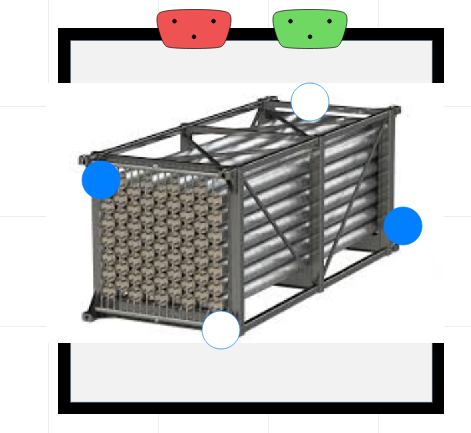
\includegraphics[scale=0.8]{pics/CTES.png}
\caption{Top Level Depiction of Concrete Thermal Energy Storage System}
\label{CTES}
\end{figure}

%\subsection{Cloning the Hybrid Repository}
\label{sec:clone raven}

The first step in installing the package is to clone the HYBRID repository. To do this, use
\begin{lstlisting}[language=bash]
git clone https://github.com/idaholab/HYBRID.git
\end{lstlisting}
This will download the repository into a folder called 'hybrid'. To go inside the folder, use
\begin{lstlisting}[language=bash]
cd hybrid
\end{lstlisting}


\subsubsection{Install RAVEN and its plugins as a sub-module}

The next step is to download and install RAVEN and the submodule (e.g. TEAL, HERON) plugins as a sub-module of the HYBRID repository. 

A submodule allows you to keep another Git repository in a subdirectory of your repository. The other repository has its own history, which does not interfere with the history of the current repository. This can be used to have external dependencies such as third party libraries for example.

In order to get RAVEN do the following in the hybrid folder

\begin{lstlisting}[language=bash]
git checkout devel
\end{lstlisting}

Update the Branch

\begin{lstlisting}[language=bash]
git pull
\end{lstlisting}

to add RAVEN as a submodule
\begin{lstlisting}[language=bash]
git submodule update --init --recursive
\end{lstlisting}

\textbf{Install and Compile RAVEN. }
Once you have downloaded RAVEN as a sub-module, you have to install it. go to the \href{https://github.com/idaholab/raven/wiki/intallationMain}{RAVEN Wiki} for information about how to install it. Run all the tests outlined in the RAVEN wiki. 

\subsubsection{Inform the Framework Paths}

In order to set up the hybrid repository, you must inform the framework about the location of the Dymola python interface. For doing so, navigate to the hybrid directory:

to add RAVEN as a submodule
\begin{lstlisting}[language=bash]
cd <path to your hybrid repository>/hybrid
\end{lstlisting}
Run the following command:
\begin{lstlisting}[language=bash]
./scripts/write_hybridrc.py -p DYMOLA_PATH
\end{lstlisting}

Where DYMOLAPATH is the path to the python interface egg folder in the DYMOLA installation locally. For example:
 
\begin{lstlisting}[language=bash]
./scripts/write_hybridrc.py -p 
	"/c/Program\ Files/Dymola\ 2020x/Modelica/Library/
	python_interface/dymola.egg"
\end{lstlisting}


\subsubsection{Latent Heat Thermal Energy Storage}

Latent heat energy storage stores energy in materials undergoing phase change. These phase change materials (PCMs) can undergo melting and fusion, boiling and condensation, or hydration and dehydration. PCMs have high volumetric and mass-specific energy storage densities. They can theoretically operate isothermally as the phase change occurs at a single temperature. The ideal PCM would have a large latent heat associated with its phase change, little to no density change between phases, indefinite cyclability between phases, and high thermal conductivity. Research continues in PCMs to identify enhancements that would allow lab-scale experiments to increase size to demonstrate grid-scale applications. A significant challenge is enhancing the thermal conductivity in the PCMs. As the charging or discharging HTF will drive the phase change condition at the heat transfer surface, continuing that process into the PCM mass is based on the thermal conductivity of the material. Conductivity enhancement via geometry specification, micro-encapsulation, and material impregnation has been investigated over time. 

The most common PCMs identified operate between the solid and liquid phases where the density change is minimal. Because the melting or solidification front is key to moving heat between the HTF and the PCMs, many high-fidelity models have been developed across the research field. The model available in the HYBRID repository is based on a paraffin wax experiment. The experiment used water as the HTF to melt and solidify paraffin wax. The original model was built in Star-CCM+ and then converted to Matlab. The Matlab version subsequently has been converted into a Modelica model within HYBRID. The generalized low-fidelity model has been built to accommodate new geometric designs, materials, and HTFs. 


The model is a two-dimensional radial conductivity model across three materials: the HTF, a pipe wall, then through the PCM as shown in Figure \ref{PCM}. Within the fluid, the following equation set applies. The equations are also applied within the tube, but the velocity term disappears without internal mass movement. The term $\alpha$ is thermal resistance, equal to thermal conductivity divided by the density and specific heat capacity. 


\[\frac{dT}{dt} = \alpha\nabla^{2}T - (\overrightarrow{v}\cdot\nabla T)\]

Effectively, the equation set is applied across the material interfaces, with an effective interface thermal conductivity

\[k_{eff}=\frac{2k_{1}k_{2}}{k_{1}+k_{2}}\]

Because there is phase change within the PCM. The equation is written in terms of enthalpy instead of temperature, and the PCM temperature is calculated as a function of the enthalpy (h). 

\[\frac{dh}{dt} = \alpha\nabla^{2}h\]

\begin{figure}[hbtp]
\centering
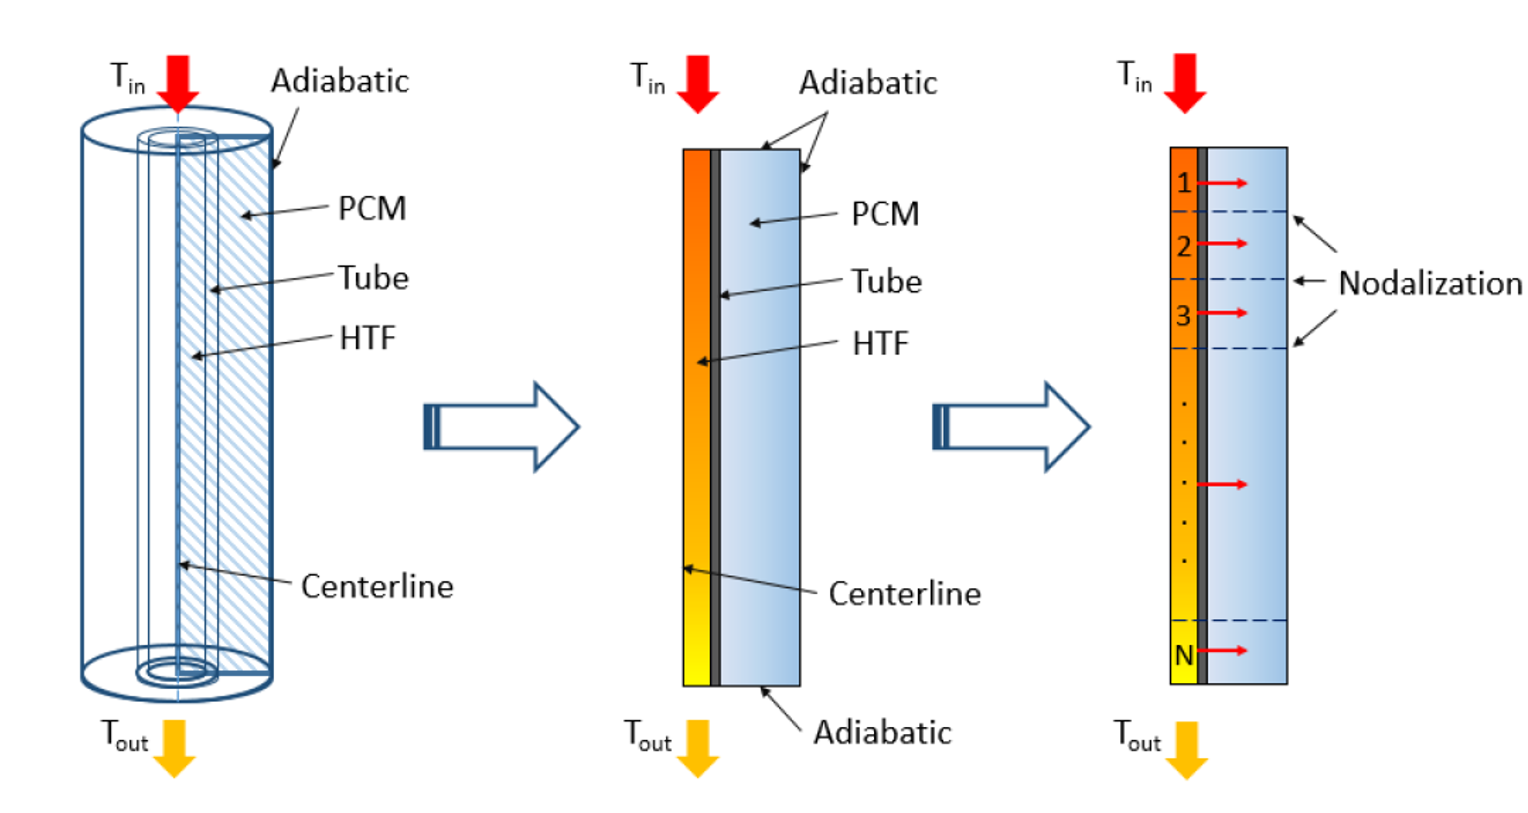
\includegraphics[scale=0.5]{pics/PCM.png}
\caption{PCM Nodalization diagram}
\label{PCM}
\end{figure}

The initial models built in Matlab and Star-CCM+ used constant fluid properties and an assumed inlet velocity. The Modelica model has a fluid inlet and exit to allow for replacement of the HTF in the model, and for outer conditions to dictate to the PCM model the fluid conditions at the interfaces. 





\subsection{Secondary Energy Source}
Secondary Energy Sources, or commonly known as peaking units, are an essential part of the energy grid. These systems provide "on-demand" energy during moments when the electrical demand is larger than what the rest of the grid can accomodate. A common feature of 

\subsubsection{Natural Gas Fired Turbine}

Recently, natural gas-fired turbines have found widespread use because of their higher efficiencies, lower capital costs, shorter installation times, abundance of natural gas supplies, lower greenhouse gas emissions compared to other energy sources; and fast start-up capability, which enables them to be used as peaking units that respond to peak demands \cite{GasTurbine2008}, \cite{GasTurbine2013}. Due to their special characteristics, natural gas fired turbines are installed in numerous places around the world and have become an important source for power generation. This section is dedicated to detailed process and control designs of the GTPP, whose primary role is to cover rapid dynamics in grid demand that cannot be met by the remainder of the N-R HES. Simulation results involving several case studies are also provided. Full system details are available in OSTI \cite{2016HTSE}.

The natural gas turbine, Figure \ref{Top View Gas Turbine}, is designed with parameters embedded in each individual component. The top level variables can be edited directly within the GTTP\textunderscore PowerCtrl system. This component is where things such as pressure ratios, flow rates, mechanical efficiencies, and shaft inertia can be modified. The natural gas turbine is designed with a nominal electrical power generation capacity of 35MWe but has a specially designed capacityScaler variable that allows the user to scale the system to between 17 and 70MWe for a singular load. If more are desired then the deployment of several natural gas fired turbines would be required. 

\begin{figure}[hbtp]
\centering
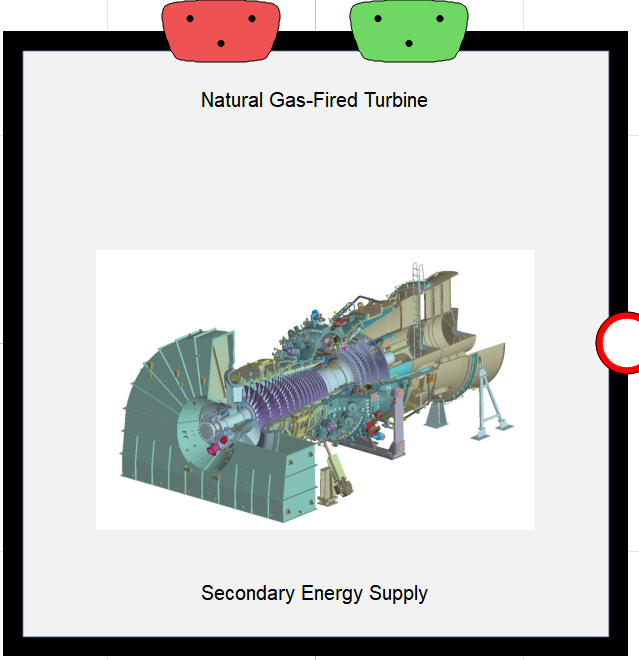
\includegraphics[scale=0.4]{pics/GasTurbine.png}
\caption{Top Level Depiction of the Natural Gas Fired Turbine in the NHES package}
\label{Top View Gas Turbine}
\end{figure}

\subsubsection{Hydrogen Turbine}
With the increase in hydrogen production technologies comes on the other end hydrogen burning technologies. To accommodate a hydrogen burning technology the HYBRID repository has been outfitted with a retrofit natural gas burner that is capable of handling pure hydrogen. 

The hydrogen turbine, Figure \ref{Top View Hydrogen Turbine}, is designed with parameters embedded in each individual component. The top level variables can be edited directly within the Hydrogen\textunderscore PowerCtrl system. This component is where things such as pressure ratios, flow rates, mechanical efficiencies, and shaft inertia can be modified. The hydrogen turbine is designed with a nominal electrical power generation capacity of 35MWe but has a specially designed capacityScaler variable that allows the user to scale the system to between 17 and 70MWe for a singular load. If more are desired then the deployment of several hydrogen turbines would be required. 


\begin{figure}[hbtp]
\centering
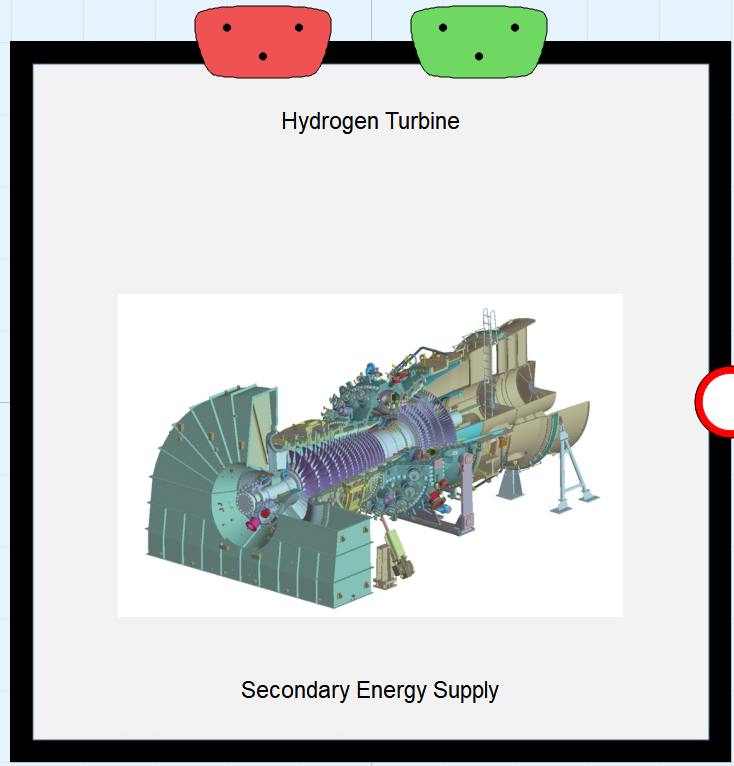
\includegraphics[scale=0.4]{pics/Hydrogen_Turbine.png}
\caption{Top Level Depiction of the Hydrogen Turbine in the NHES package}
\label{Top View Hydrogen Turbine}
\end{figure}
%\subsection{Cloning the Hybrid Repository}
\label{sec:clone raven}

The first step in installing the package is to clone the HYBRID repository. To do this, use
\begin{lstlisting}[language=bash]
git clone https://github.com/idaholab/HYBRID.git
\end{lstlisting}
This will download the repository into a folder called 'hybrid'. To go inside the folder, use
\begin{lstlisting}[language=bash]
cd hybrid
\end{lstlisting}


\subsubsection{Install RAVEN and its plugins as a sub-module}

The next step is to download and install RAVEN and the submodule (e.g. TEAL, HERON) plugins as a sub-module of the HYBRID repository. 

A submodule allows you to keep another Git repository in a subdirectory of your repository. The other repository has its own history, which does not interfere with the history of the current repository. This can be used to have external dependencies such as third party libraries for example.

In order to get RAVEN do the following in the hybrid folder

\begin{lstlisting}[language=bash]
git checkout devel
\end{lstlisting}

Update the Branch

\begin{lstlisting}[language=bash]
git pull
\end{lstlisting}

to add RAVEN as a submodule
\begin{lstlisting}[language=bash]
git submodule update --init --recursive
\end{lstlisting}

\textbf{Install and Compile RAVEN. }
Once you have downloaded RAVEN as a sub-module, you have to install it. go to the \href{https://github.com/idaholab/raven/wiki/intallationMain}{RAVEN Wiki} for information about how to install it. Run all the tests outlined in the RAVEN wiki. 

\subsubsection{Inform the Framework Paths}

In order to set up the hybrid repository, you must inform the framework about the location of the Dymola python interface. For doing so, navigate to the hybrid directory:

to add RAVEN as a submodule
\begin{lstlisting}[language=bash]
cd <path to your hybrid repository>/hybrid
\end{lstlisting}
Run the following command:
\begin{lstlisting}[language=bash]
./scripts/write_hybridrc.py -p DYMOLA_PATH
\end{lstlisting}

Where DYMOLAPATH is the path to the python interface egg folder in the DYMOLA installation locally. For example:
 
\begin{lstlisting}[language=bash]
./scripts/write_hybridrc.py -p 
	"/c/Program\ Files/Dymola\ 2020x/Modelica/Library/
	python_interface/dymola.egg"
\end{lstlisting}




%\subsection{Conda: Python Dependencies}
\label{sec:install conda}

The standard installation procedure for RAVEN includes using Miniconda (often simply referred to as
\emph{conda}) to install the Python libraries required to run RAVEN.  If conda cannot be made available on an
operating system, refer to the wiki (listed above) for alternatives.  To install miniconda, follow the
instructions for your operating system at \url{https://conda.io/miniconda.html}.

\nb RAVEN currently works with Python 2.7, but it is recommended that Python 3 be used, so unless you have a reason to use 2.7, we recommend installing the 64 bit Python 3 version of miniconda.

Once conda is installed, proceed to installing RAVEN itself (section \ref{sec:clone raven}).


%\subsection{Cloning the Hybrid Repository}
\label{sec:clone raven}

The first step in installing the package is to clone the HYBRID repository. To do this, use
\begin{lstlisting}[language=bash]
git clone https://github.com/idaholab/HYBRID.git
\end{lstlisting}
This will download the repository into a folder called 'hybrid'. To go inside the folder, use
\begin{lstlisting}[language=bash]
cd hybrid
\end{lstlisting}


\subsubsection{Install RAVEN and its plugins as a sub-module}

The next step is to download and install RAVEN and the submodule (e.g. TEAL, HERON) plugins as a sub-module of the HYBRID repository. 

A submodule allows you to keep another Git repository in a subdirectory of your repository. The other repository has its own history, which does not interfere with the history of the current repository. This can be used to have external dependencies such as third party libraries for example.

In order to get RAVEN do the following in the hybrid folder

\begin{lstlisting}[language=bash]
git checkout devel
\end{lstlisting}

Update the Branch

\begin{lstlisting}[language=bash]
git pull
\end{lstlisting}

to add RAVEN as a submodule
\begin{lstlisting}[language=bash]
git submodule update --init --recursive
\end{lstlisting}

\textbf{Install and Compile RAVEN. }
Once you have downloaded RAVEN as a sub-module, you have to install it. go to the \href{https://github.com/idaholab/raven/wiki/intallationMain}{RAVEN Wiki} for information about how to install it. Run all the tests outlined in the RAVEN wiki. 

\subsubsection{Inform the Framework Paths}

In order to set up the hybrid repository, you must inform the framework about the location of the Dymola python interface. For doing so, navigate to the hybrid directory:

to add RAVEN as a submodule
\begin{lstlisting}[language=bash]
cd <path to your hybrid repository>/hybrid
\end{lstlisting}
Run the following command:
\begin{lstlisting}[language=bash]
./scripts/write_hybridrc.py -p DYMOLA_PATH
\end{lstlisting}

Where DYMOLAPATH is the path to the python interface egg folder in the DYMOLA installation locally. For example:
 
\begin{lstlisting}[language=bash]
./scripts/write_hybridrc.py -p 
	"/c/Program\ Files/Dymola\ 2020x/Modelica/Library/
	python_interface/dymola.egg"
\end{lstlisting}


%\section{Running HYBRID}
\label{HowToRun}

% I don't think this is mentioned earlier? Andrea answers :D It mentioned in the Introduction
%As already mentioned,
The hybrid code is a blend of C++, C, and Python, Modelica languages. The entry point
resides on the Python side and is accessible via a command line interface.
%
After following the instructions in the previous Section, RAVEN is ready to be
used.
%
The \texttt{raven\_framework} script is in the raven folder.
%
To run RAVEN, open a terminal and use the following command (replace \texttt{<inputFileName.xml>} with your RAVEN input file):

\begin{itemize}

  \item \textbf{Any unix-based systems (e.g. Macintosh, Linux, etc.)}:
\begin{lstlisting}[language=bash]
raven_framework <inputFileName.xml>
\end{lstlisting}
  \item \textbf{Windows}:
  \begin{lstlisting}[language=bash]
bash.exe raven_framework <inputFileName.xml>
\end{lstlisting}
  
\end{itemize}

Using \texttt{raven\_framework} is the recommended way to run RAVEN.  In the event bypassing the typical
environment loading and checks is desired, it can also be run via
the \texttt{Driver.py} script using python, with the input file as argument.  However, this is not
recommended, as it will use whatever default versions of Python and other libraries are discovered, rather
than the matching libraries set up during installation.

\nb For Windows systems, we provided a convienient Batch script ( \texttt{raven\_framework.bat} ) for running RAVEN 
avoiding to interact with the Windows command line terminal. More info on how to use it can be found in the RAVEN
\wiki , section \textit{Running RAVEN} (\url{https://github.com/idaholab/raven/wiki/runningRAVEN}).


%\section{Hybrid Input Structure}
The Hybrid repository  does not have a fixed calculation flow, since all of its basic
objects 

...
\section*{Document Version Information}
cb7e68b7e1757a4b957e18af7a6bdaa613d514b3 klfrick2 Mon, 15 Feb 2021 09:01:17 -0700



    % ---------------------------------------------------------------------- %
    % References
    %
    \clearpage
    % If hyperref is included, then \phantomsection is already defined.
    % If not, we need to define it.
    \providecommand*{\phantomsection}{}
    \phantomsection
    \addcontentsline{toc}{section}{References}
    \bibliographystyle{ieeetr}
    \bibliography{References}


    % ---------------------------------------------------------------------- %
    %

    % \printindex

\end{document}
